\documentclass[12pt,aspectratio=169]{beamer}

\usepackage{cmfslidespkg}
\usepackage{CMFconfigSlides}

\beamertemplatenavigationsymbolsempty

%%%%%%%%%%%%%%%%%%%%%%%%%%%%%%%%%%%%%%%%%%%%%%%%%%%%%%%
%%%%%%% Contatos para colocar no último slide %%%%%%%%%
%%%%%%%%%%%%%%%%%%%%%%%%%%%%%%%%%%%%%%%%%%%%%%%%%%%%%%%
\newcommand{\cmfnetwork}{
\href{https://orcid.org/0000-0002-6300-0521}
{

\includegraphics[width=0.035\linewidth]{./symbols/orcid}
}\href{https://www.researchgate.net/profile/Cleiton_Freitas}
{

\includegraphics[width=0.035\linewidth]{./symbols/researchgate}
}\href{http://lattes.cnpq.br/8580465355265899}
{

\includegraphics[width=0.05\linewidth]{./symbols/lattes}
}\href{https://scholar.google.com/citations?user=Nq_YDvIAAAAJ&hl=pt-BR}
{

\includegraphics[width=0.035\linewidth]{./symbols/GoogleScholar25x25}
}\href{https://www.mendeley.com/profiles/cleiton-freitas3/}
{

\includegraphics[width=0.035\linewidth]{./symbols/github}
}\href{http://www.eng.uerj.br/prof/cleitoncmf}
{

\includegraphics[width=0.035\linewidth]{./symbols/site2}
}
}



\hypersetup{
    colorlinks=true,
    linkcolor=black,
    filecolor=magenta,      
    urlcolor=blue,
    pdftitle={Minicurso PSCAD},
    bookmarks=true,
    pdfpagemode=FullScreen,
}

%%%%%%%%%%%%%%%%%%%%%%%%%%%%%%%%%%%%%%%%%%%%%%%%%%%%%%%
%%%%%%%%%%%%%%%%%%%% Dados Gerais %%%%%%%%%%%%%%%%%%%%%
%%%%%%%%%%%%%%%%%%%%%%%%%%%%%%%%%%%%%%%%%%%%%%%%%%%%%%%
%\institute[COPPE/UFRJ]
%{Programa de Engenharia Elétrica}

\author[Cleiton Magalhães Freitas]{Cleiton Magalhães Freitas}

\title[Minicurso de PSCAD]
{Minicurso de PSCAD}

%\subtitle{Primeira Parte}

\date{}

\acadclass{conversão eletromecânica de energia}




%%%%%%%%%%%%%%%%%%%%%%%%%%%%%%%%%
%%%%%%%%%%%%%%%%%%%%%%%%%%%%%%%%%
%%%%%%%%%%%%%%%%%%%%%%%%%%%%%%%%%
\begin{document}

\renewcommand{\inserttotalframenumber}{\pageref{lastframe}} % para contar o último slide

\cmfslidetitulofig{./logos/fundo_tese}{0.15}
					{./logos/logomarca-uerj}				                    {0.15\linewidth}{-2.2cm}
					
\cmfendpageII{./logos/fundo_tese}{0.15}{./logos/logomarca-uerj}				                    {0.15\linewidth}{cleiton.freitas@uerj.br}{\\[5pt] \cmfnetwork}

\cmftableofcontents

%\cmfnewsection{Introdução}{./logos/fundo_tese}{0.15}




%
%
%%%%%%%%%%%%%%%%%%%%%%%%%%%%%%%%%%%%%%%%%%%%%%%%%%%%%%%%
%%%%%%%%%%%%%%%%%%%%%%%%%%%%%%%%%%%%%%%%%%%%%%%%%%%%%%%%
%%%%%%%%%%%%%%%%%%%%%%%%%%%%%%%%%%%%%%%%%%%%%%%%%%%%%%%%
%\begin{frame}{Conversores Fonte de Tensão}
%
%
%\begin{columns}
%
%\column{0.5\linewidth}
%\centering
%Conversor de dois níveis
%\vspace*{0.5cm}
%
%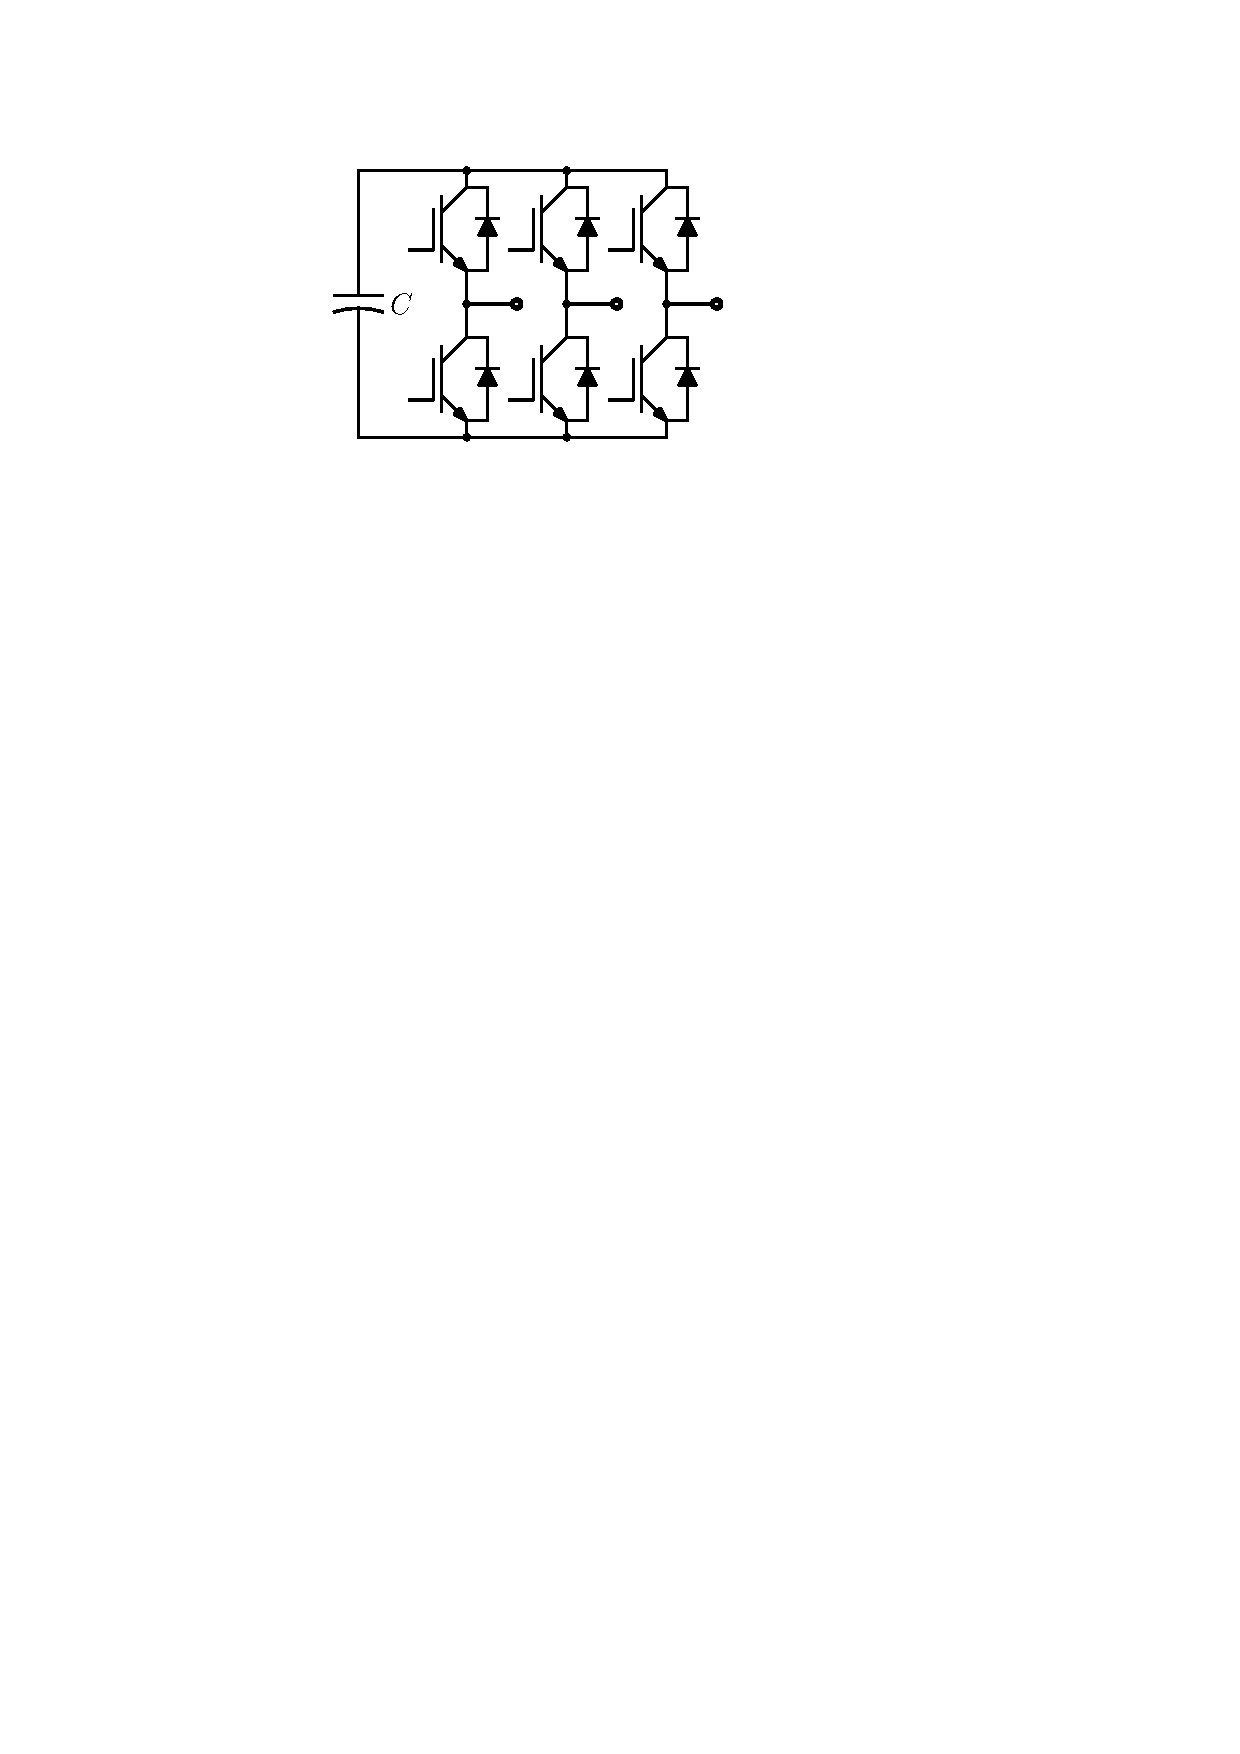
\includegraphics[width=0.8\linewidth]{./figuras/introducao/2niveis}
%
%
%\column{0.5\linewidth}
%
%\begin{itemize}
%	\item Baseados em IGBT\\[15pt]
%	\item Alta frequência de comutação\\[15pt]
%	\item Totalmente controlável\\[15pt]
%	\item Comum na industria\\[15pt]
%	\item {\color{red}Filtros (dependendo da aplicação)}\\[15pt]
%	\item {\color{red}Limitações em alta tensão}
%\end{itemize}
%
%
%
%
%\end{columns}
%
%
%
%
%
%\end{frame}





%%%%%%%%%%%%%%%%%%%%%%%%%%%%%%%%%%%%%%%%%%%%%%%%%%%%%%%
%%%%%%%%%%%%%%%%%%%%%%%%%%%%%%%%%%%%%%%%%%%%%%%%%%%%%%%
%%%%%%%%%%%%%%%%%%%%%%%%%%%%%%%%%%%%%%%%%%%%%%%%%%%%%%%
\begin{frame}{Conversores Fonte de Tensão: Dois Níveis}


\begin{columns}

\column{0.5\linewidth}
\centering

Baixa Tensão\\[20pt]

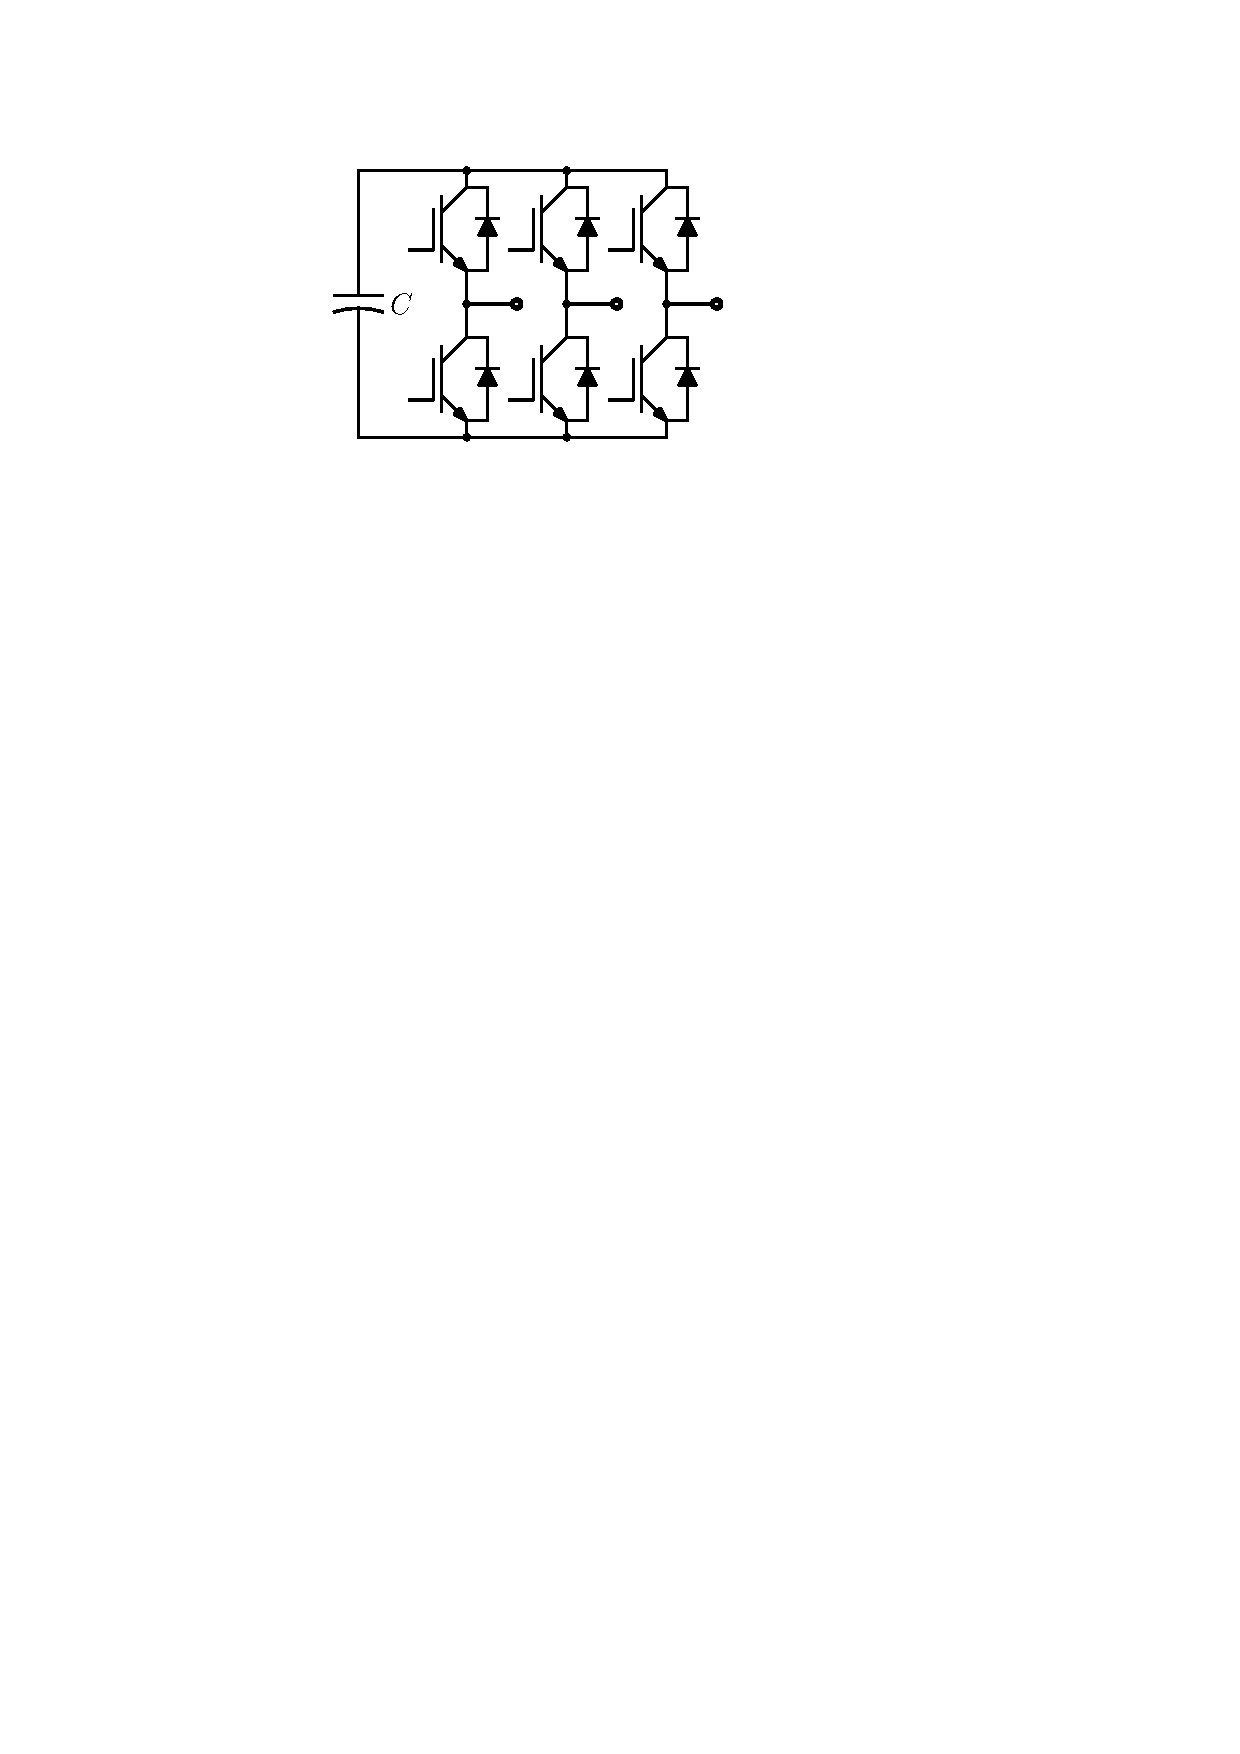
\includegraphics[width=0.6\linewidth]{./figuras/introducao/2niveis}


\column{0.5\linewidth}
\centering


Média e Alta Tensão\\[20pt]

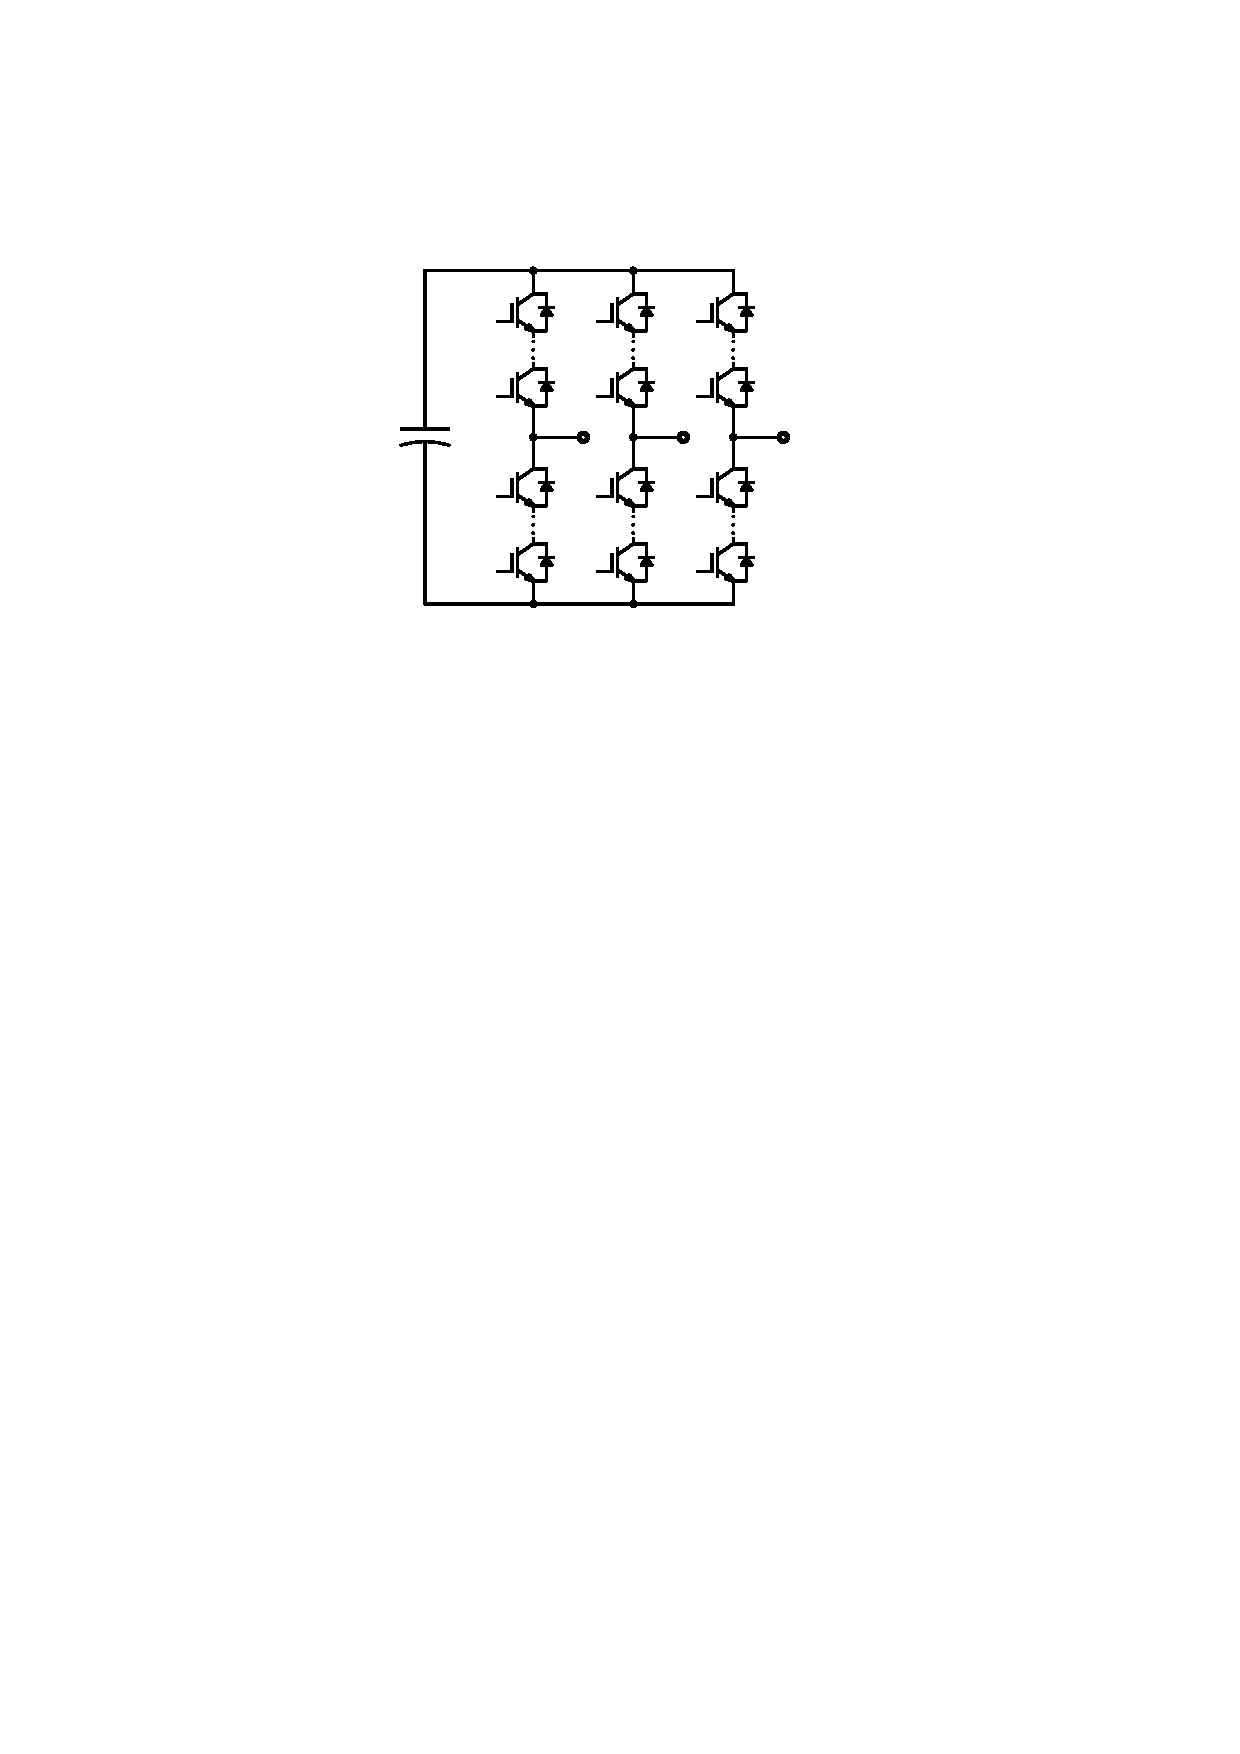
\includegraphics[width=0.55\linewidth]{./figuras/introducao/2niveis_alta}



\end{columns}





\end{frame}



%%%%%%%%%%%%%%%%%%%%%%%%%%%%%%%%%%%%%%%%%%%%%%%%%%%%%%%
%%%%%%%%%%%%%%%%%%%%%%%%%%%%%%%%%%%%%%%%%%%%%%%%%%%%%%%
%%%%%%%%%%%%%%%%%%%%%%%%%%%%%%%%%%%%%%%%%%%%%%%%%%%%%%%
\begin{frame}{Conversor Multinível Modular (MMC)}



\begin{columns}

\column{0.5\textwidth}



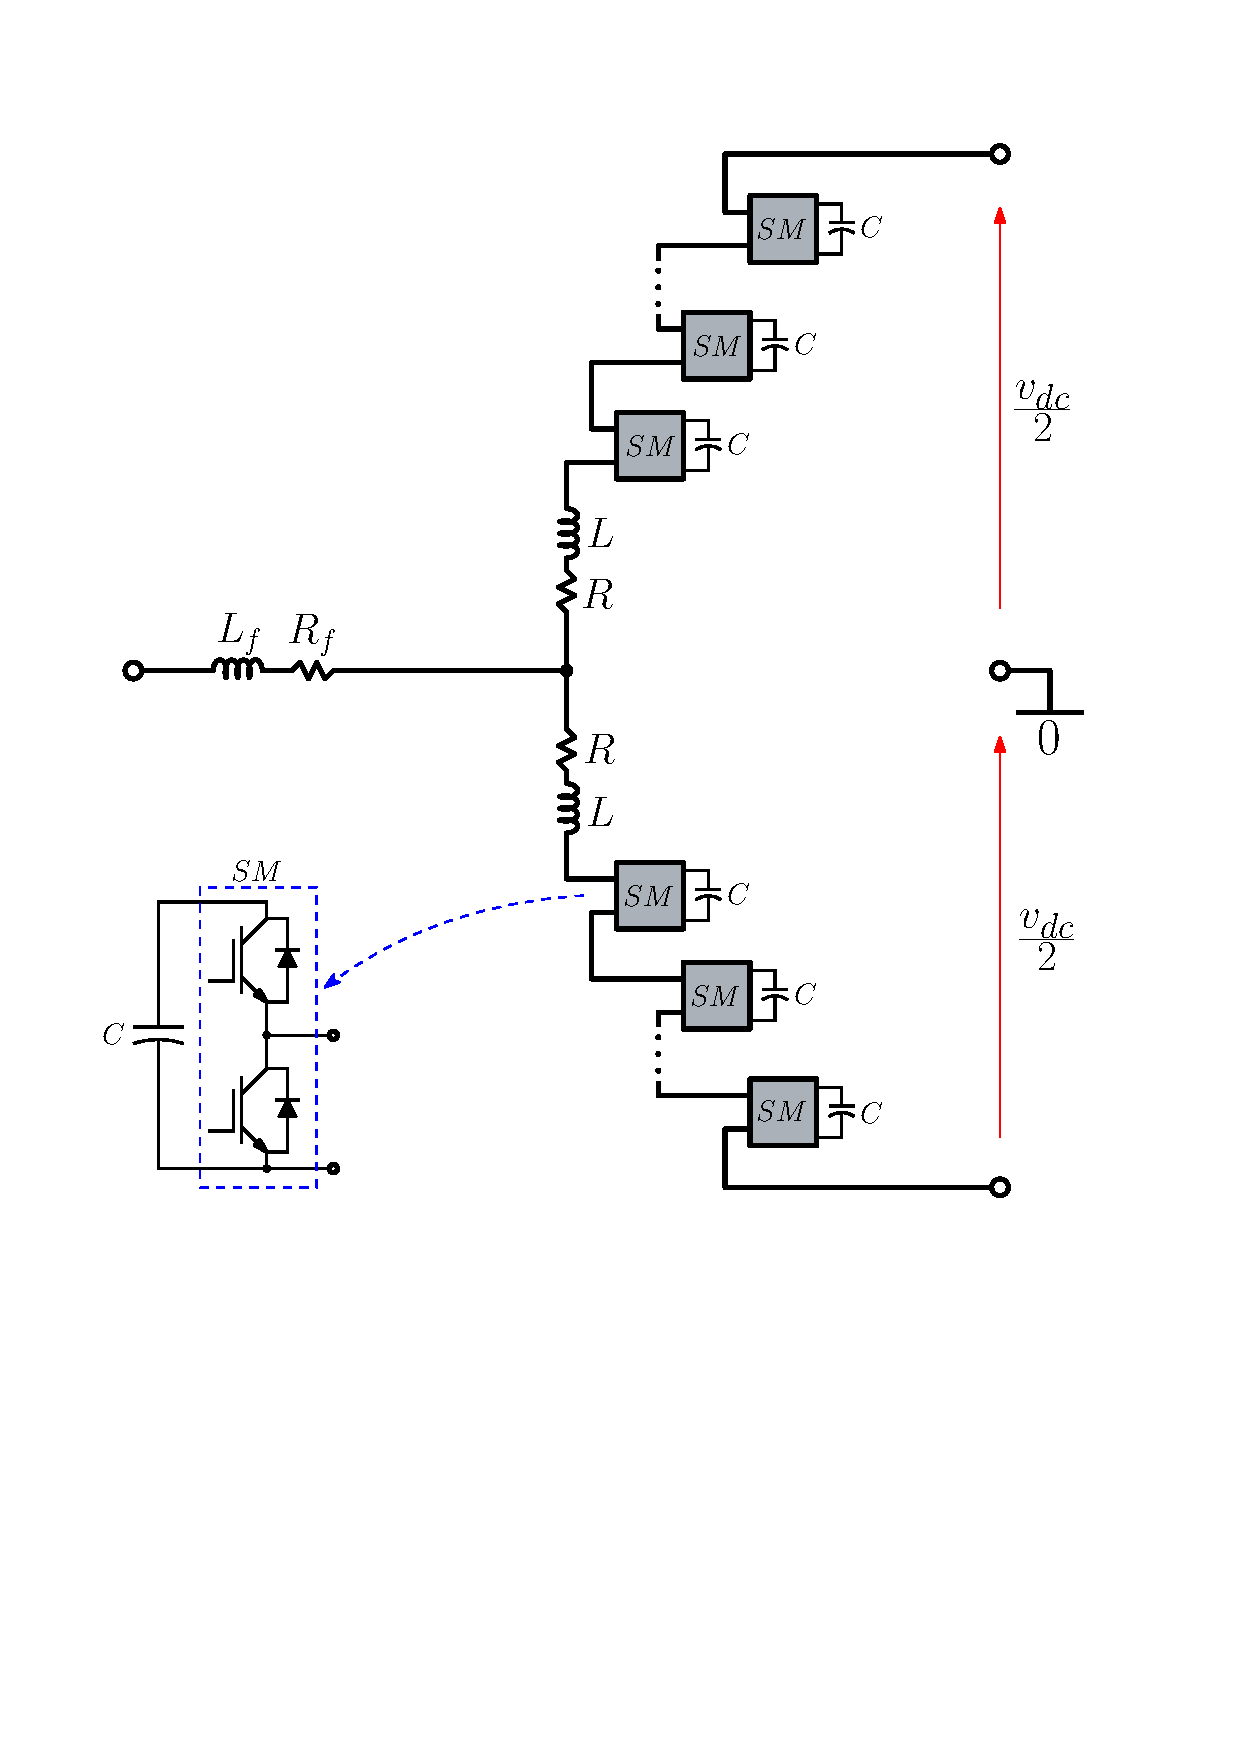
\includegraphics[width=0.9\linewidth]{./figuras/introducao/MMC_blk_limpo}







\column{0.5\textwidth}

%Aplicações

\definecolor{heavy-gray}{rgb}{0.31,0.31,0.31}




\begin{itemize}
	\item Associação de vários submódulos \\[25pt]
	\item Aplicações em alta tensão \\[25pt]
	\item Facilmente escalonável \\[25pt]
	\item {\color{blue}HVDC} \\[25pt]
	\item {\color{blue}FACTs}
\end{itemize}



\end{columns}



\end{frame}









%%%%%%%%%%%%%%%%%%%%%%%%%%%%%%%%%%%%%%%%%%%%%%%%%%%%%%%
%%%%%%%%%%%%%%%%%%%%%%%%%%%%%%%%%%%%%%%%%%%%%%%%%%%%%%%
%%%%%%%%%%%%%%%%%%%%%%%%%%%%%%%%%%%%%%%%%%%%%%%%%%%%%%%
\begin{frame}{Atualidade: Conexão de Usinas Eólicas {\it Offshore}}

\centering

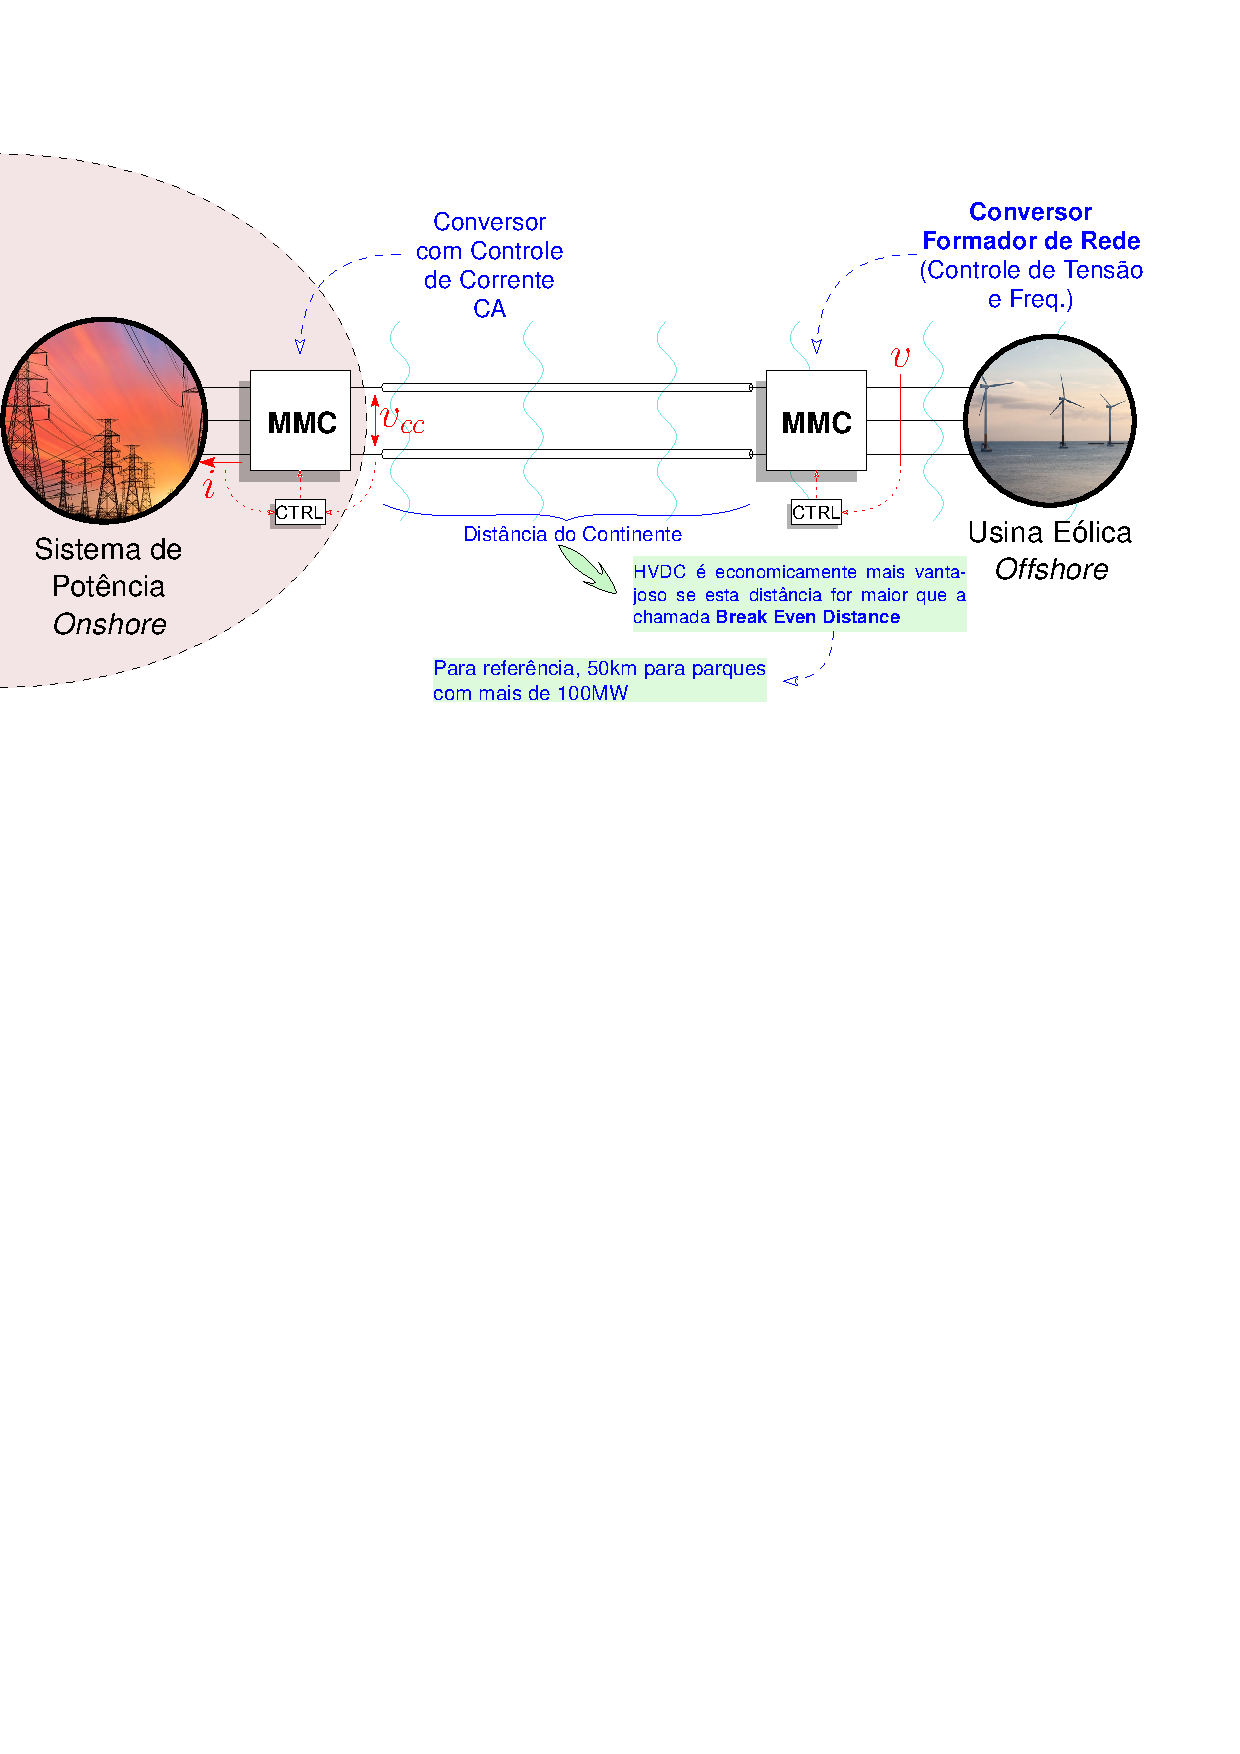
\includegraphics[width=\linewidth]{./figuras/introducao/MMC-HVDC-2}


\end{frame}











%%%%%%%%%%%%%%%%%%%%%%%%%%%%%%%%%%%%%%%%%%%%%%%%%%%%%%%
%%%%%%%%%%%%%%%%%%%%%%%%%%%%%%%%%%%%%%%%%%%%%%%%%%%%%%%
%%%%%%%%%%%%%%%%%%%%%%%%%%%%%%%%%%%%%%%%%%%%%%%%%%%%%%%
\begin{frame}{Foco do Trabalho}



\begin{itemize}
	\item Obter modelos matemáticos analíticos no domínio da frequência considerando diferentes modos de controle: 
	
	\begin{itemize}
		\item Controle por corrente CA
		\item Controle por tensão CA (formador de rede)
		\item Controle em referencial natural
		\item Controle em referencial síncrono
	\end{itemize}

	\item Realizar análises:
	
	\begin{itemize}
		\item Influência dos controladores
		\item Derivações de impedâncias/admitâncias virtuais para melhorar a performance do MMC
	\end{itemize}
	
	\item Apresentar aplicação:
	
	\begin{itemize}
		\item Análise de estabilidade de sistemas baseados em MMC
	\end{itemize}
	
	
\end{itemize}










%Modelos em referencial natural e em referencial síncrono para o MMC formador de rede com malha dupla (corrente e tensão).


%
%\begin{itemize}
%	\item Será focada nos modelos ;
%	
%	\item Considerar um banco capacitivo $C_f$ (...)
%	
%	\item Obter o modelo para a malha de corrente
%	
%	\item Obter um modelo para malha de tensão sem considerar $C_f$
%	
%	\item Incluir $C_f$ no modelo.
%\end{itemize}


\end{frame}






\cmfnewsection{Visão Geral do PSCAD e do Curso}{./logos/fundo_tese}{0.15}






%%%%%%%%%%%%%%%%%%%%%%%%%%%%%%%%%%%%%%%%%%%%%%%%
%%%%%%%%%%%%%%%%%%%%%%%%%%%%%%%%%%%%%%%%%%%%%%%%
%%%%%%%%%%%%%%%%%%%%%%%%%%%%%%%%%%%%%%%%%%%%%%%%
%%%%%%%%%%%%%%%%%%%%%%%%%%%%%%%%%%%%%%%%%%%%%%%%
\begin{frame}{Objetivo}
\centering

\begin{itemize}
\item Aprender a montar simulações de sistemas elétricos no PSCAD 
\vspace*{1cm}
\item Aprender a extrair resultados
\vspace*{1cm}
\item Possivelmente, aprender o funcionamento de alguns circuitos básicos.
\vspace*{1cm}
\end{itemize}

\end{frame}






%%%%%%%%%%%%%%%%%%%%%%%%%%%%%%%%%%%%%%%%%%%%%%%%
%%%%%%%%%%%%%%%%%%%%%%%%%%%%%%%%%%%%%%%%%%%%%%%%
%%%%%%%%%%%%%%%%%%%%%%%%%%%%%%%%%%%%%%%%%%%%%%%%
%%%%%%%%%%%%%%%%%%%%%%%%%%%%%%%%%%%%%%%%%%%%%%%%
\begin{frame}{O que é o PSCAD}
\centering

\begin{itemize}
\item O PSCAD ({\it Power Systems Computer Aided Design}) é uma interface gráfica para simulação no EMTDC

\vspace*{2cm}

\item o EMTDC é um programa utilizado para simulação de transitórios eletromagnéticos.
\end{itemize}

\end{frame}





%%%%%%%%%%%%%%%%%%%%%%%%%%%%%%%%%%%%%%%%%%%%%%%%
%%%%%%%%%%%%%%%%%%%%%%%%%%%%%%%%%%%%%%%%%%%%%%%%
%%%%%%%%%%%%%%%%%%%%%%%%%%%%%%%%%%%%%%%%%%%%%%%%
%%%%%%%%%%%%%%%%%%%%%%%%%%%%%%%%%%%%%%%%%%%%%%%%
\begin{frame}{Para que serve o PSCAD}
\centering

\begin{itemize}
\item Simulação de sistemas de potência: transitórios eletromagnéticos

\begin{itemize}
\item Redes de distribuição e transmissão
\item Máquinas Elétricas
\item Sistemas de controle de fontes de energia
\end{itemize}

\vspace*{1cm}

\item Simulação de sistemas envolvendo eletrônica de potência.

\begin{itemize}
\item Grid-connected/Grid-Forming Converters
\item HVDCs ({\it High Voltage Direct Current})
\item FACTS ({\it flexible alternating current transmission system})
\item Sistemas de controle
\end{itemize}

\end{itemize}

\end{frame}





%%%%%%%%%%%%%%%%%%%%%%%%%%%%%%%%%%%%%%%%%%%%%%%%
%%%%%%%%%%%%%%%%%%%%%%%%%%%%%%%%%%%%%%%%%%%%%%%%
%%%%%%%%%%%%%%%%%%%%%%%%%%%%%%%%%%%%%%%%%%%%%%%%
%%%%%%%%%%%%%%%%%%%%%%%%%%%%%%%%%%%%%%%%%%%%%%%%
\begin{frame}{Ideia Geral do PSCAD}
\centering


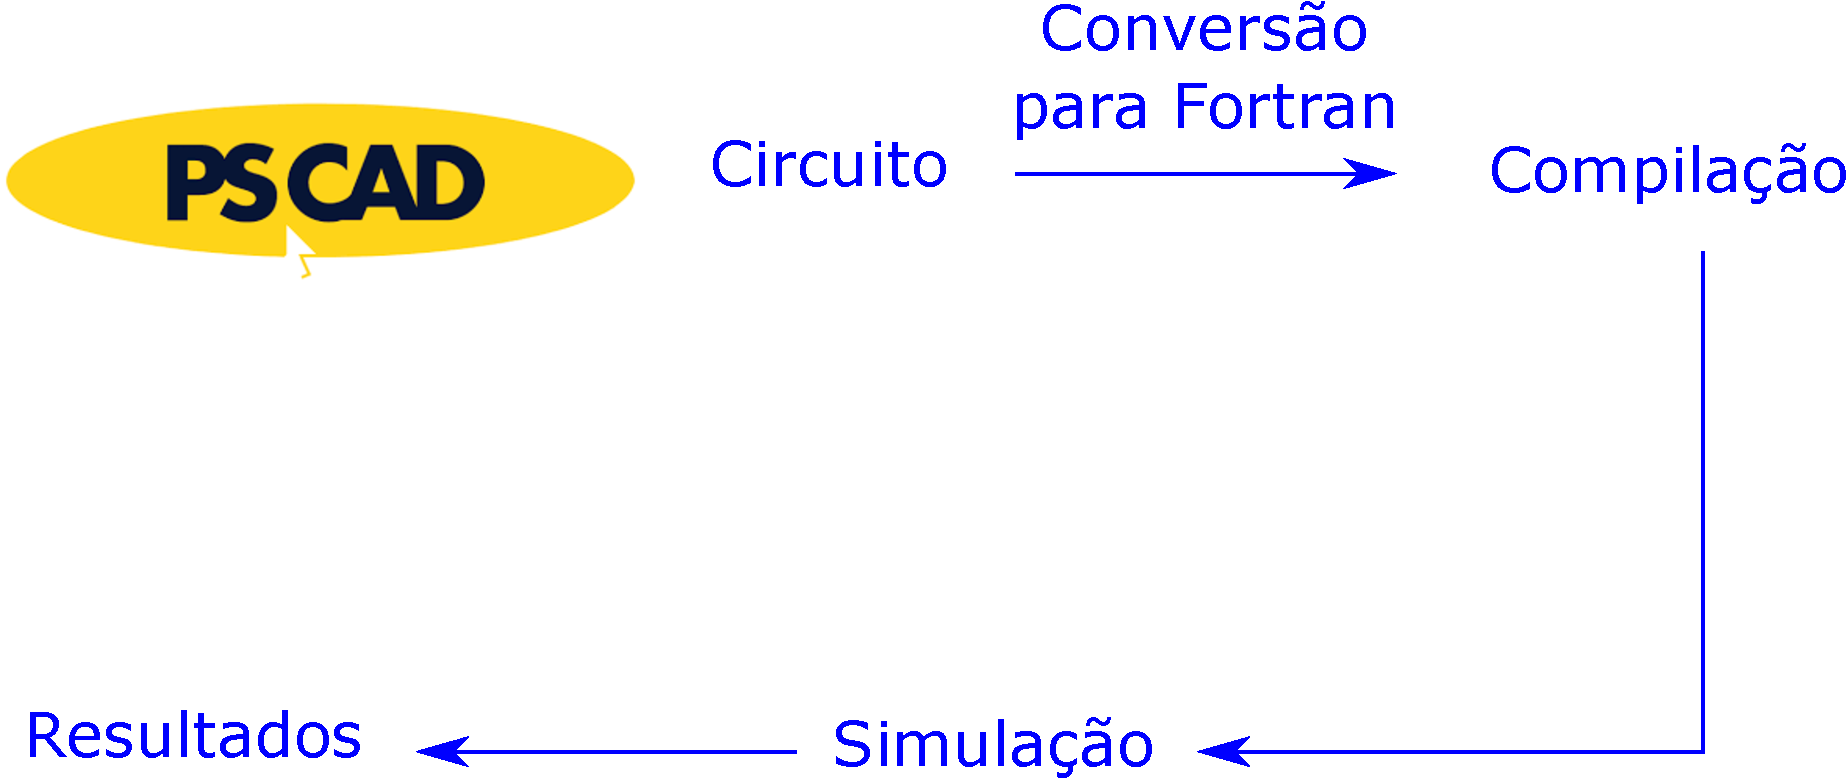
\includegraphics[width=0.95\linewidth]{./figuras/geral/fluxo}

\end{frame}

\cmfnewsection{Primeiros Passos no PSCAD}{./logos/fundo_tese}{0.15}





%%%%%%%%%%%%%%%%%%%%%%%%%%%%%%%%%%%%%%%%%%%%%%%%
%%%%%%%%%%%%%%%%%%%%%%%%%%%%%%%%%%%%%%%%%%%%%%%%
%%%%%%%%%%%%%%%%%%%%%%%%%%%%%%%%%%%%%%%%%%%%%%%%
%%%%%%%%%%%%%%%%%%%%%%%%%%%%%%%%%%%%%%%%%%%%%%%%
\begin{frame}{PSCAD: Versão Gratuita}
\centering

\begin{columns}
\column{0.3\linewidth}
apenas um teste

\column{0.7\linewidth}
\centering
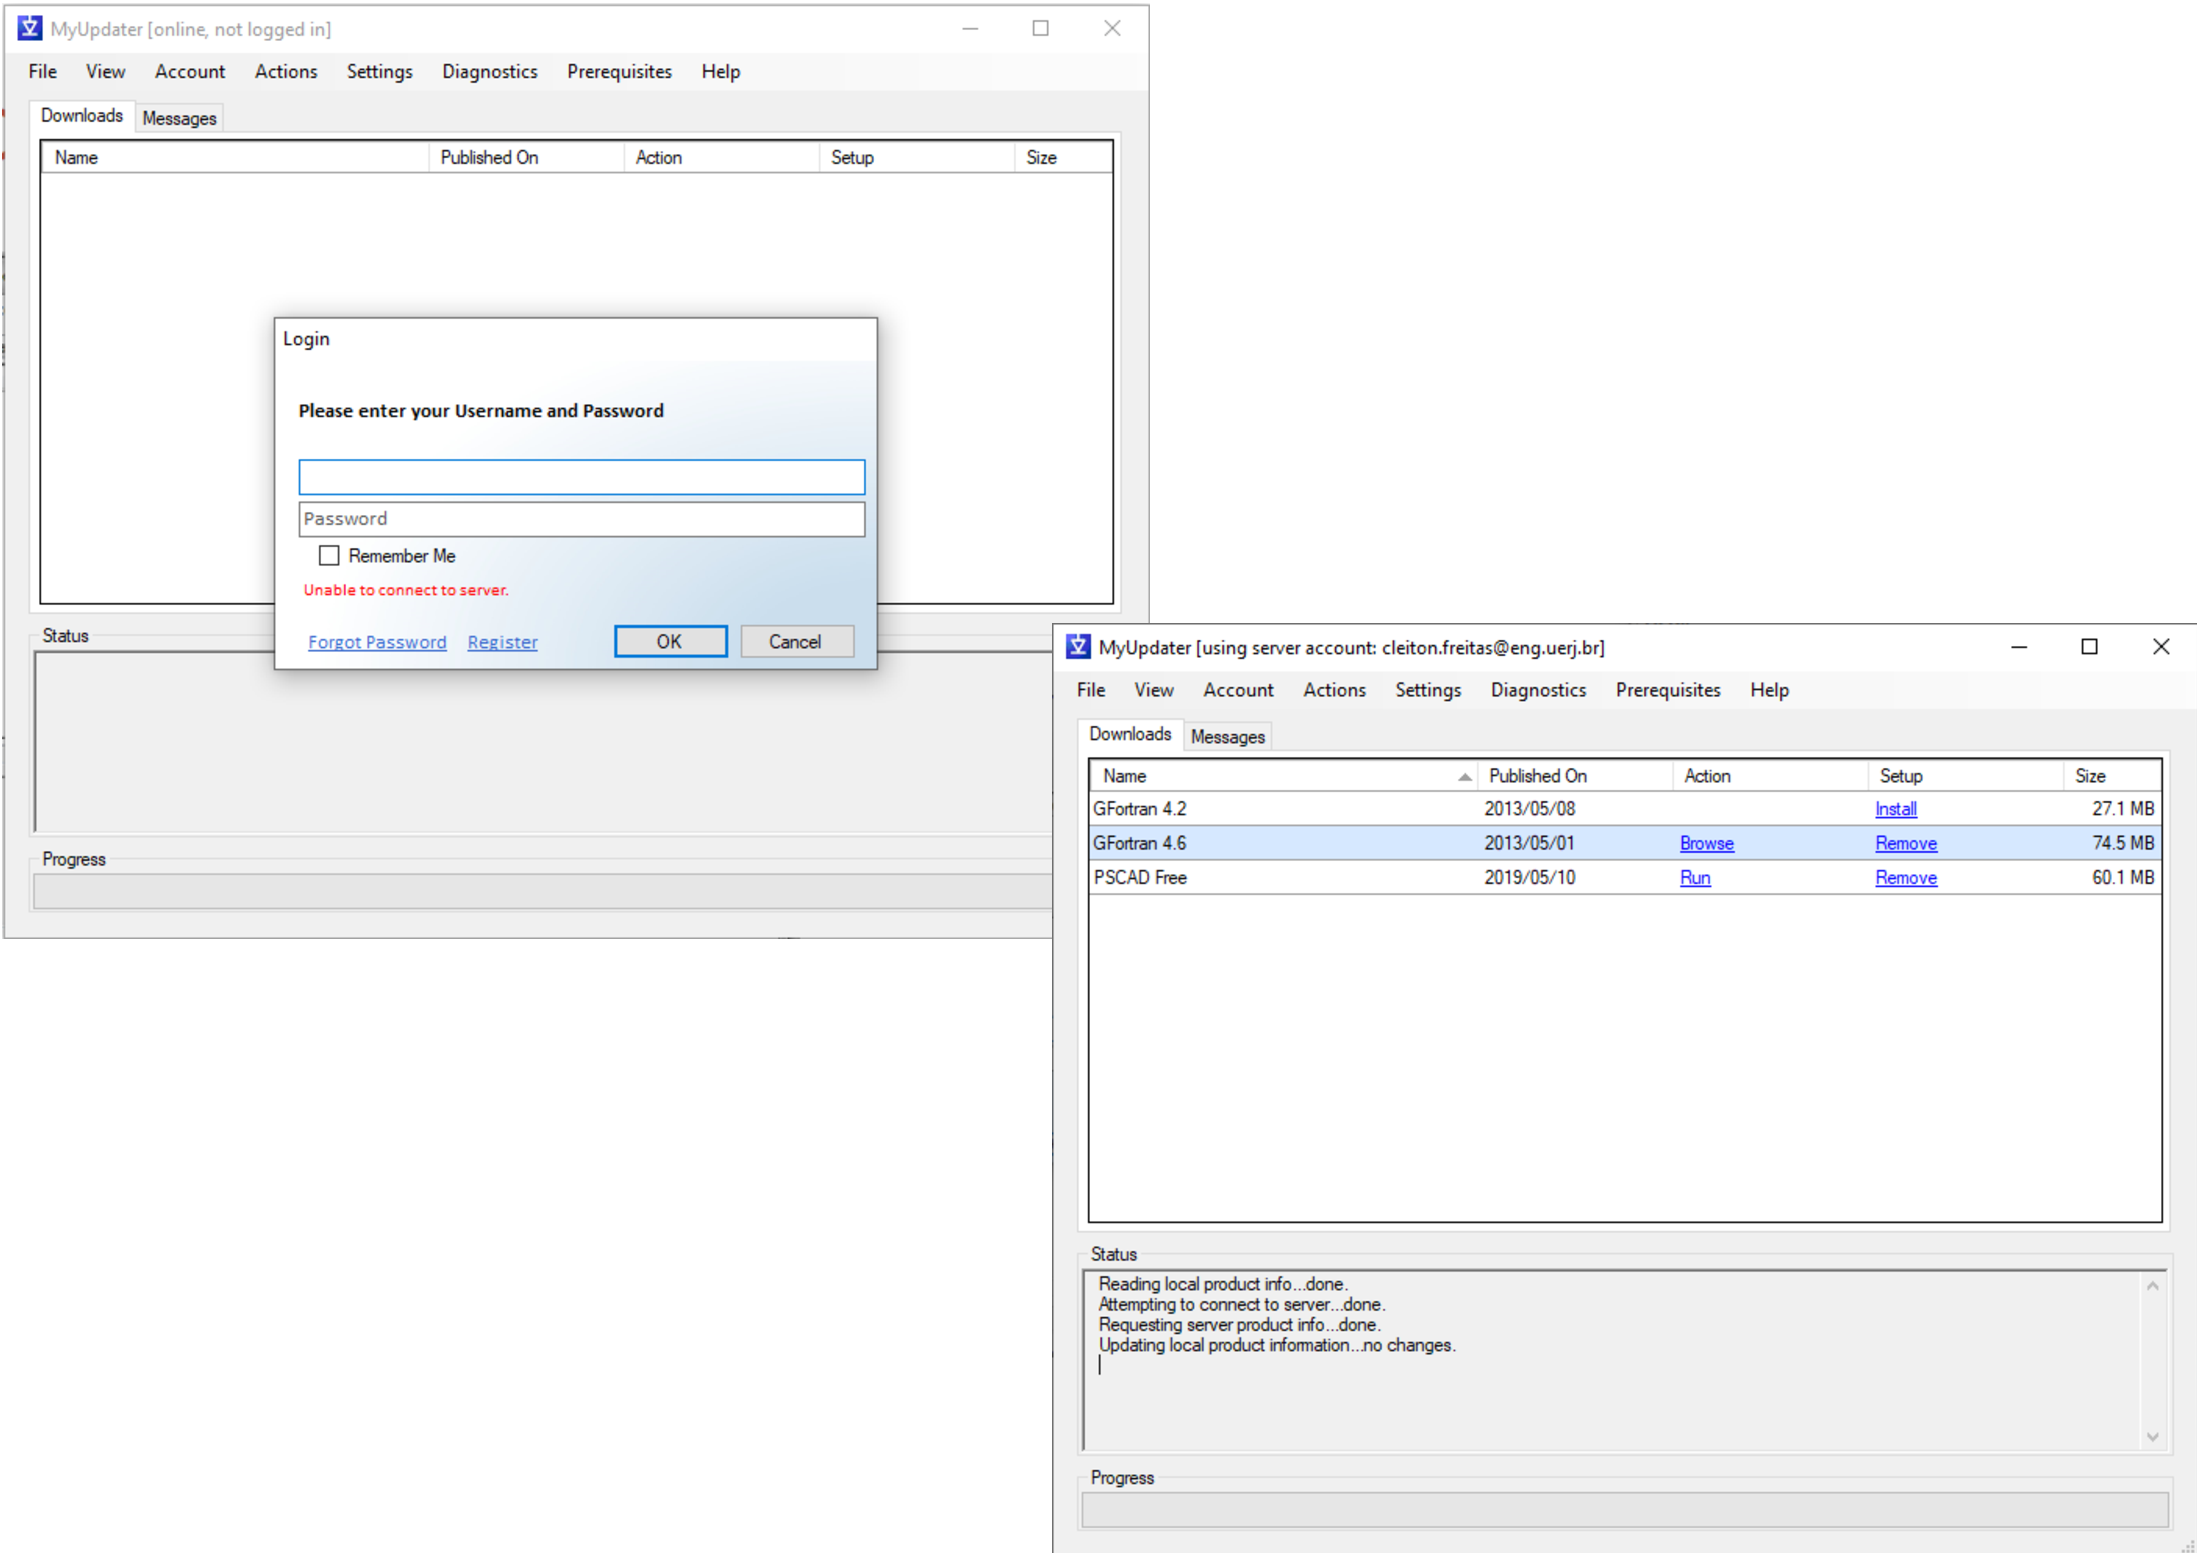
\includegraphics[width=0.8\linewidth]{./figuras/Primeiros-Passos/login}

\end{columns}

\end{frame}


%%%%%%%%%%%%%%%%%%%%%%%%%%%%%%%%%%%%%%%%%%%%%%%%
%%%%%%%%%%%%%%%%%%%%%%%%%%%%%%%%%%%%%%%%%%%%%%%%
%%%%%%%%%%%%%%%%%%%%%%%%%%%%%%%%%%%%%%%%%%%%%%%%
%%%%%%%%%%%%%%%%%%%%%%%%%%%%%%%%%%%%%%%%%%%%%%%%
\begin{frame}{PSCAD: Versão Gratuita}
\centering


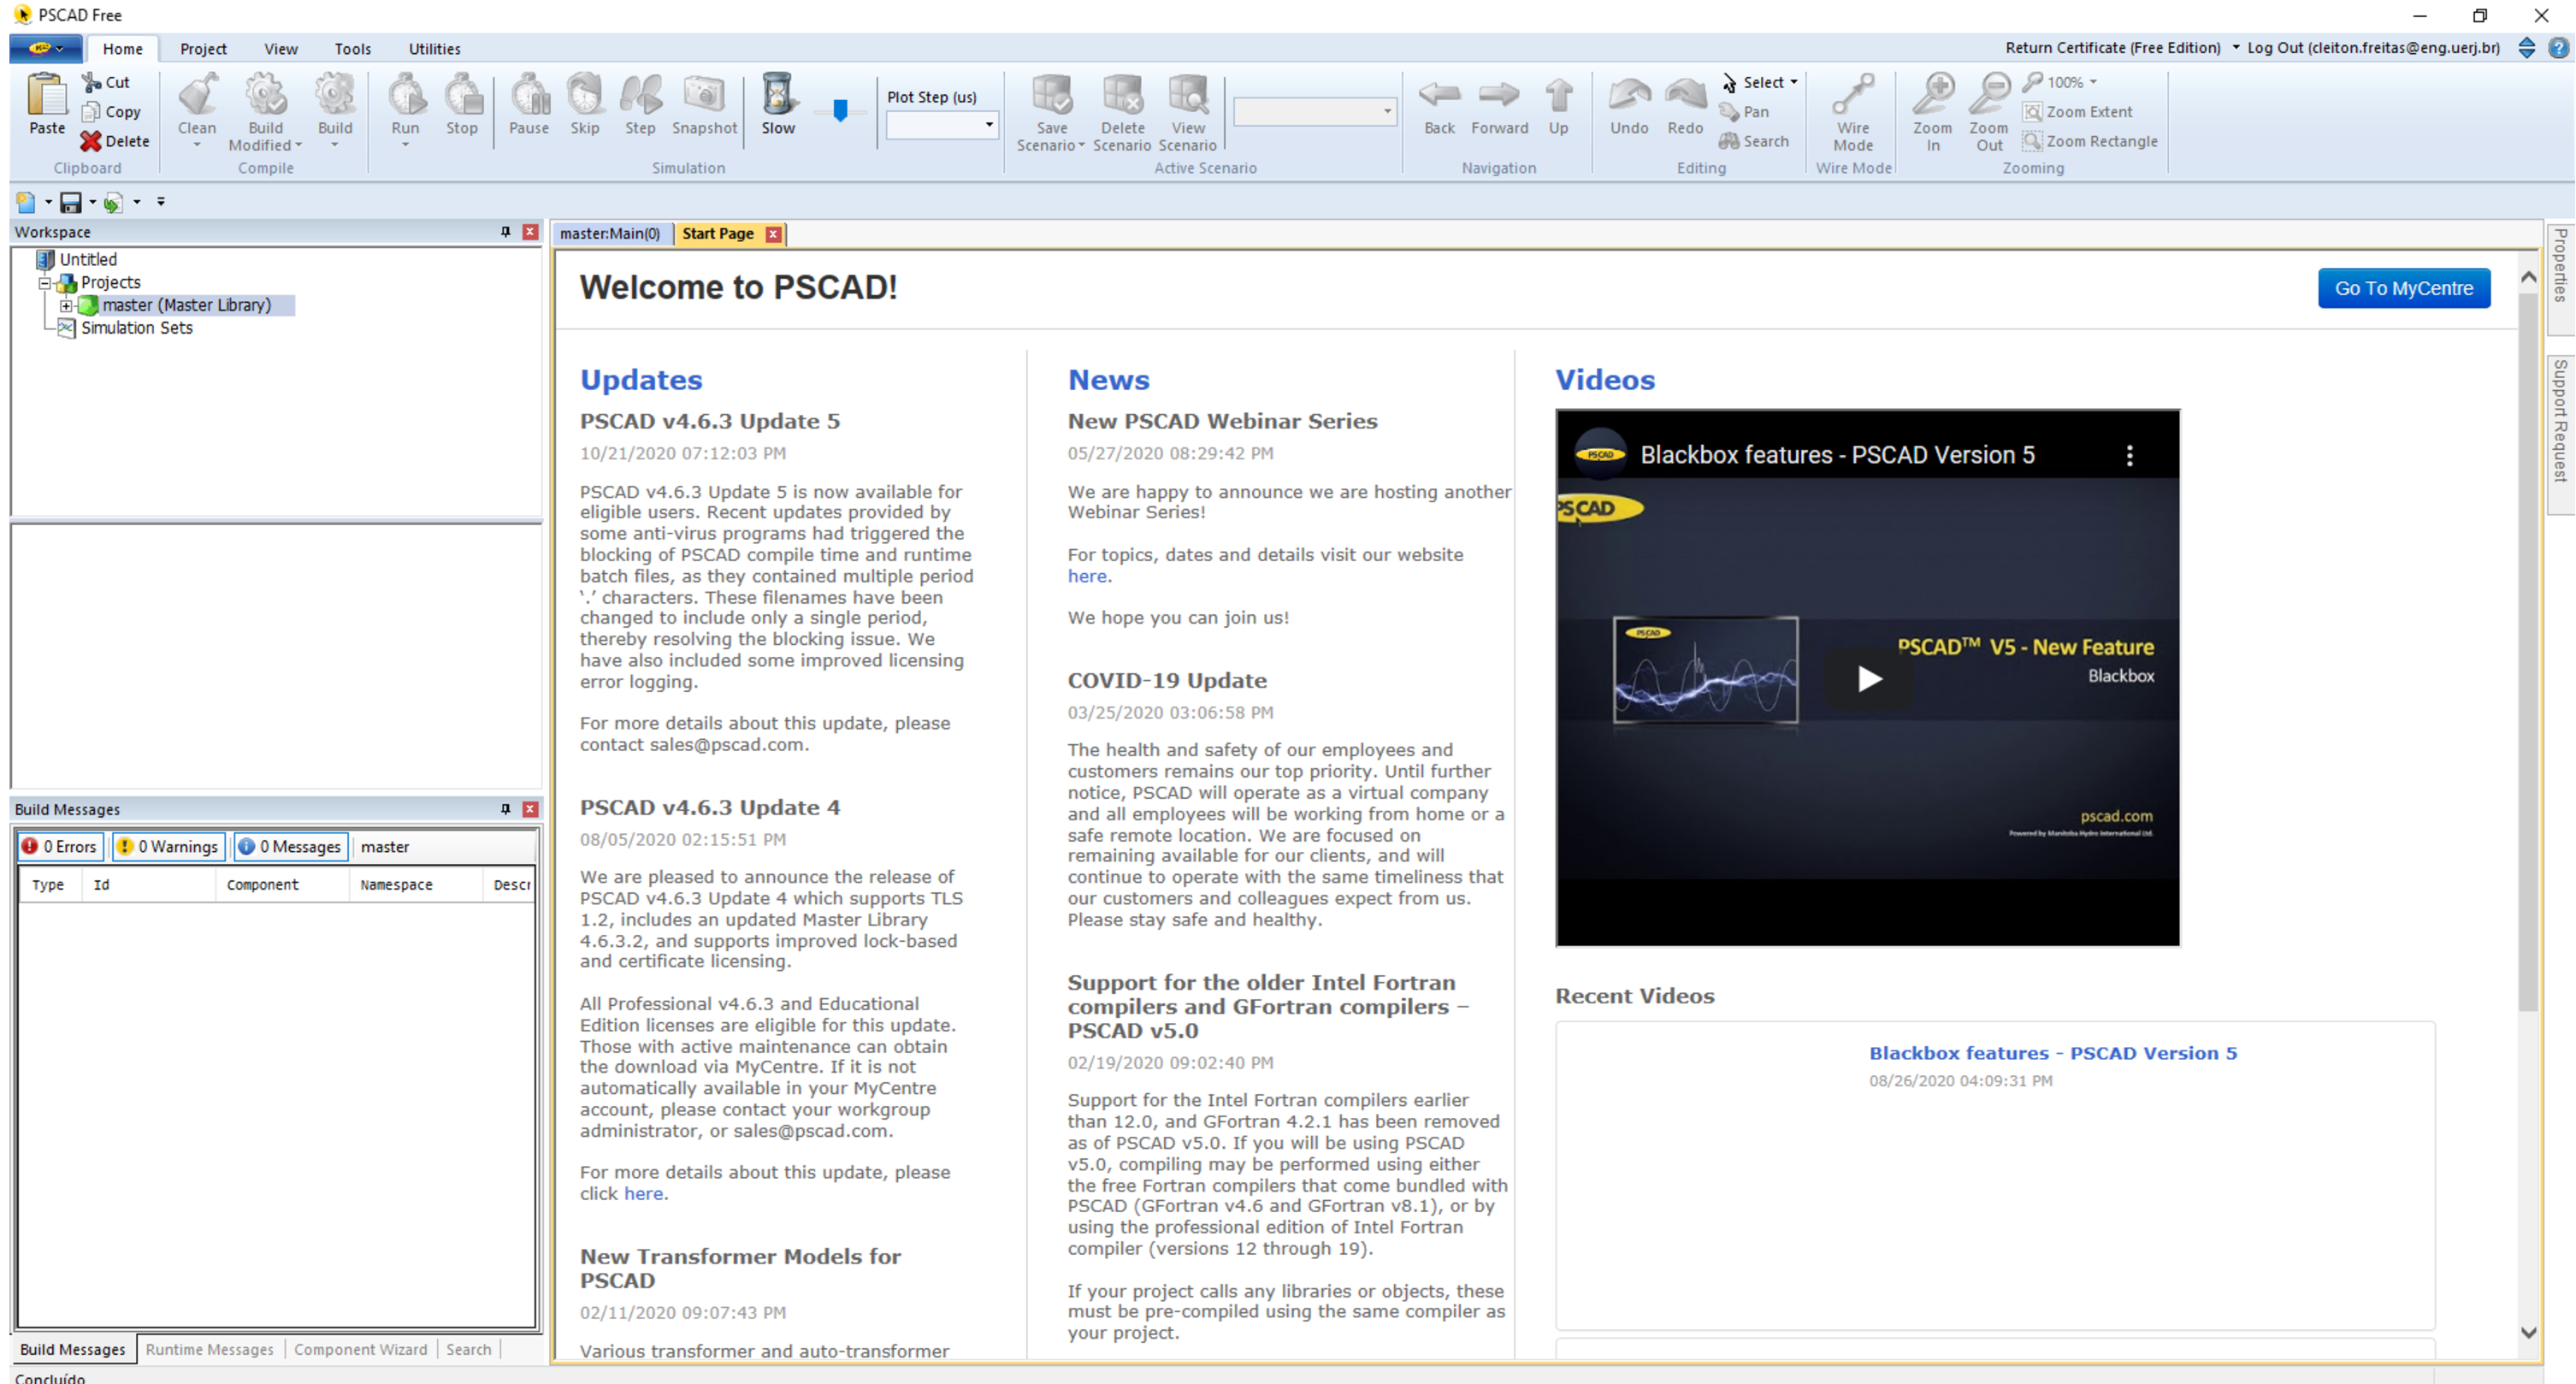
\includegraphics[width=0.85\linewidth]{./figuras/Primeiros-Passos/tela_inicial}


\end{frame}





%%%%%%%%%%%%%%%%%%%%%%%%%%%%%%%%%%%%%%%%%%%%%%%%
%%%%%%%%%%%%%%%%%%%%%%%%%%%%%%%%%%%%%%%%%%%%%%%%
%%%%%%%%%%%%%%%%%%%%%%%%%%%%%%%%%%%%%%%%%%%%%%%%
%%%%%%%%%%%%%%%%%%%%%%%%%%%%%%%%%%%%%%%%%%%%%%%%
\begin{frame}{PSCAD: Biblioteca Master}
\centering


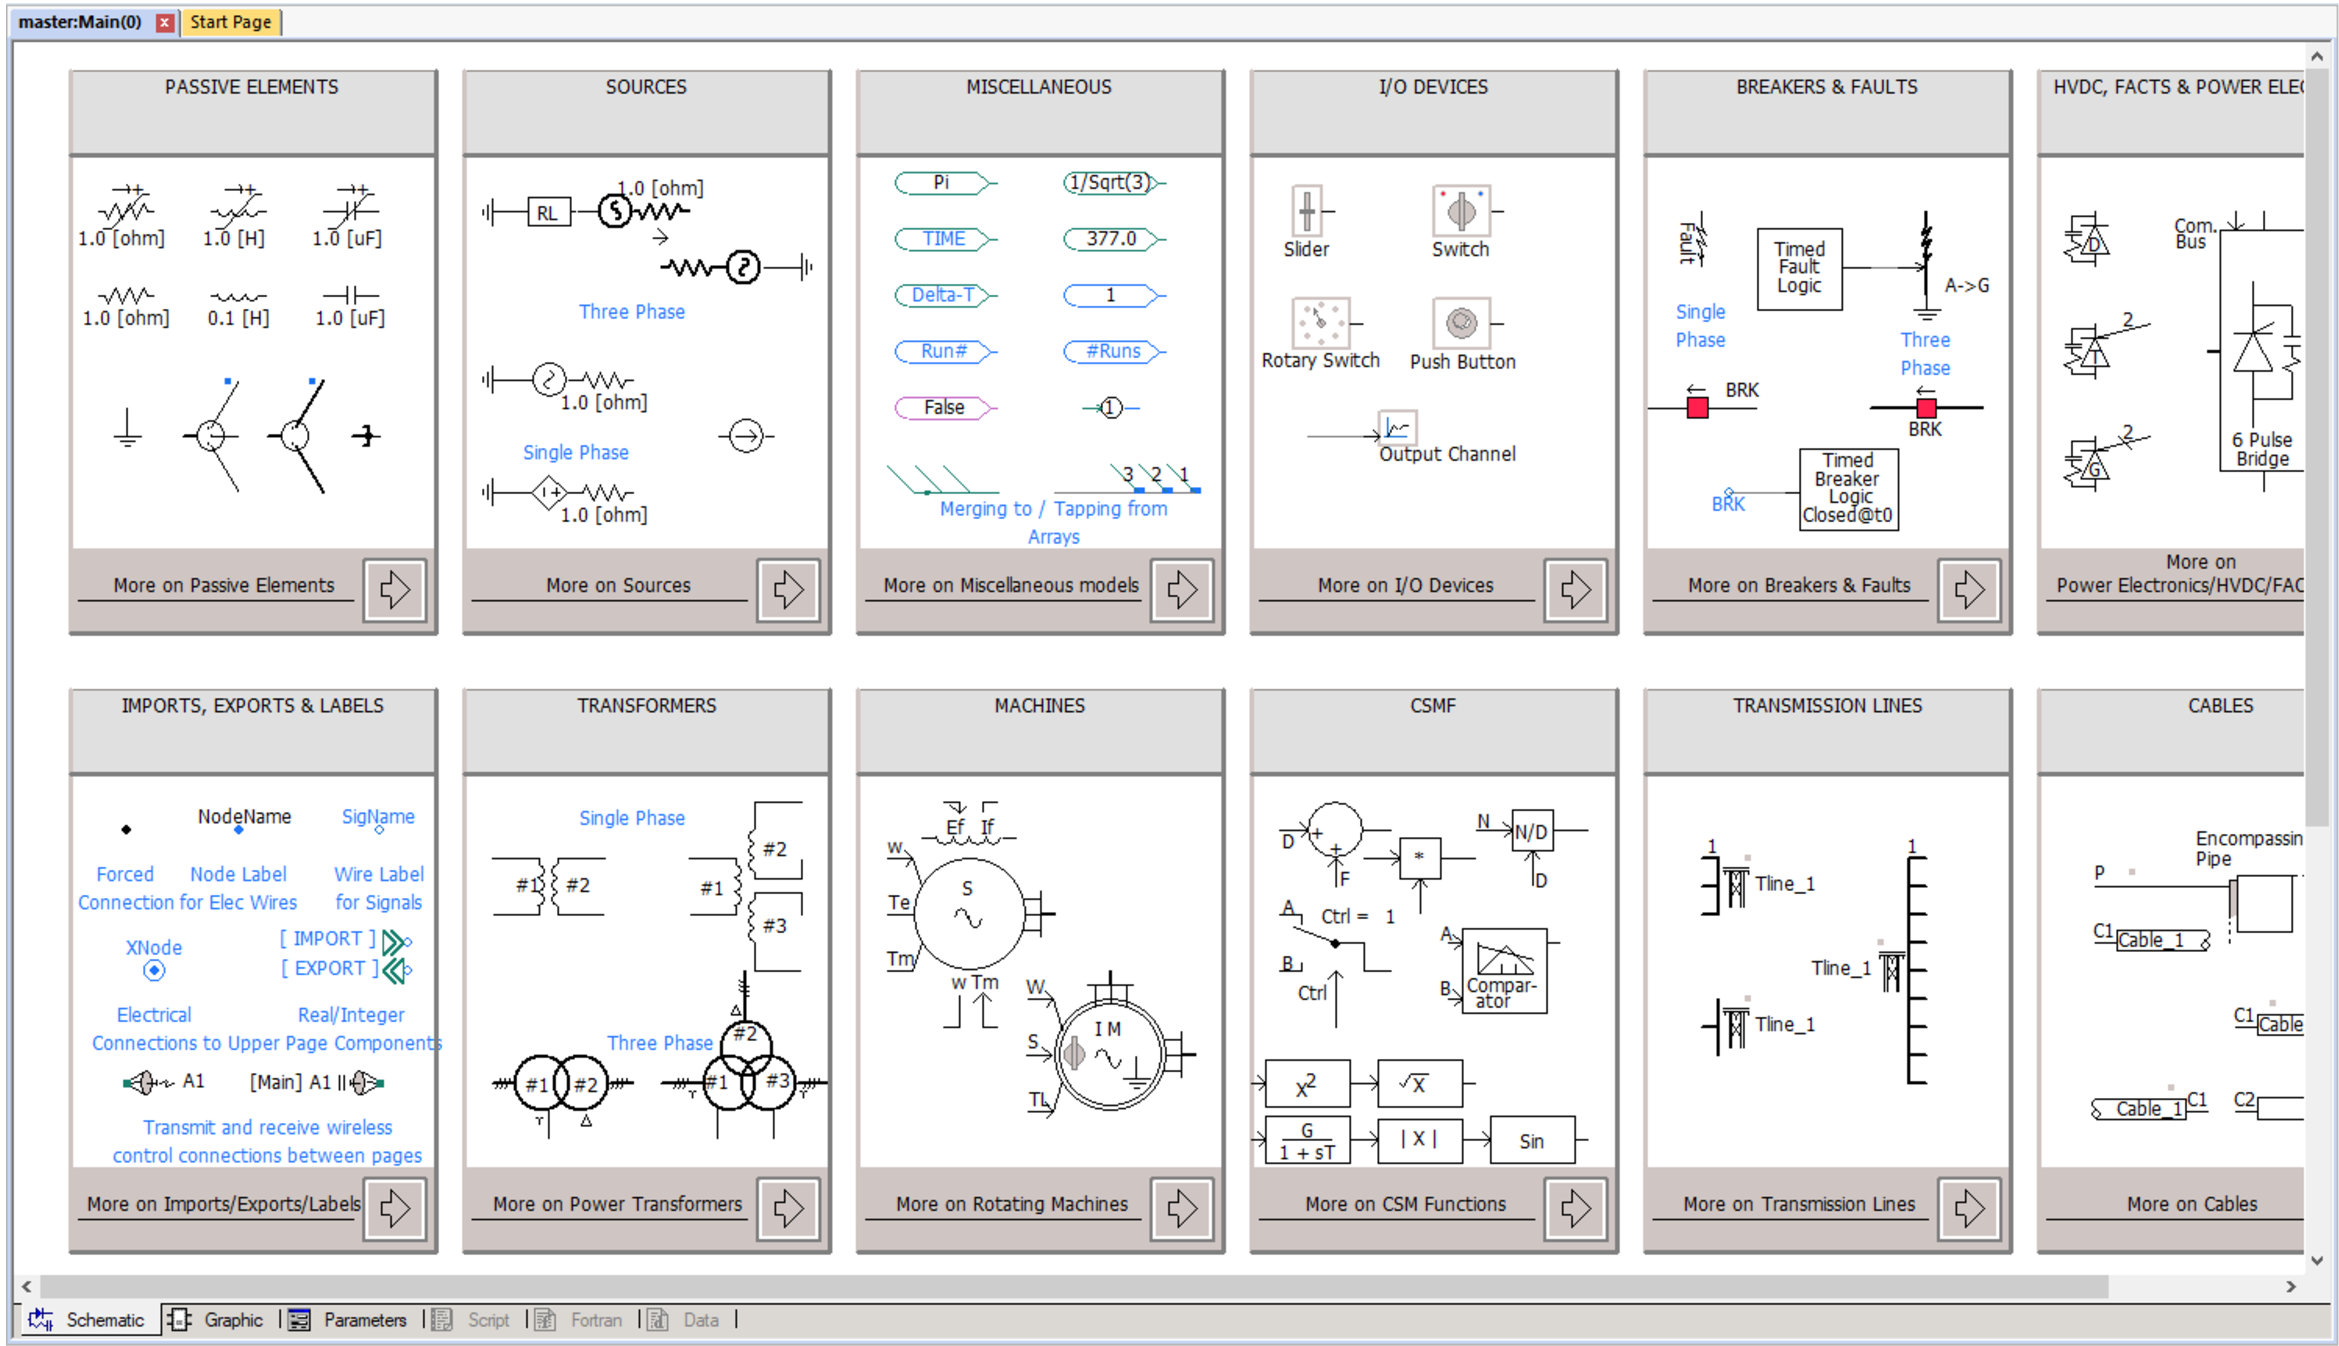
\includegraphics[width=0.85\linewidth]{./figuras/Primeiros-Passos/biblioteca_master}


\end{frame}




%%%%%%%%%%%%%%%%%%%%%%%%%%%%%%%%%%%%%%%%%%%%%%%%
%%%%%%%%%%%%%%%%%%%%%%%%%%%%%%%%%%%%%%%%%%%%%%%%
%%%%%%%%%%%%%%%%%%%%%%%%%%%%%%%%%%%%%%%%%%%%%%%%
%%%%%%%%%%%%%%%%%%%%%%%%%%%%%%%%%%%%%%%%%%%%%%%%
\begin{frame}{PSCAD: Biblioteca Master}
\centering


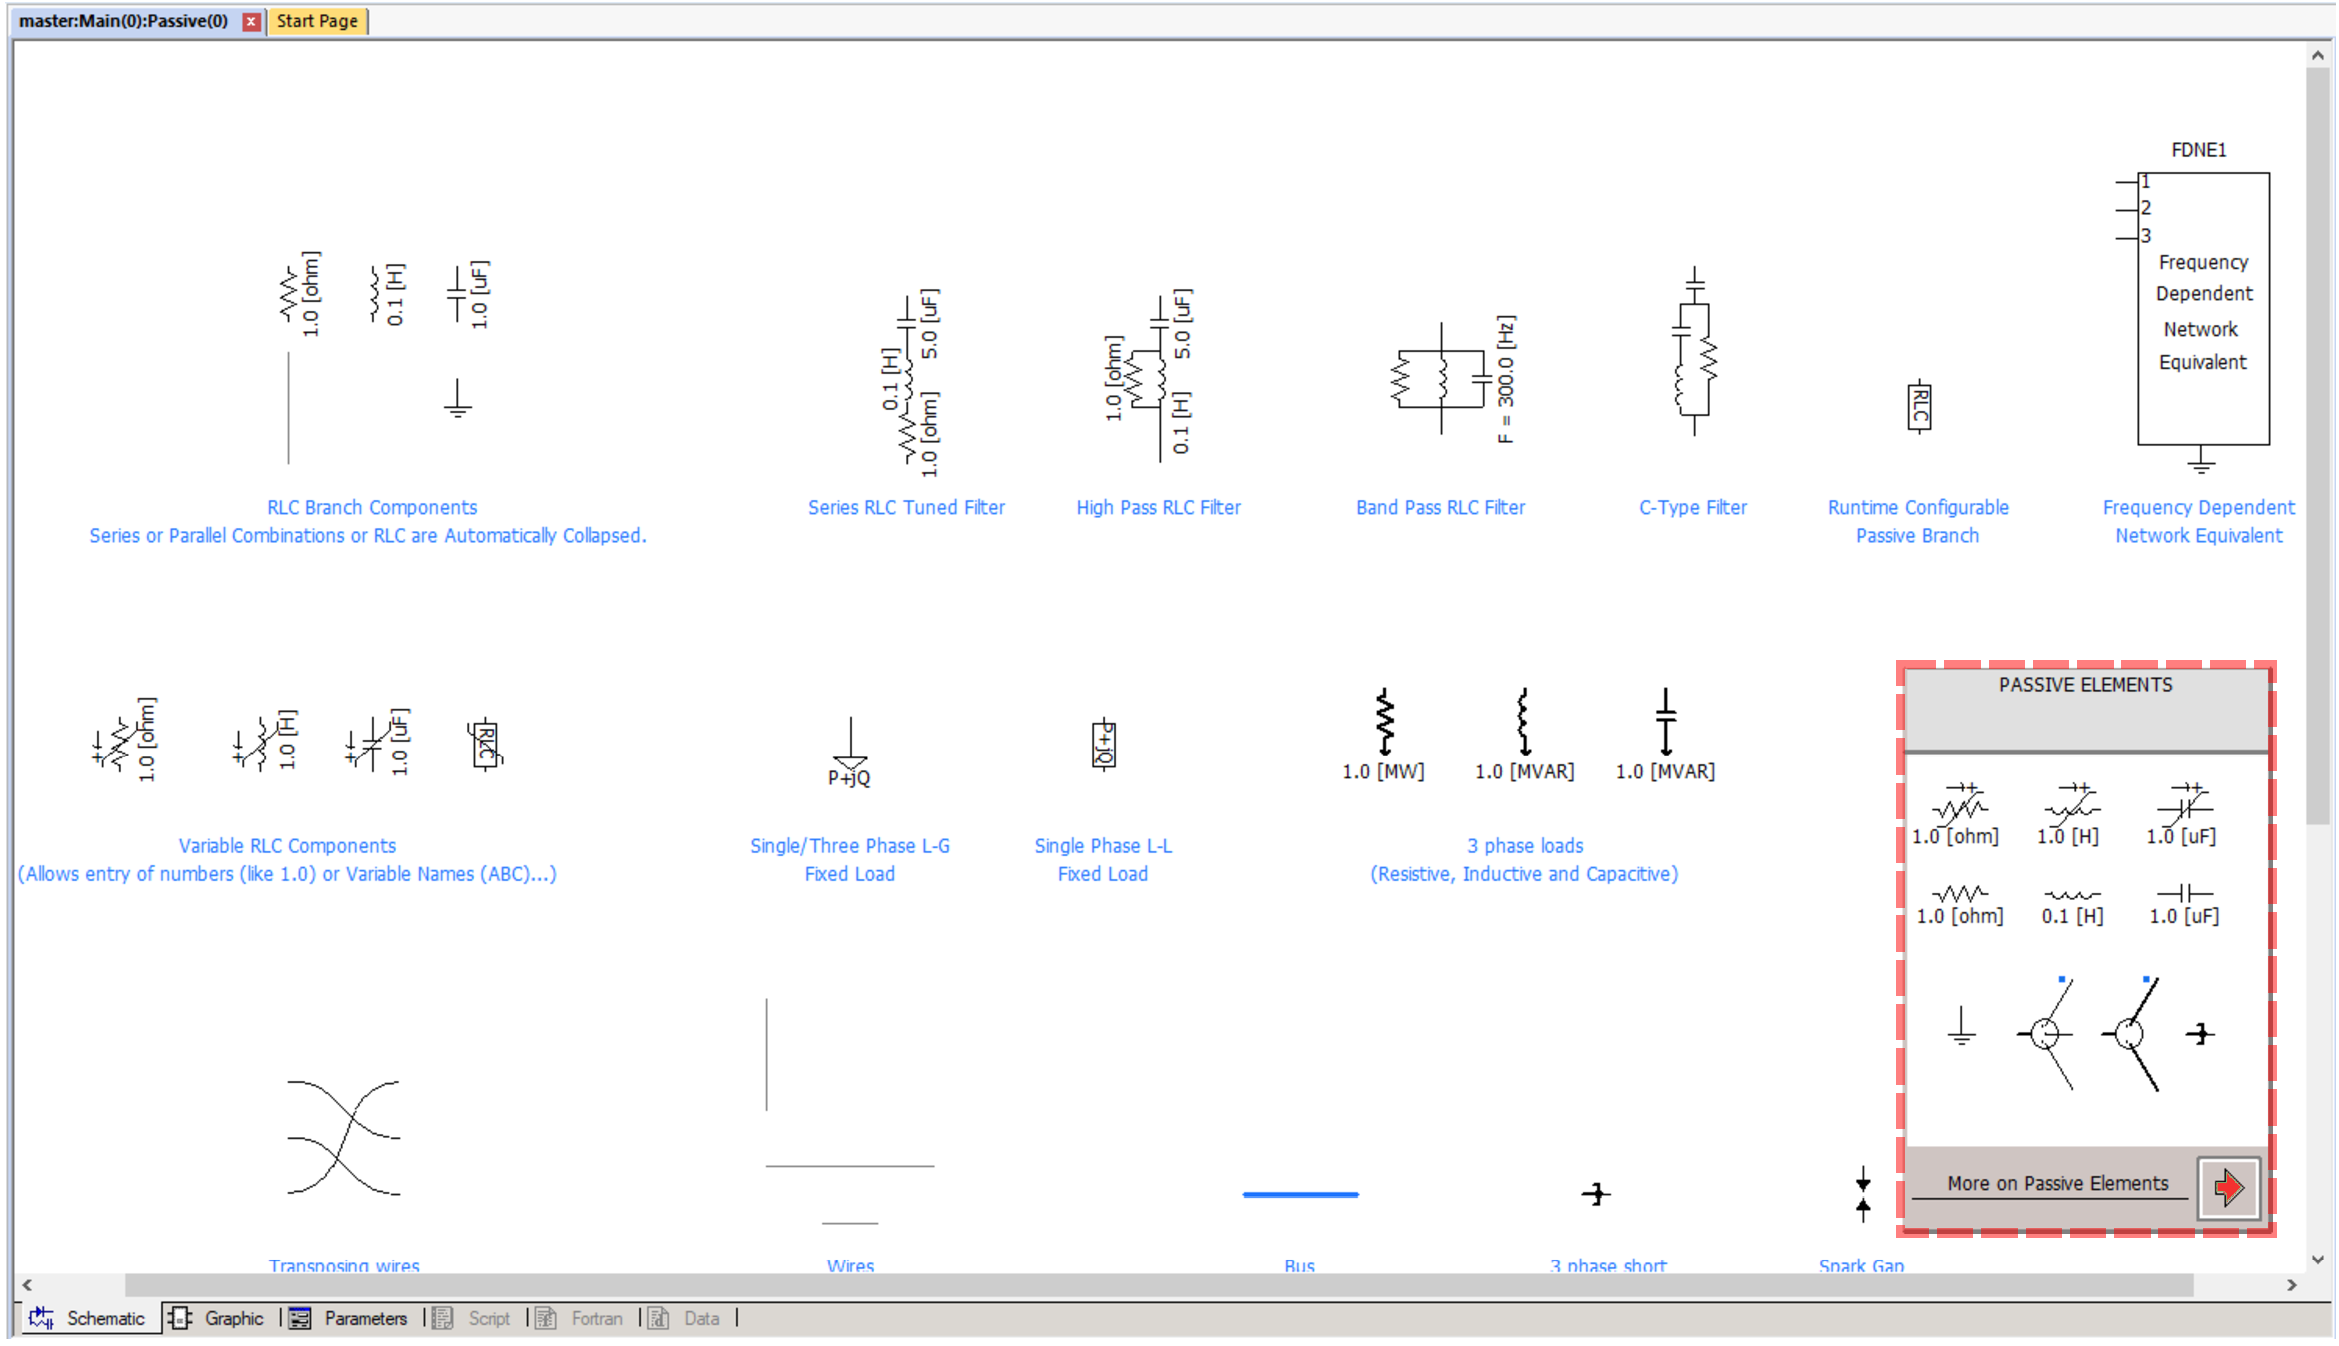
\includegraphics[width=0.85\linewidth]{./figuras/Primeiros-Passos/biblioteca_parte}


\end{frame}





%%%%%%%%%%%%%%%%%%%%%%%%%%%%%%%%%%%%%%%%%%%%%%%%
%%%%%%%%%%%%%%%%%%%%%%%%%%%%%%%%%%%%%%%%%%%%%%%%
%%%%%%%%%%%%%%%%%%%%%%%%%%%%%%%%%%%%%%%%%%%%%%%%
%%%%%%%%%%%%%%%%%%%%%%%%%%%%%%%%%%%%%%%%%%%%%%%%
\begin{frame}{PSCAD: Biblioteca Master}
\centering


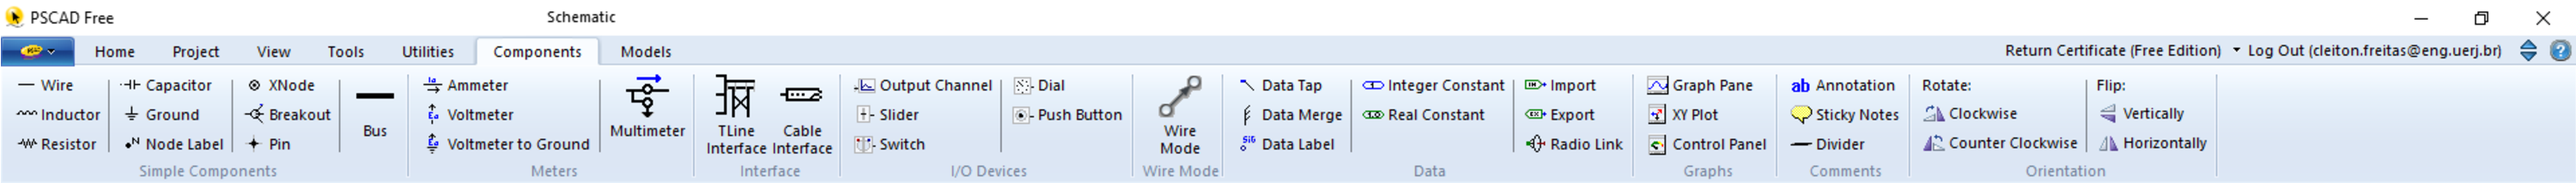
\includegraphics[width=0.85\linewidth]{./figuras/Primeiros-Passos/biblioteca_barra_components}
\vspace*{1cm}

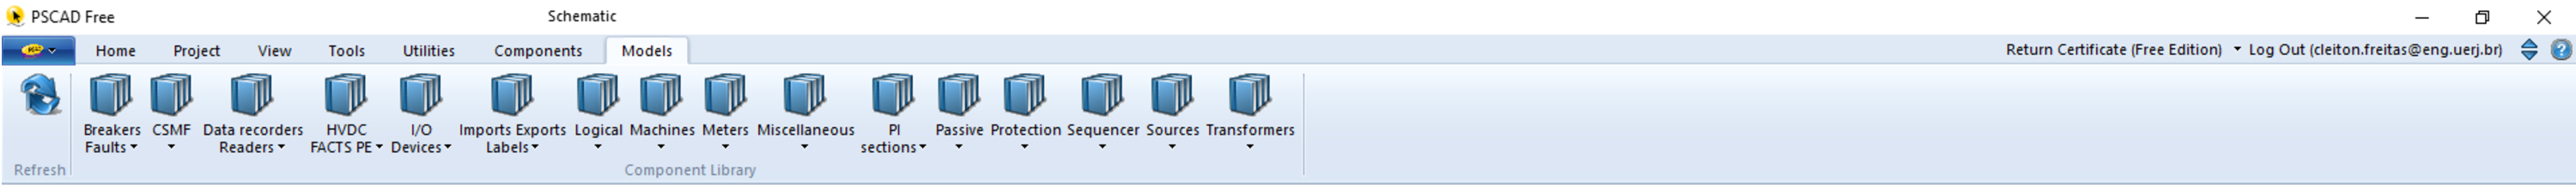
\includegraphics[width=0.85\linewidth]{./figuras/Primeiros-Passos/biblioteca_barra_models}

\end{frame}





%%%%%%%%%%%%%%%%%%%%%%%%%%%%%%%%%%%%%%%%%%%%%%%%
%%%%%%%%%%%%%%%%%%%%%%%%%%%%%%%%%%%%%%%%%%%%%%%%
%%%%%%%%%%%%%%%%%%%%%%%%%%%%%%%%%%%%%%%%%%%%%%%%
%%%%%%%%%%%%%%%%%%%%%%%%%%%%%%%%%%%%%%%%%%%%%%%%
\begin{frame}{Iniciando uma Simulação}
\centering

teste

\end{frame}






%%%%%%%%%%%%%%%%%%%%%%%%%%%%%%%%%%%%%%%%%%%%%%%%
%%%%%%%%%%%%%%%%%%%%%%%%%%%%%%%%%%%%%%%%%%%%%%%%
%%%%%%%%%%%%%%%%%%%%%%%%%%%%%%%%%%%%%%%%%%%%%%%%
%%%%%%%%%%%%%%%%%%%%%%%%%%%%%%%%%%%%%%%%%%%%%%%%
\begin{frame}{Configurações da Simulação}
\centering

teste

\end{frame}





%%%%%%%%%%%%%%%%%%%%%%%%%%%%%%%%%%%%%%%%%%%%%%%%
%%%%%%%%%%%%%%%%%%%%%%%%%%%%%%%%%%%%%%%%%%%%%%%%
%%%%%%%%%%%%%%%%%%%%%%%%%%%%%%%%%%%%%%%%%%%%%%%%
%%%%%%%%%%%%%%%%%%%%%%%%%%%%%%%%%%%%%%%%%%%%%%%%
\begin{frame}{Circuito Simulado}
\centering

teste

\end{frame}




\cmfnewsection{Visualização de Resultados: Alguns Detalhes}{./logos/fundo_tese}{0.15}




%%%%%%%%%%%%%%%%%%%%%%%%%%%%%%%%%%%%%%%%%%%%%%%%
%%%%%%%%%%%%%%%%%%%%%%%%%%%%%%%%%%%%%%%%%%%%%%%%
%%%%%%%%%%%%%%%%%%%%%%%%%%%%%%%%%%%%%%%%%%%%%%%%
%%%%%%%%%%%%%%%%%%%%%%%%%%%%%%%%%%%%%%%%%%%%%%%%
\begin{frame}{Ajustes nos Gráficos: Curvas}
\centering

\begin{columns}
\column{0.3\linewidth}

\begin{itemize}
\item É possível selecionar qual curva mostrar
\vspace*{2cm}
\item É possível selecionar aumentar a espessura da curva
\end{itemize}


\column{0.7\linewidth}
\centering
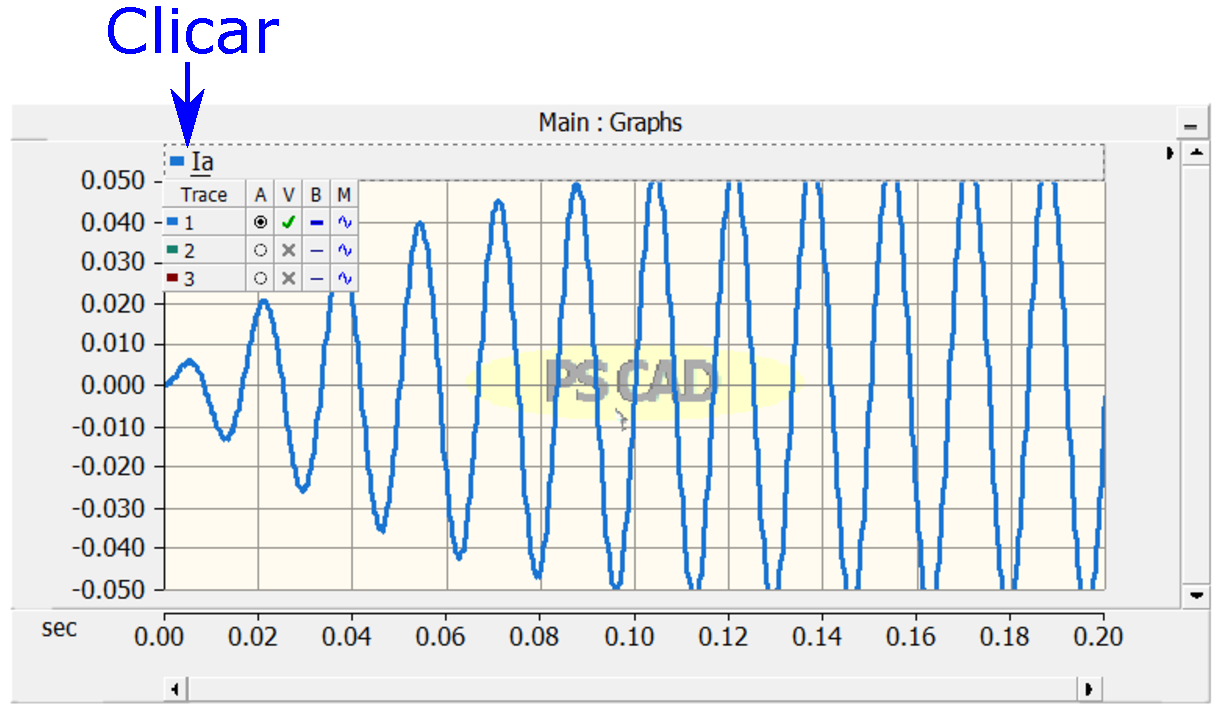
\includegraphics[width=0.9\linewidth]{./figuras/Visualizacao-resultados/graficos-Selecao}

\end{columns}

\end{frame}





%%%%%%%%%%%%%%%%%%%%%%%%%%%%%%%%%%%%%%%%%%%%%%%%
%%%%%%%%%%%%%%%%%%%%%%%%%%%%%%%%%%%%%%%%%%%%%%%%
%%%%%%%%%%%%%%%%%%%%%%%%%%%%%%%%%%%%%%%%%%%%%%%%
%%%%%%%%%%%%%%%%%%%%%%%%%%%%%%%%%%%%%%%%%%%%%%%%
\begin{frame}{Ajustes nos Gráficos: Escala}
\centering

\begin{columns}
\column{0.3\linewidth}

\begin{itemize}
\item Propriedades do gráfico
\vspace*{1cm}
\item Permite ajustar a escala
\vspace*{1cm}
\item Permite alterar a grade
\end{itemize}


\column{0.7\linewidth}
\centering
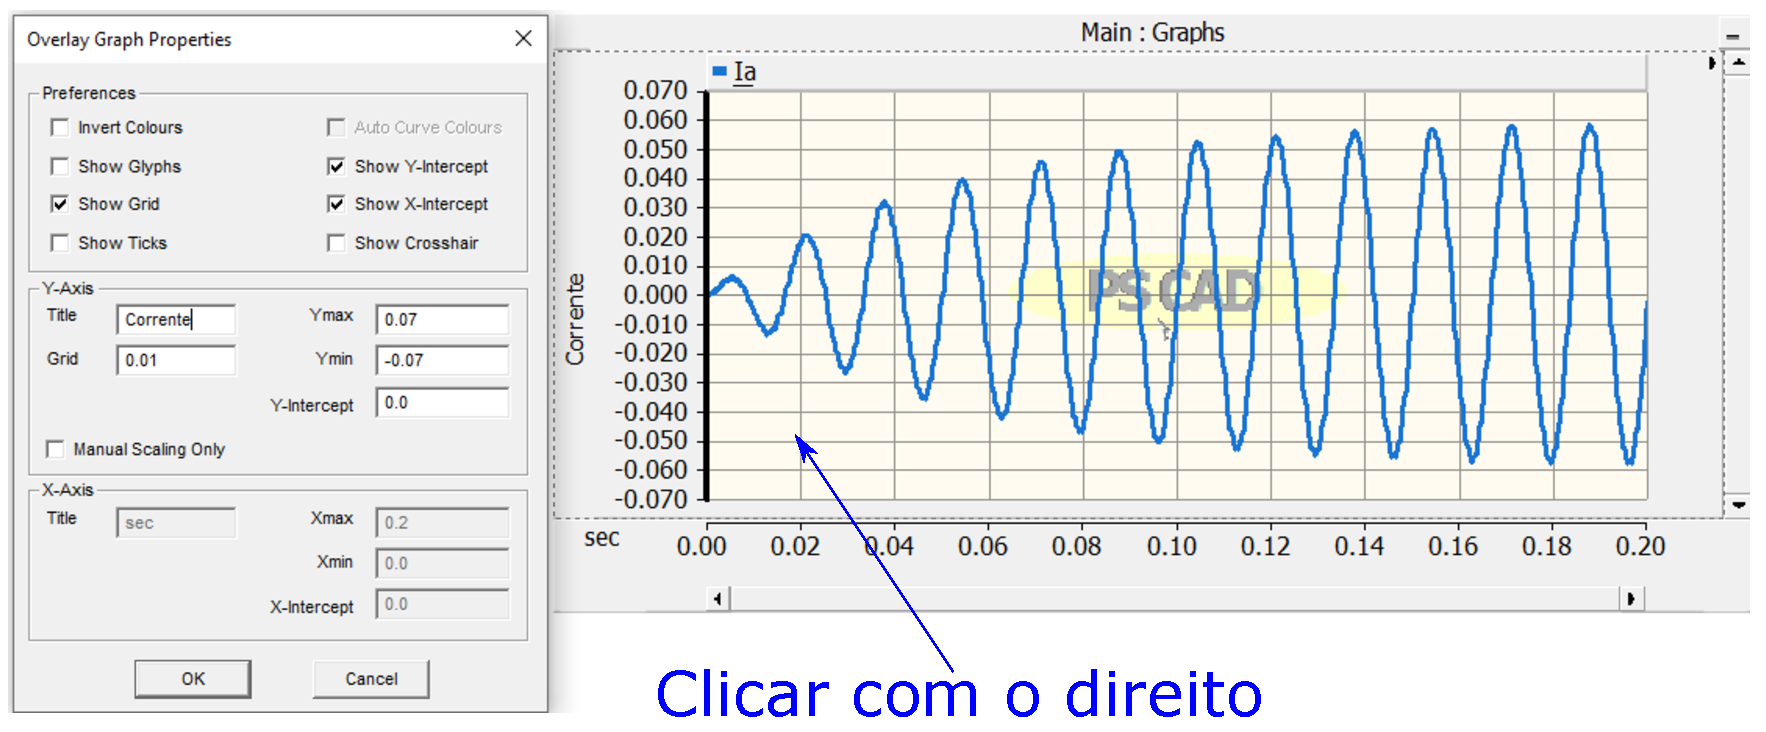
\includegraphics[width=0.9\linewidth]{./figuras/Visualizacao-resultados/graficos-escalas}

\end{columns}

\end{frame}





%%%%%%%%%%%%%%%%%%%%%%%%%%%%%%%%%%%%%%%%%%%%%%%%
%%%%%%%%%%%%%%%%%%%%%%%%%%%%%%%%%%%%%%%%%%%%%%%%
%%%%%%%%%%%%%%%%%%%%%%%%%%%%%%%%%%%%%%%%%%%%%%%%
%%%%%%%%%%%%%%%%%%%%%%%%%%%%%%%%%%%%%%%%%%%%%%%%
\begin{frame}{Ajustes nos Gráficos: Atalhos}

Depois de clicar no gráfico:
\vspace*{1cm}
\begin{itemize}
\item \textbf{E} - Ajusta a escala do tempo
\vspace*{0.75cm}
\item \textbf{Y} - Ajusta a escala y do gráfico para melhor visualização
\vspace*{0.75cm}
\item \textbf{B} - Ajusta a escala y do gráfico de acordo com a configuração do output chanel
\vspace*{0.75cm}
\item \textbf{M} - Habilita dois cursores 
\end{itemize}

\end{frame}




%%%%%%%%%%%%%%%%%%%%%%%%%%%%%%%%%%%%%%%%%%%%%%%%
%%%%%%%%%%%%%%%%%%%%%%%%%%%%%%%%%%%%%%%%%%%%%%%%
%%%%%%%%%%%%%%%%%%%%%%%%%%%%%%%%%%%%%%%%%%%%%%%%
%%%%%%%%%%%%%%%%%%%%%%%%%%%%%%%%%%%%%%%%%%%%%%%%
\begin{frame}{Ajustes nos Gráficos: Polygrphs}
\centering

\begin{columns}
\column{0.3\linewidth}

\begin{itemize}
\item Propriedades do gráfico
\vspace*{1cm}
\item Permite ajustar a escala
\vspace*{1cm}
\item Permite alterar a grade
\end{itemize}


\column{0.7\linewidth}
\centering
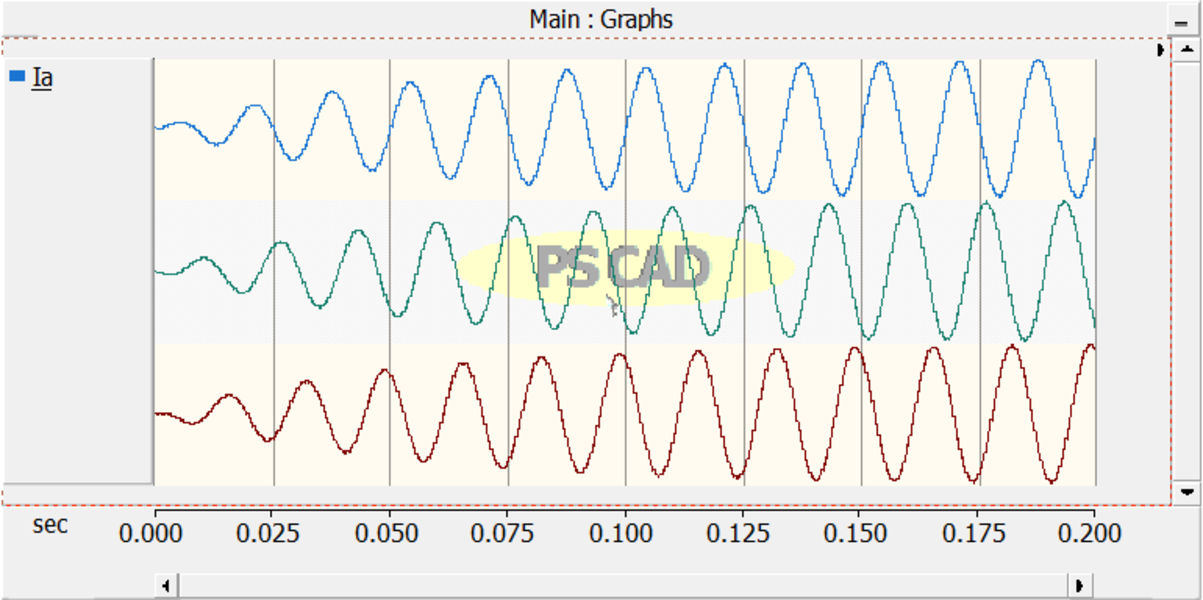
\includegraphics[width=0.9\linewidth]{./figuras/Visualizacao-resultados/graficos-polygraph}

\end{columns}

\end{frame}





%%%%%%%%%%%%%%%%%%%%%%%%%%%%%%%%%%%%%%%%%%%%%%%%
%%%%%%%%%%%%%%%%%%%%%%%%%%%%%%%%%%%%%%%%%%%%%%%%
%%%%%%%%%%%%%%%%%%%%%%%%%%%%%%%%%%%%%%%%%%%%%%%%
%%%%%%%%%%%%%%%%%%%%%%%%%%%%%%%%%%%%%%%%%%%%%%%%
\begin{frame}{Ajustes nos Gráficos: adicionando curvas ao gráfico}
\centering


\begin{columns}
\column{0.25\linewidth}

\begin{itemize}
\item Selecione o {\it output chanel}
\vspace*{1cm}
\item Precione a tecla {\it CTRL}
\vspace*{1cm}
\item Arraste em direção a um gráfico existente
\end{itemize}


\column{0.75\linewidth}
\centering
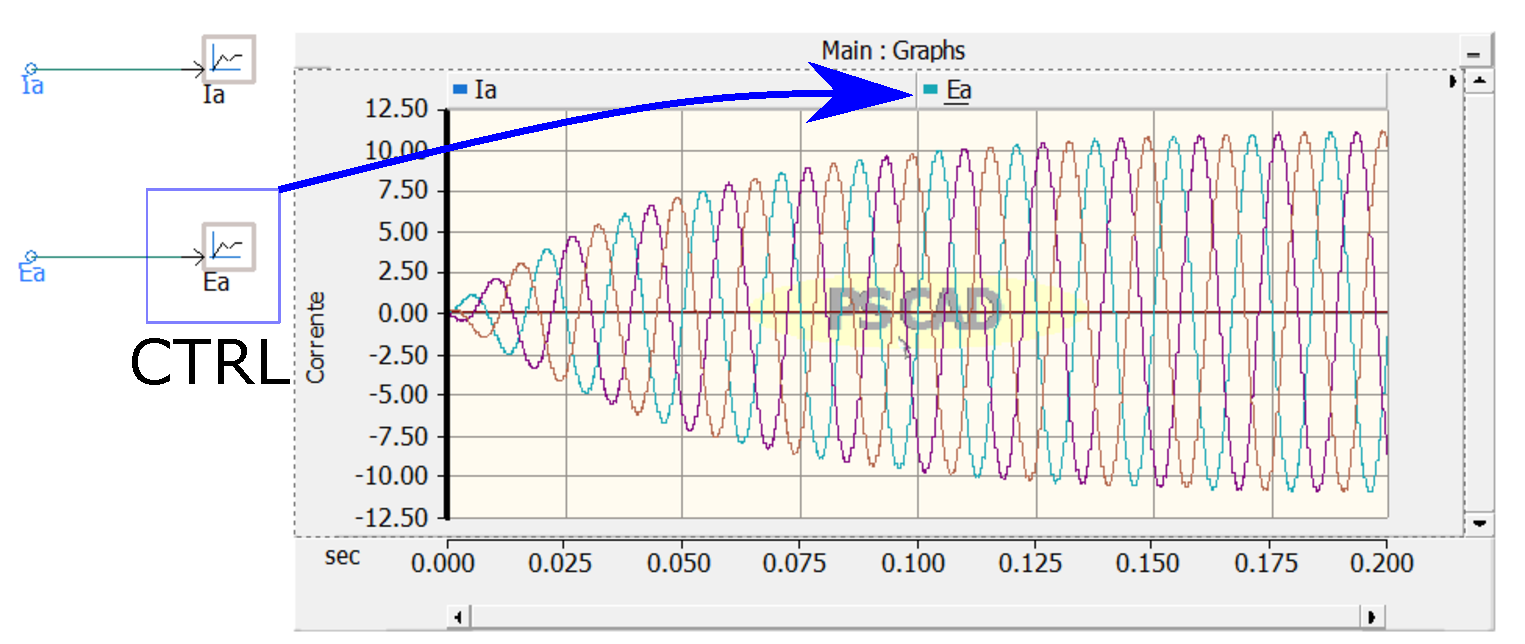
\includegraphics[width=0.95\linewidth]{./figuras/Visualizacao-resultados/graficos-add-curvas}

\end{columns}





\end{frame}






%%%%%%%%%%%%%%%%%%%%%%%%%%%%%%%%%%%%%%%%%%%%%%%%
%%%%%%%%%%%%%%%%%%%%%%%%%%%%%%%%%%%%%%%%%%%%%%%%
%%%%%%%%%%%%%%%%%%%%%%%%%%%%%%%%%%%%%%%%%%%%%%%%
%%%%%%%%%%%%%%%%%%%%%%%%%%%%%%%%%%%%%%%%%%%%%%%%
\begin{frame}{Ajustes nos Gráficos: Painéis de Controle}
\centering



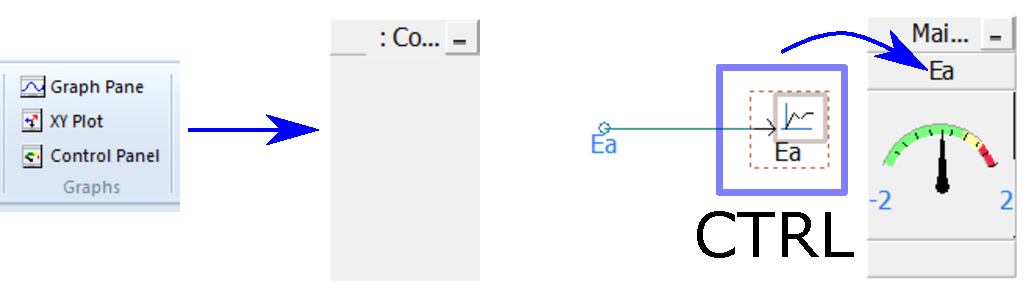
\includegraphics[width=0.95\linewidth]{./figuras/Visualizacao-resultados/graficos-Control-panel}




\end{frame}








%
%
%
%%%%%%%%%%%%%%%%%%%%%%%%%%%%%%%%%%%%%%%%%%%%%%%%%
%%%%%%%%%%%%%%%%%%%%%%%%%%%%%%%%%%%%%%%%%%%%%%%%%
%%%%%%%%%%%%%%%%%%%%%%%%%%%%%%%%%%%%%%%%%%%%%%%%%
%%%%%%%%%%%%%%%%%%%%%%%%%%%%%%%%%%%%%%%%%%%%%%%%%
%\begin{frame}{Ajustes nos Gráficos: Medidor Fasorial}
%\centering
%
%
%\end{frame}




\cmfnewsection{Circuitos Simples para Aprender Usar Outros Blocos}{./logos/fundo_tese}{0.15}








%%%%%%%%%%%%%%%%%%%%%%%%%%%%%%%%%%%%%%%%%%%%%%%%
%%%%%%%%%%%%%%%%%%%%%%%%%%%%%%%%%%%%%%%%%%%%%%%%
%%%%%%%%%%%%%%%%%%%%%%%%%%%%%%%%%%%%%%%%%%%%%%%%
%%%%%%%%%%%%%%%%%%%%%%%%%%%%%%%%%%%%%%%%%%%%%%%%
\begin{frame}{Circuito 2A}
\centering



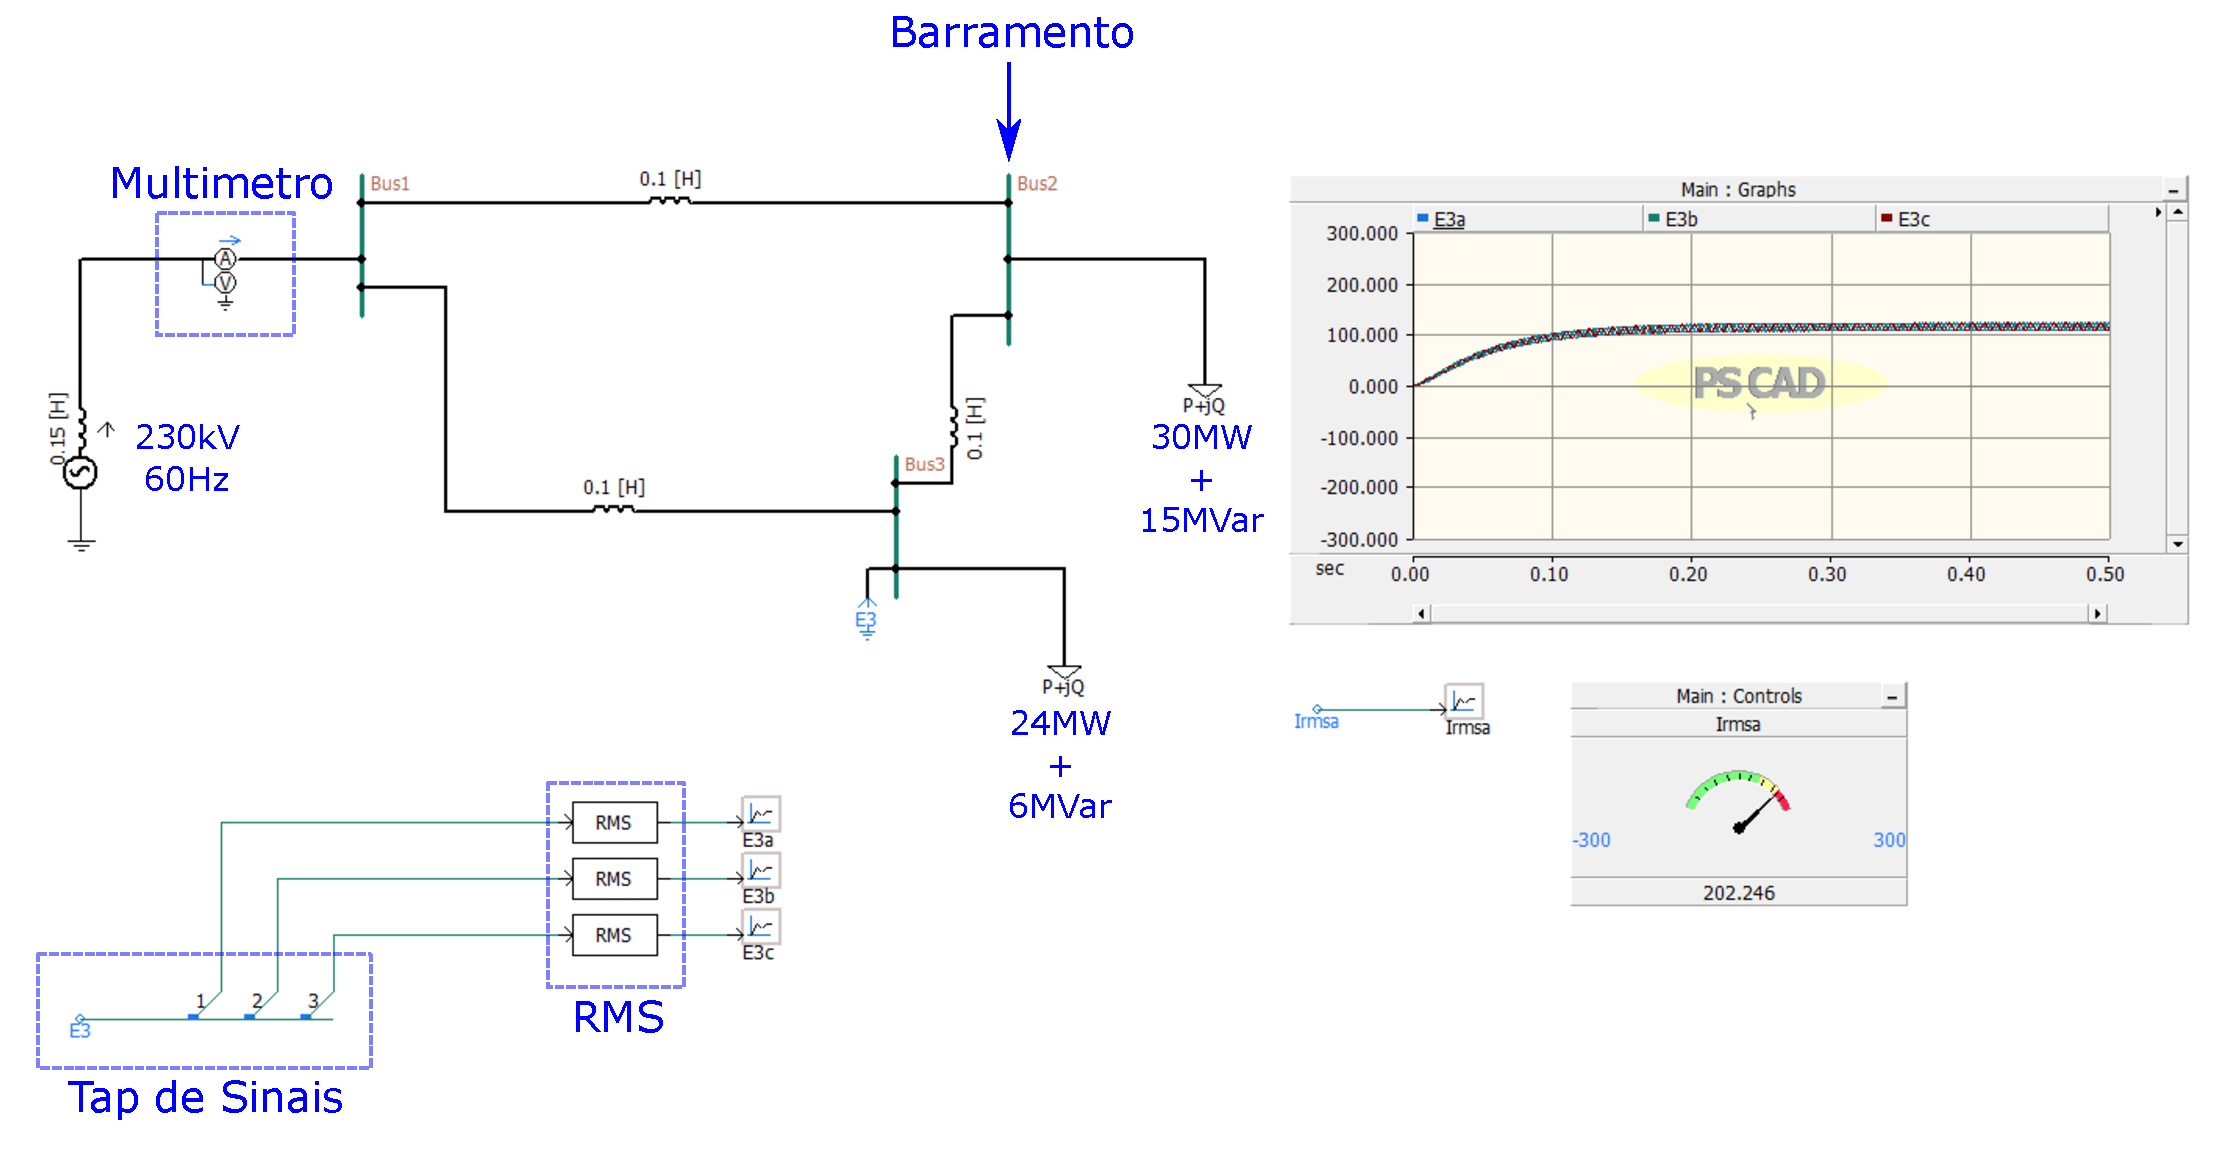
\includegraphics[width=0.95\linewidth]{./figuras/Segundo-Circuito/SIM2a}



\end{frame}






%%%%%%%%%%%%%%%%%%%%%%%%%%%%%%%%%%%%%%%%%%%%%%%%
%%%%%%%%%%%%%%%%%%%%%%%%%%%%%%%%%%%%%%%%%%%%%%%%
%%%%%%%%%%%%%%%%%%%%%%%%%%%%%%%%%%%%%%%%%%%%%%%%
%%%%%%%%%%%%%%%%%%%%%%%%%%%%%%%%%%%%%%%%%%%%%%%%
\begin{frame}{Circuito 2B}
\centering



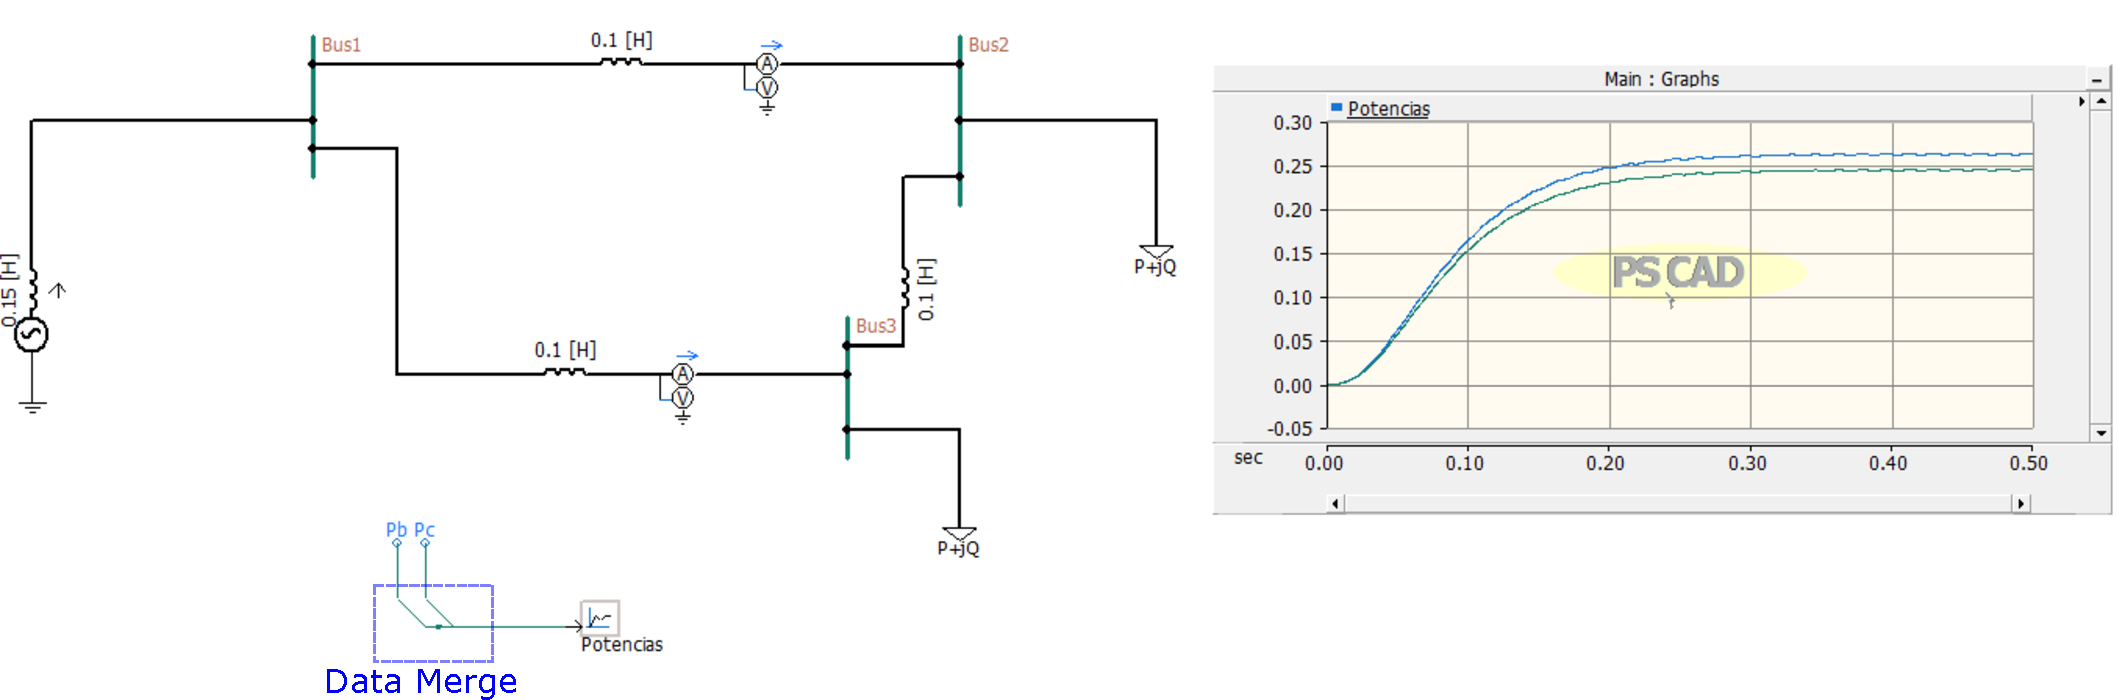
\includegraphics[width=0.95\linewidth]{./figuras/Segundo-Circuito/SIM2b}



\end{frame}







%%%%%%%%%%%%%%%%%%%%%%%%%%%%%%%%%%%%%%%%%%%%%%%%
%%%%%%%%%%%%%%%%%%%%%%%%%%%%%%%%%%%%%%%%%%%%%%%%
%%%%%%%%%%%%%%%%%%%%%%%%%%%%%%%%%%%%%%%%%%%%%%%%
%%%%%%%%%%%%%%%%%%%%%%%%%%%%%%%%%%%%%%%%%%%%%%%%
\begin{frame}{Circuito 2C}
\centering



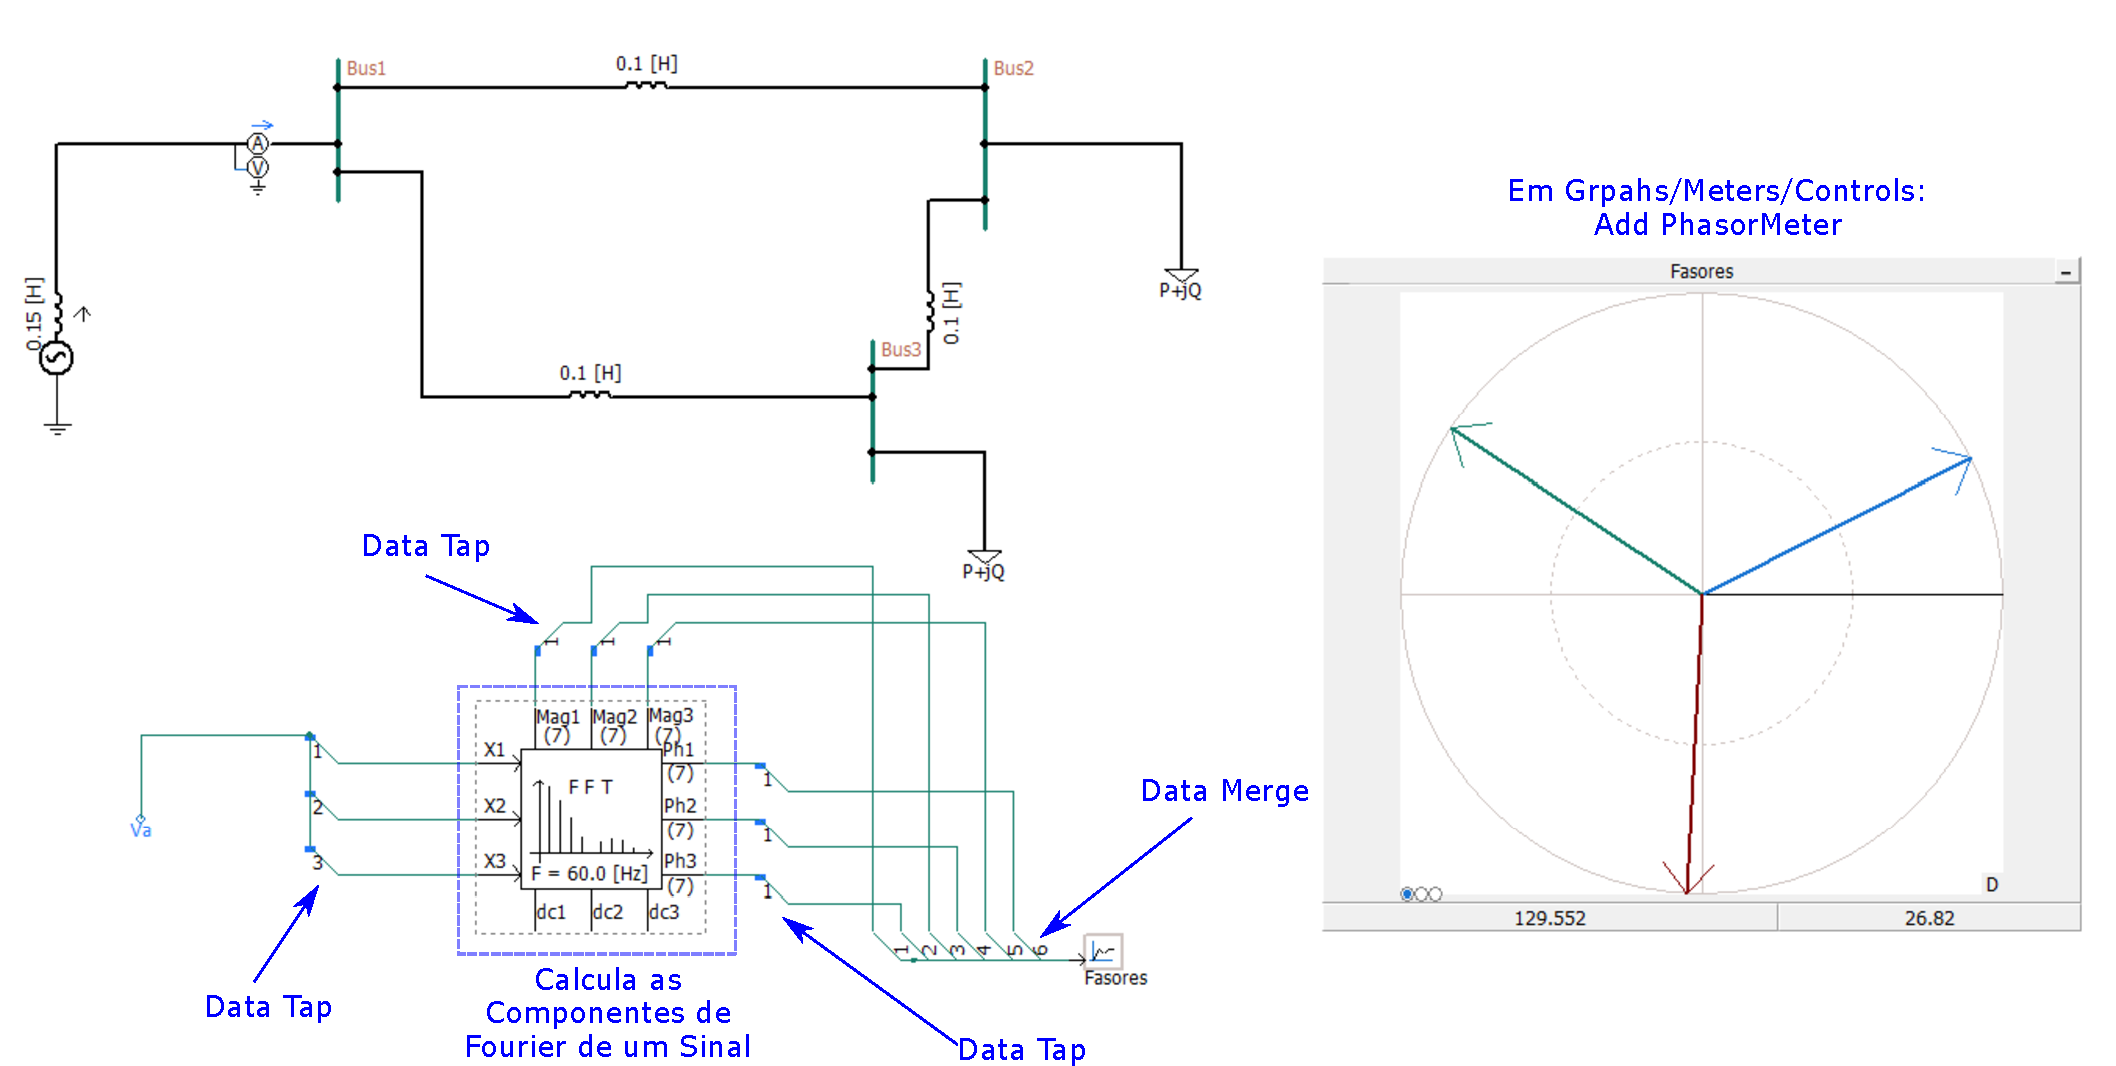
\includegraphics[width=0.95\linewidth]{./figuras/Segundo-Circuito/SIM2c}



\end{frame}







%%%%%%%%%%%%%%%%%%%%%%%%%%%%%%%%%%%%%%%%%%%%%%%%
%%%%%%%%%%%%%%%%%%%%%%%%%%%%%%%%%%%%%%%%%%%%%%%%
%%%%%%%%%%%%%%%%%%%%%%%%%%%%%%%%%%%%%%%%%%%%%%%%
%%%%%%%%%%%%%%%%%%%%%%%%%%%%%%%%%%%%%%%%%%%%%%%%
\begin{frame}{Circuito 2D: Nosso primeiro circuito monofásico}
\centering



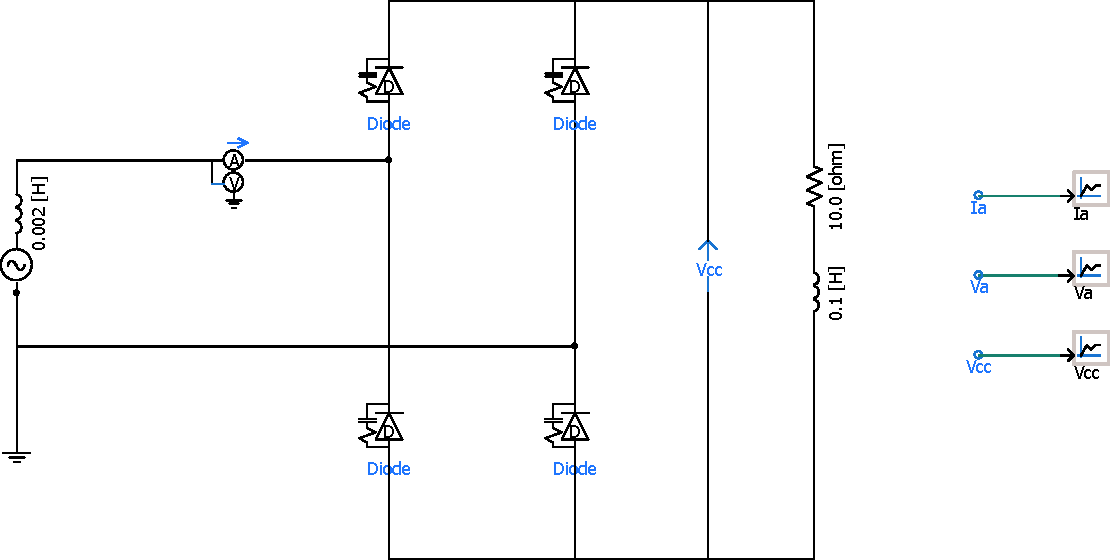
\includegraphics[width=0.75\linewidth]{./figuras/Segundo-Circuito/SIM2d}



\end{frame}






%%%%%%%%%%%%%%%%%%%%%%%%%%%%%%%%%%%%%%%%%%%%%%%%
%%%%%%%%%%%%%%%%%%%%%%%%%%%%%%%%%%%%%%%%%%%%%%%%
%%%%%%%%%%%%%%%%%%%%%%%%%%%%%%%%%%%%%%%%%%%%%%%%
%%%%%%%%%%%%%%%%%%%%%%%%%%%%%%%%%%%%%%%%%%%%%%%%
\begin{frame}{Circuito 2D: FFT}
\centering


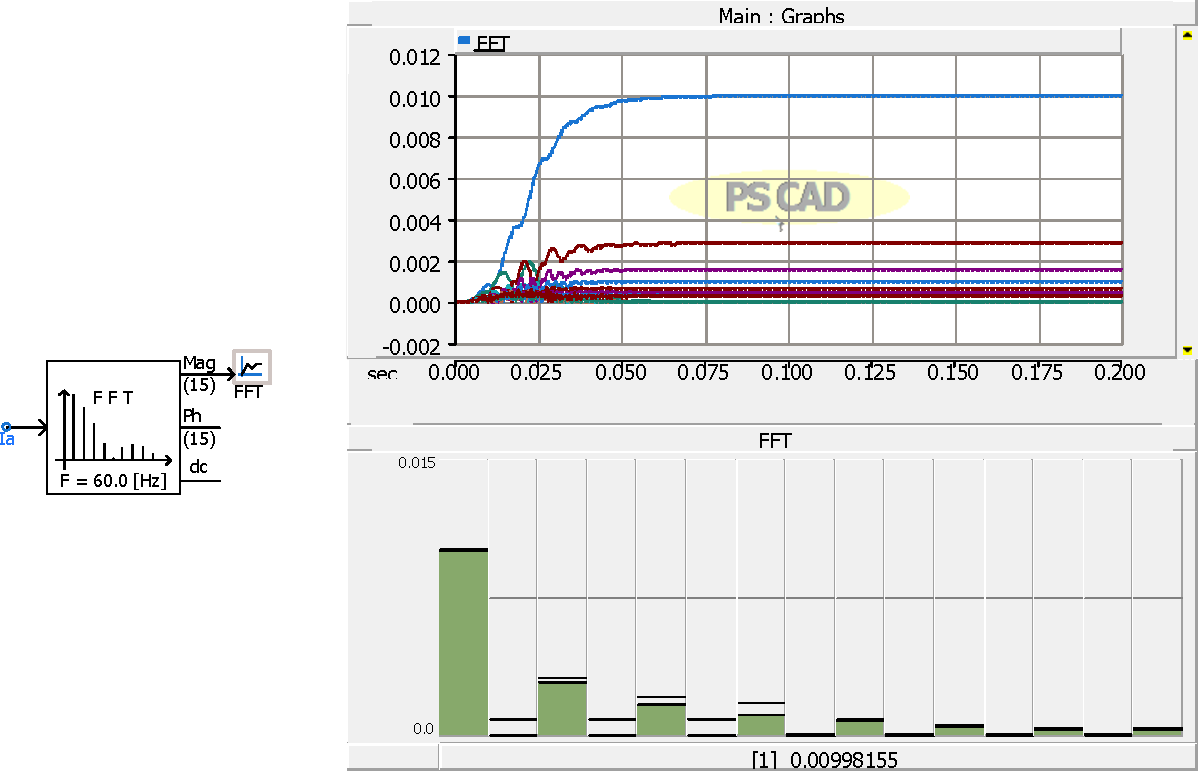
\includegraphics[width=0.70\linewidth]{./figuras/Segundo-Circuito/SIM2d-FFT}

\end{frame}




%%%%%%%%%%%%%%%%%%%%%%%%%%%%%%%%%%%%%%%%%%%%%%%%
%%%%%%%%%%%%%%%%%%%%%%%%%%%%%%%%%%%%%%%%%%%%%%%%
%%%%%%%%%%%%%%%%%%%%%%%%%%%%%%%%%%%%%%%%%%%%%%%%
%%%%%%%%%%%%%%%%%%%%%%%%%%%%%%%%%%%%%%%%%%%%%%%%
\begin{frame}{Circuito 2E: Transformadores e etc}
\centering


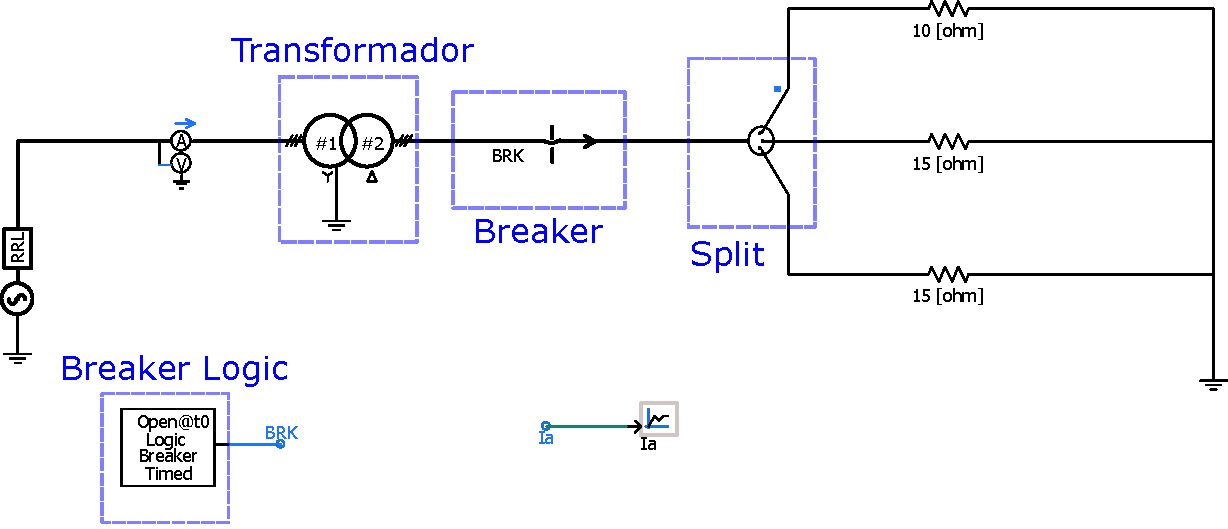
\includegraphics[width=0.70\linewidth]{./figuras/Segundo-Circuito/SIM2e}

\end{frame}






%%%%%%%%%%%%%%%%%%%%%%%%%%%%%%%%%%%%%%%%%%%%%%%%
%%%%%%%%%%%%%%%%%%%%%%%%%%%%%%%%%%%%%%%%%%%%%%%%
%%%%%%%%%%%%%%%%%%%%%%%%%%%%%%%%%%%%%%%%%%%%%%%%
%%%%%%%%%%%%%%%%%%%%%%%%%%%%%%%%%%%%%%%%%%%%%%%%
\begin{frame}{Circuito 2F: Máquinas CC}
\centering


\begin{columns}

\column{0.4\linewidth}
\centering
Máquina
\vspace*{0.5cm}

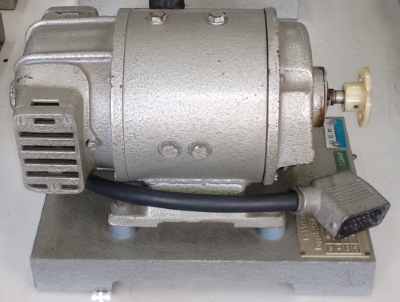
\includegraphics[width=0.95\linewidth]{./figuras/Segundo-Circuito/maquina_CC_b}

\column{0.6\linewidth}
\centering
Modelo Matemático\footnote[frame]{\tiny Stephen J. Chapman, Fundamentos das Máquinas Elétricas. 5ed. Capítulos 7 e 8.}
\vspace*{1cm}

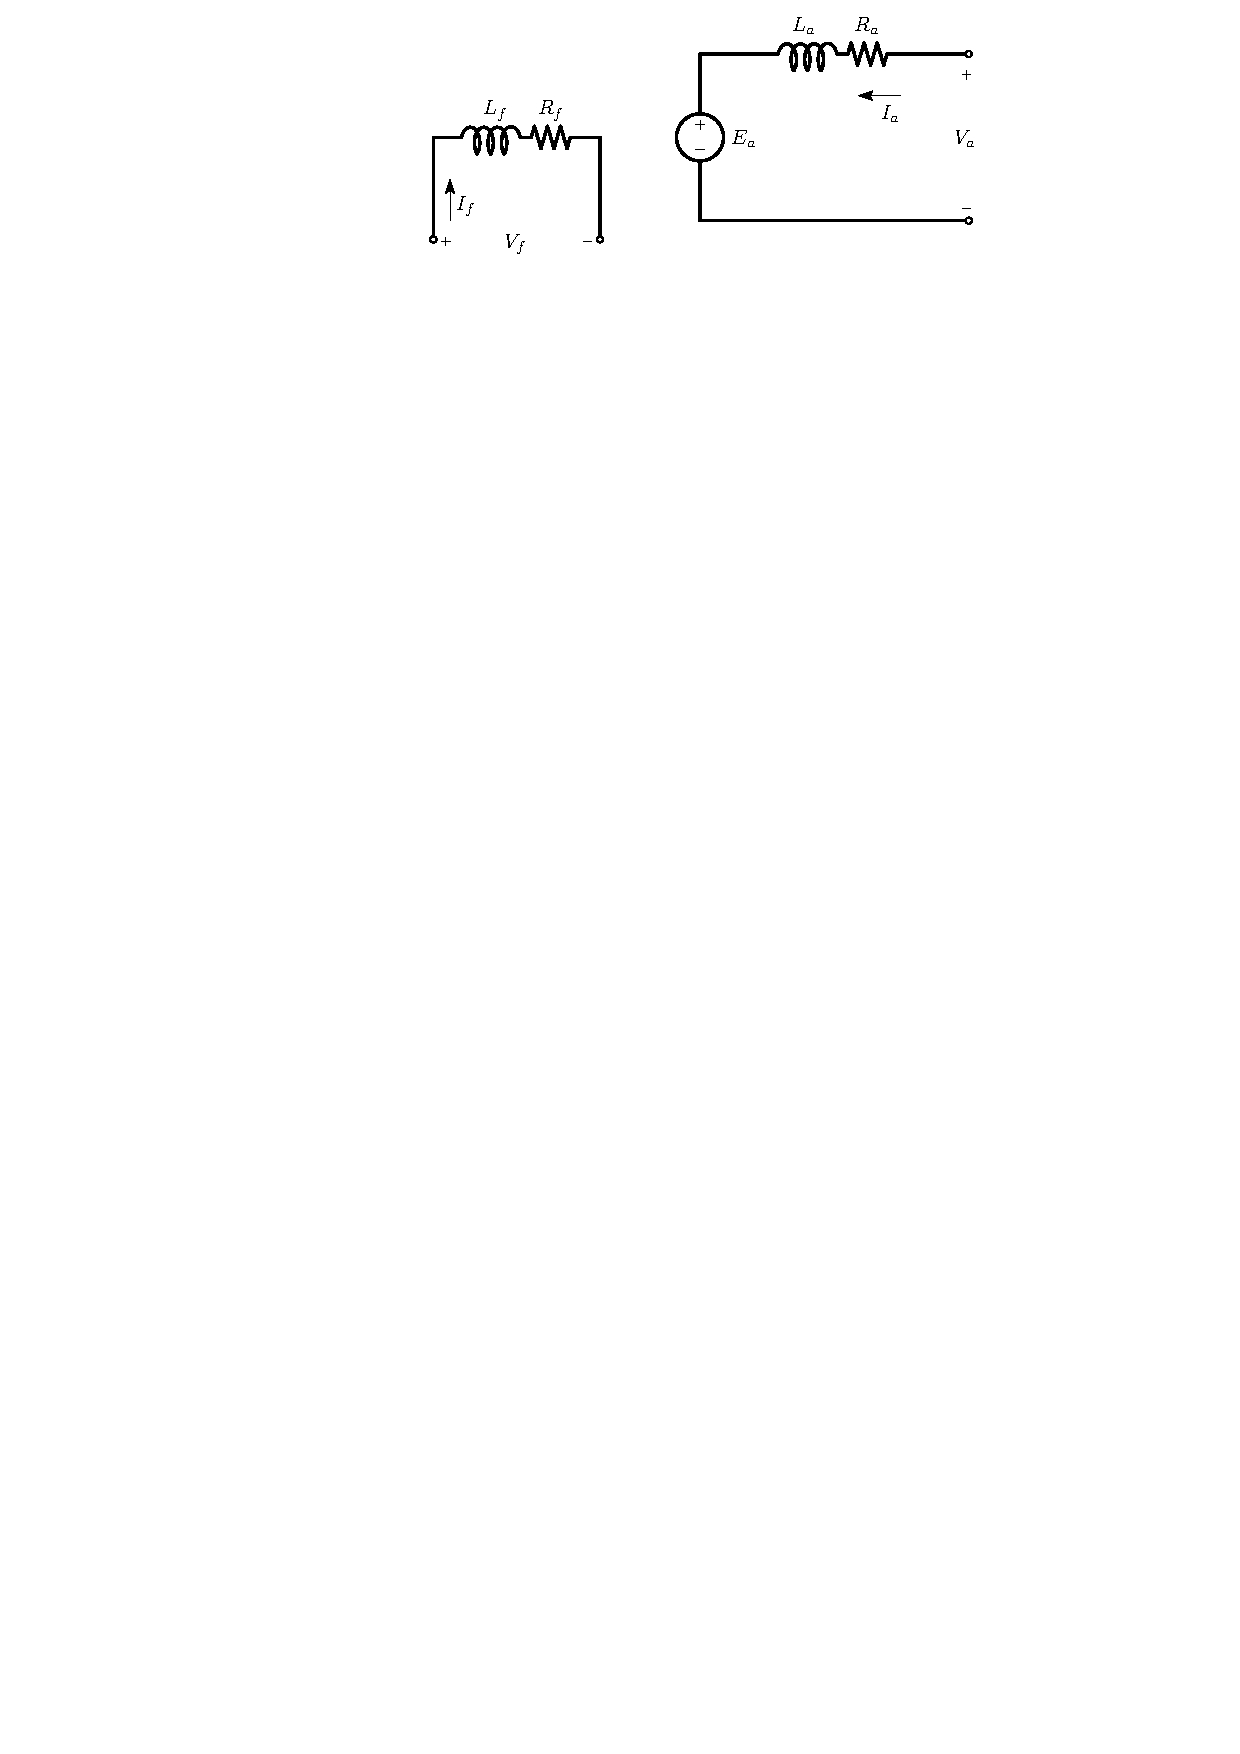
\includegraphics[width=0.95\linewidth]{./figuras/Segundo-Circuito/SIMf_dc_machine}

\end{columns}

\end{frame}





%%%%%%%%%%%%%%%%%%%%%%%%%%%%%%%%%%%%%%%%%%%%%%%%
%%%%%%%%%%%%%%%%%%%%%%%%%%%%%%%%%%%%%%%%%%%%%%%%
%%%%%%%%%%%%%%%%%%%%%%%%%%%%%%%%%%%%%%%%%%%%%%%%
%%%%%%%%%%%%%%%%%%%%%%%%%%%%%%%%%%%%%%%%%%%%%%%%
\begin{frame}{Circuito 2F: Mais Sobre o Modelo da Máquina}
\centering


\begin{columns}



\column{0.25\linewidth}
\centering

{\color{blue}Movimento

+

Fluxo  Magnético

$\downarrow$ 

Tensão Induzida
}





\column{0.5\linewidth}
\centering


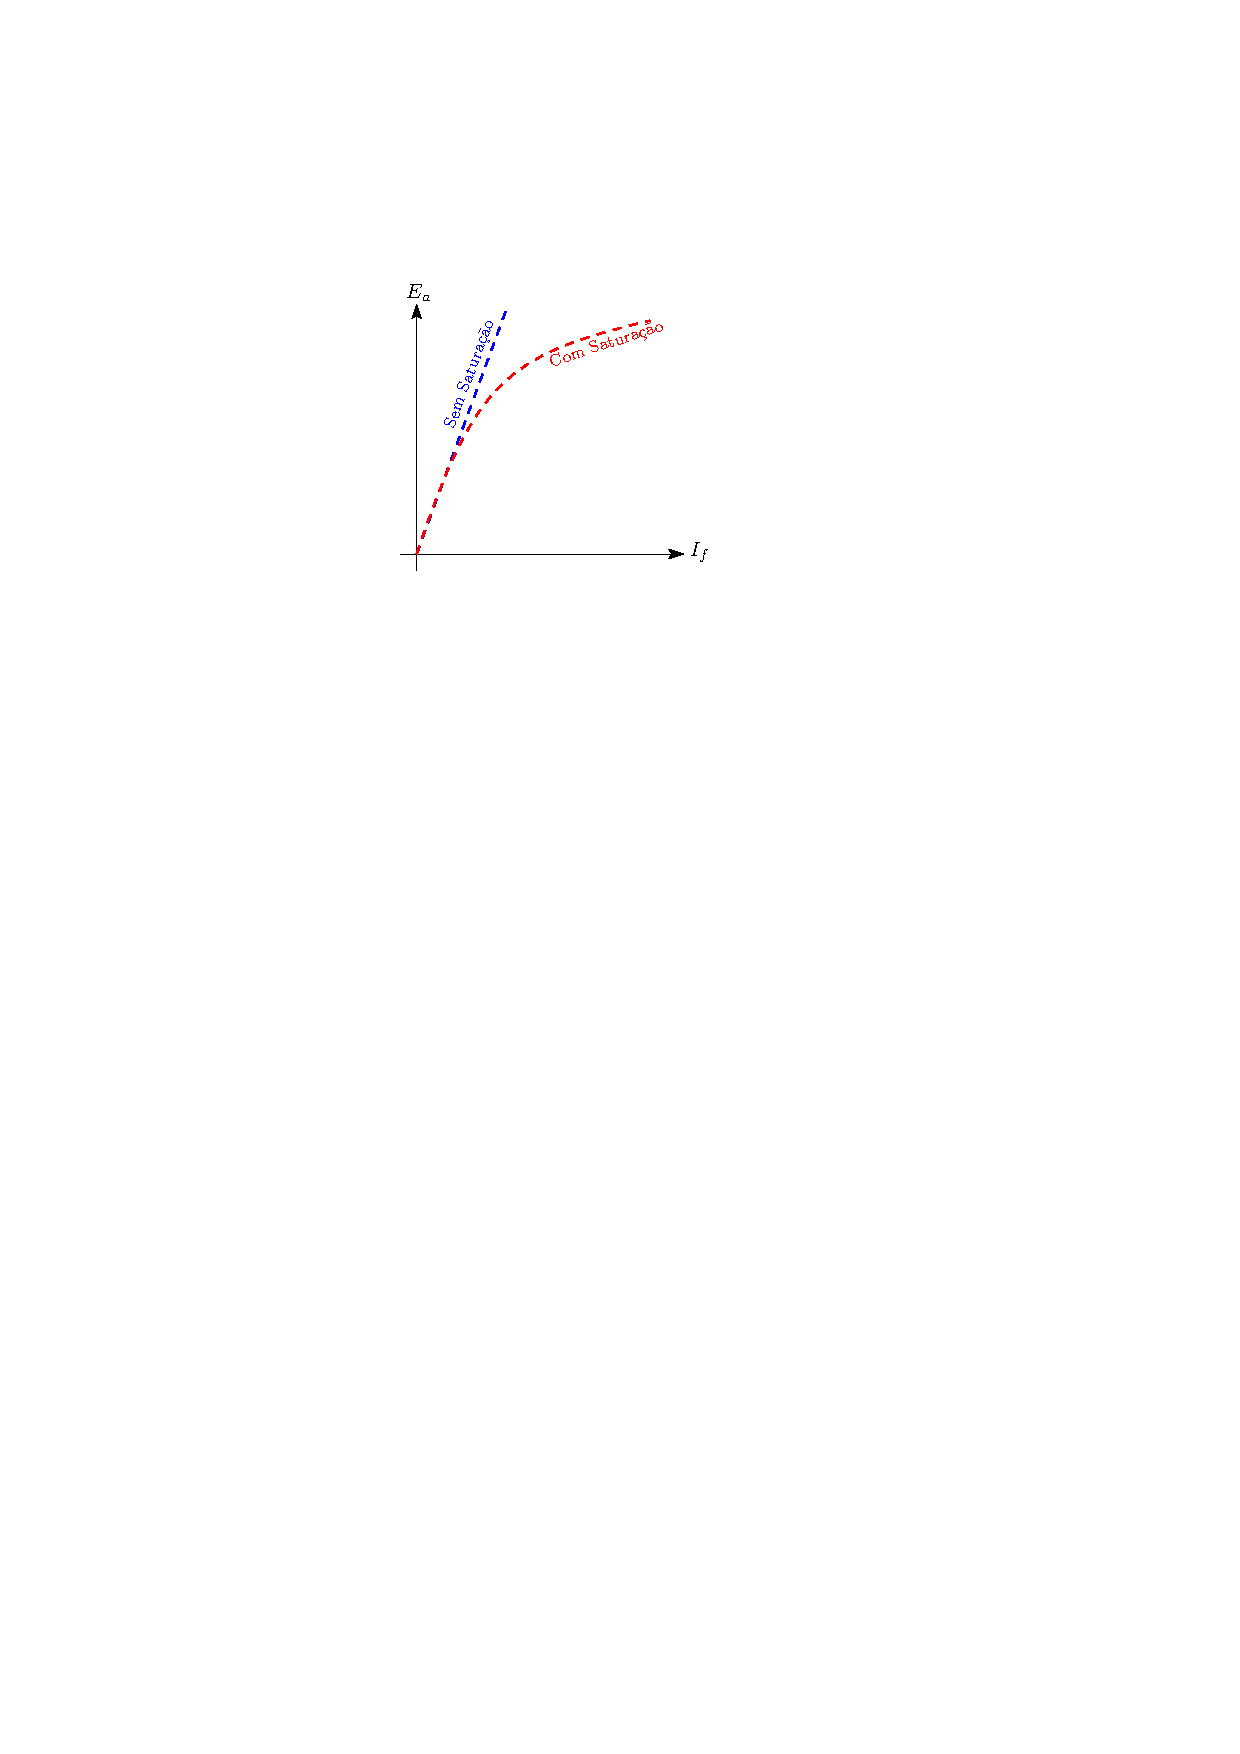
\includegraphics[width=0.85\linewidth]{./figuras/Segundo-Circuito/SIMf_dc_machine_excitation}




\column{0.25\linewidth}
\centering

{\color{blue}Corrente

+

Fluxo  Magnético

$\downarrow$ 

Torque
}

\end{columns}
\end{frame}




%%%%%%%%%%%%%%%%%%%%%%%%%%%%%%%%%%%%%%%%%%%%%%%%
%%%%%%%%%%%%%%%%%%%%%%%%%%%%%%%%%%%%%%%%%%%%%%%%
%%%%%%%%%%%%%%%%%%%%%%%%%%%%%%%%%%%%%%%%%%%%%%%%
%%%%%%%%%%%%%%%%%%%%%%%%%%%%%%%%%%%%%%%%%%%%%%%%
\begin{frame}{Circuito 2F: Máquinas CC no PSCAD}
\centering


\begin{columns}

\column{0.4\linewidth}
\centering

\begin{itemize}
\item Representa apenas as equações elétricas 
\vspace*{2cm}
\item A dinâmica mecânica é deixada de lado
\end{itemize}

\column{0.6\linewidth}
\centering


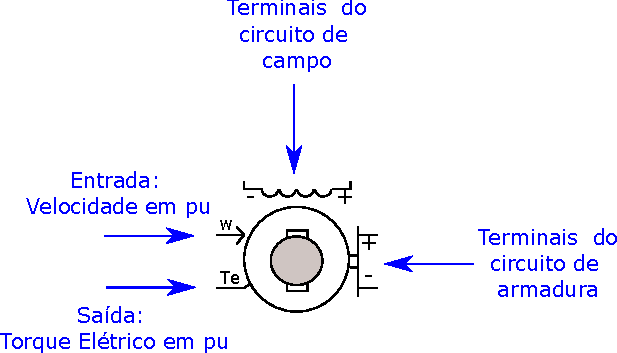
\includegraphics[width=0.95\linewidth]{./figuras/Segundo-Circuito/SEMf_maq_cc_pascad}

\end{columns}
\end{frame}




%%%%%%%%%%%%%%%%%%%%%%%%%%%%%%%%%%%%%%%%%%%%%%%%
%%%%%%%%%%%%%%%%%%%%%%%%%%%%%%%%%%%%%%%%%%%%%%%%
%%%%%%%%%%%%%%%%%%%%%%%%%%%%%%%%%%%%%%%%%%%%%%%%
%%%%%%%%%%%%%%%%%%%%%%%%%%%%%%%%%%%%%%%%%%%%%%%%
\begin{frame}{Circuito 2F: Modelando a Dinâmica Mecânica}
\centering


\begin{columns}

\column{0.5\linewidth}

{\it Lei de Newton} dos sistemas rotacionais:
\begin{equation*}
J \frac{d \omega_m}{dt} = T_e - T_m 
\end{equation*}



\column{0.5\linewidth}

Convertendo para pu: 
\begin{equation*}
2 H \frac{d \omega_{m,pu}}{dt}  = T_{e,pu} - T_{m,pu} 
\end{equation*}




\end{columns}

\begin{equation*}
H = \frac{J}{2}  \frac{\omega_{nominal}}{P_{nominal}}
\end{equation*}

\begin{itemize}
\item $T_e$ - Torque eletromagnético (calculado pelo modelo da máquina)
\item $T_m$ - Torque mecânico 
\item $\omega_m$ - Velocidade mecânica
\end{itemize}

\end{frame}







%%%%%%%%%%%%%%%%%%%%%%%%%%%%%%%%%%%%%%%%%%%%%%%%
%%%%%%%%%%%%%%%%%%%%%%%%%%%%%%%%%%%%%%%%%%%%%%%%
%%%%%%%%%%%%%%%%%%%%%%%%%%%%%%%%%%%%%%%%%%%%%%%%
%%%%%%%%%%%%%%%%%%%%%%%%%%%%%%%%%%%%%%%%%%%%%%%%
\begin{frame}{Circuito 2F: Circuito}
\centering

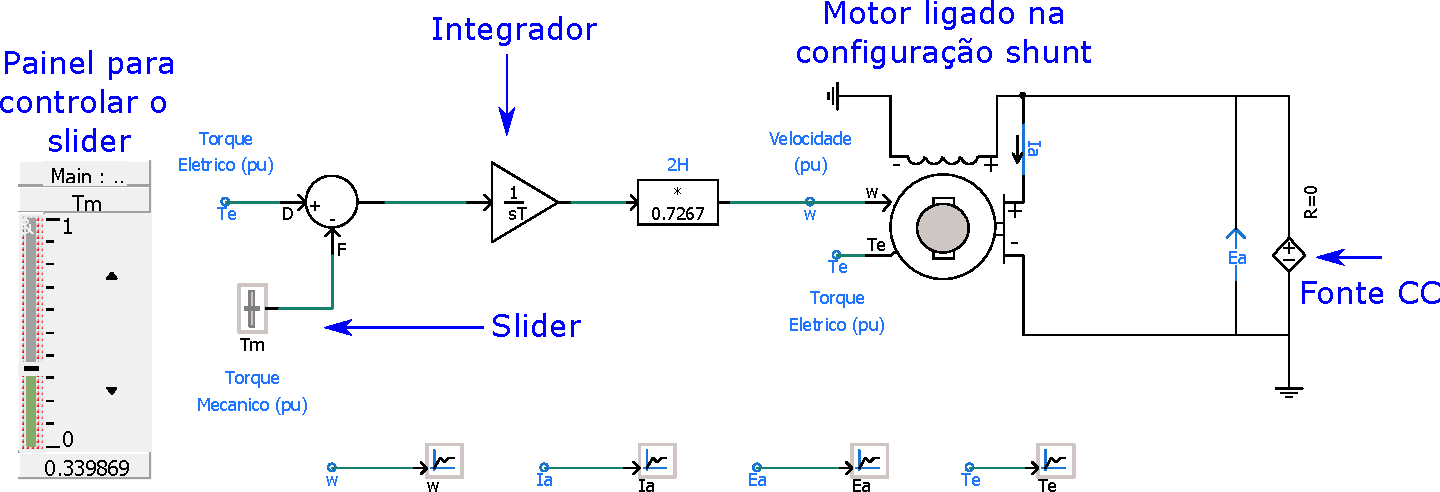
\includegraphics[width=0.9\linewidth]{./figuras/Segundo-Circuito/SIM2f}

\end{frame}
\cmfnewsection{Mais Simulações}{./logos/fundo_tese}{0.15}






%%%%%%%%%%%%%%%%%%%%%%%%%%%%%%%%%%%%%%%%%%%%%%%%
%%%%%%%%%%%%%%%%%%%%%%%%%%%%%%%%%%%%%%%%%%%%%%%%
%%%%%%%%%%%%%%%%%%%%%%%%%%%%%%%%%%%%%%%%%%%%%%%%
%%%%%%%%%%%%%%%%%%%%%%%%%%%%%%%%%%%%%%%%%%%%%%%%
\begin{frame}{Circuito A: Inversor {\it Stand alone}}
\centering


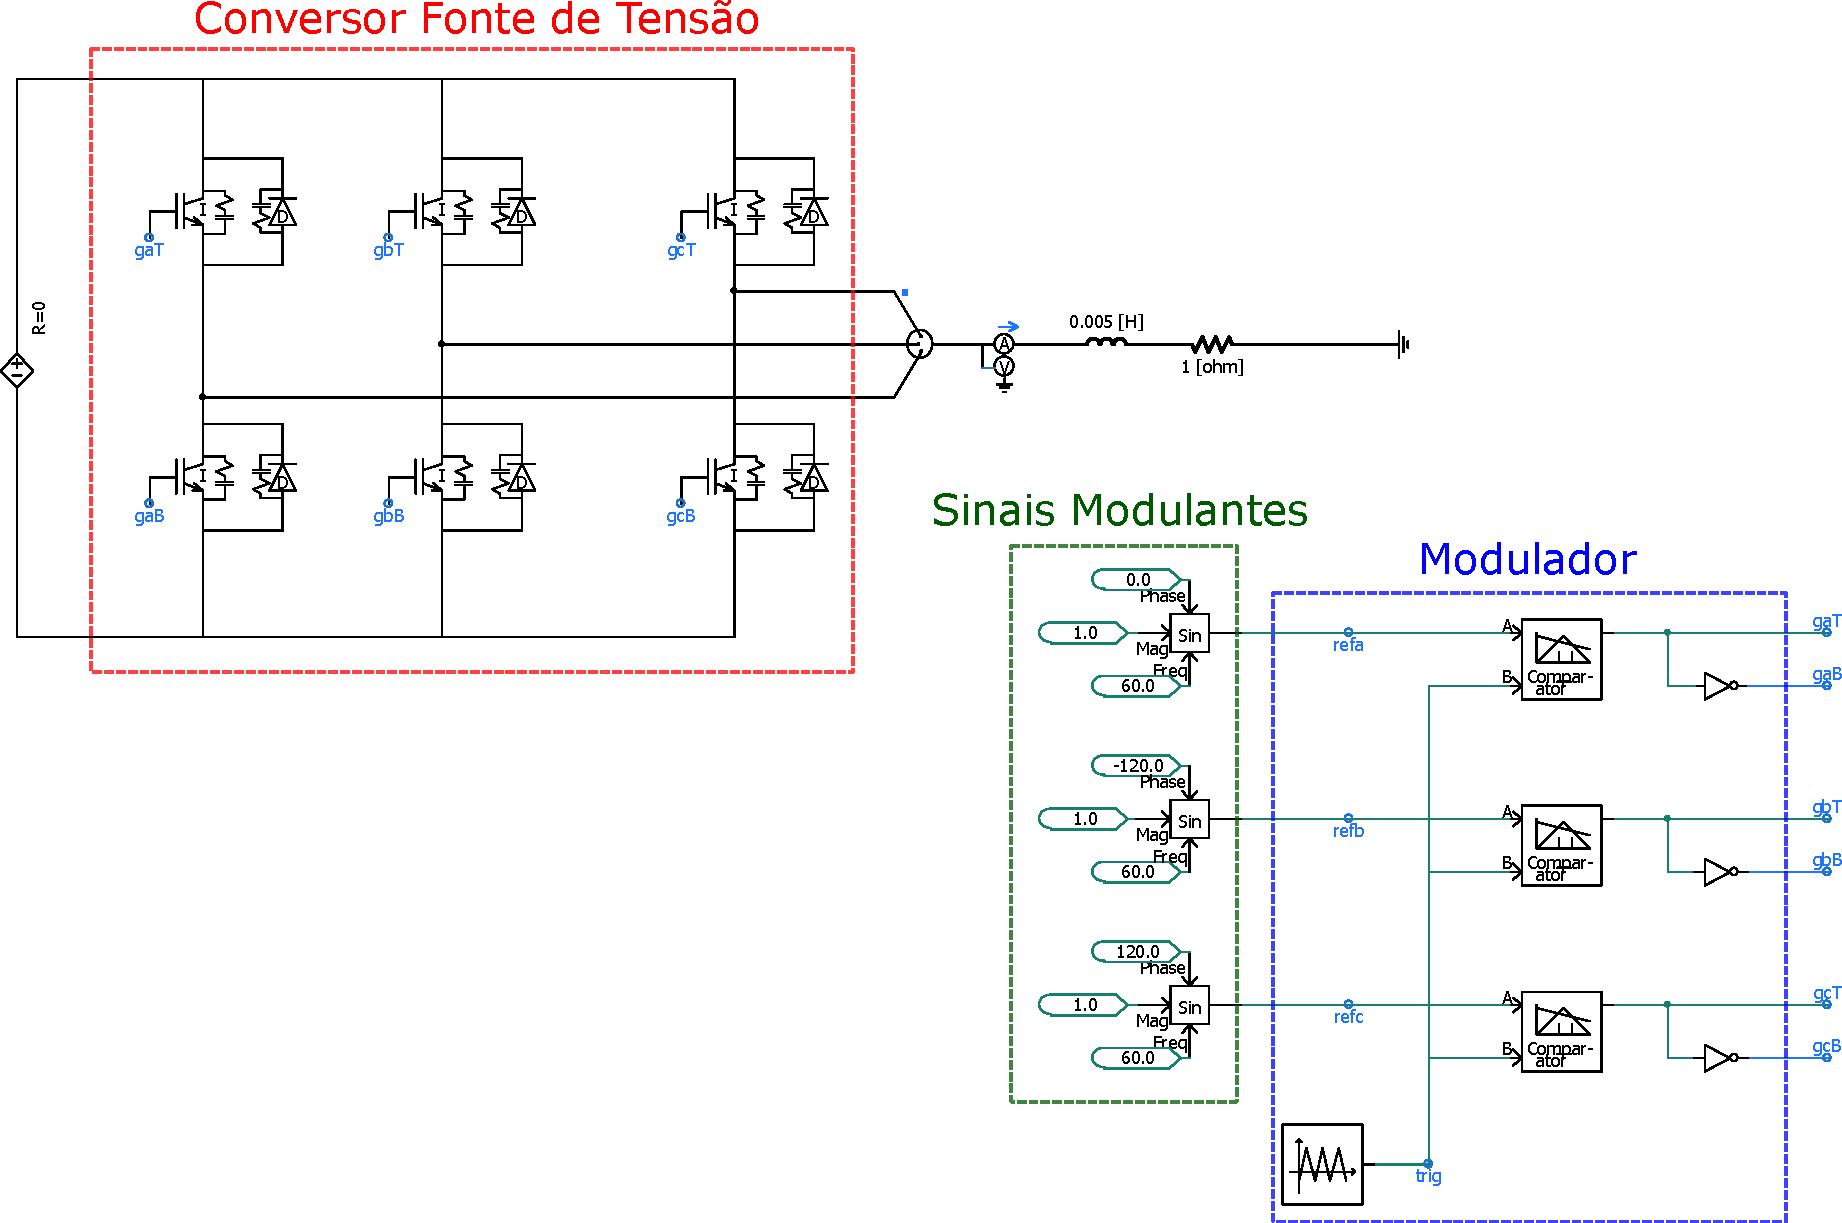
\includegraphics[width=0.65\linewidth]{./figuras/Terceiro-Circuito/SIM6a}


\end{frame}








%%%%%%%%%%%%%%%%%%%%%%%%%%%%%%%%%%%%%%%%%%%%%%%%
%%%%%%%%%%%%%%%%%%%%%%%%%%%%%%%%%%%%%%%%%%%%%%%%
%%%%%%%%%%%%%%%%%%%%%%%%%%%%%%%%%%%%%%%%%%%%%%%%
%%%%%%%%%%%%%%%%%%%%%%%%%%%%%%%%%%%%%%%%%%%%%%%%
\begin{frame}{Circuito B: Inversor Conectado a Rede}
\centering


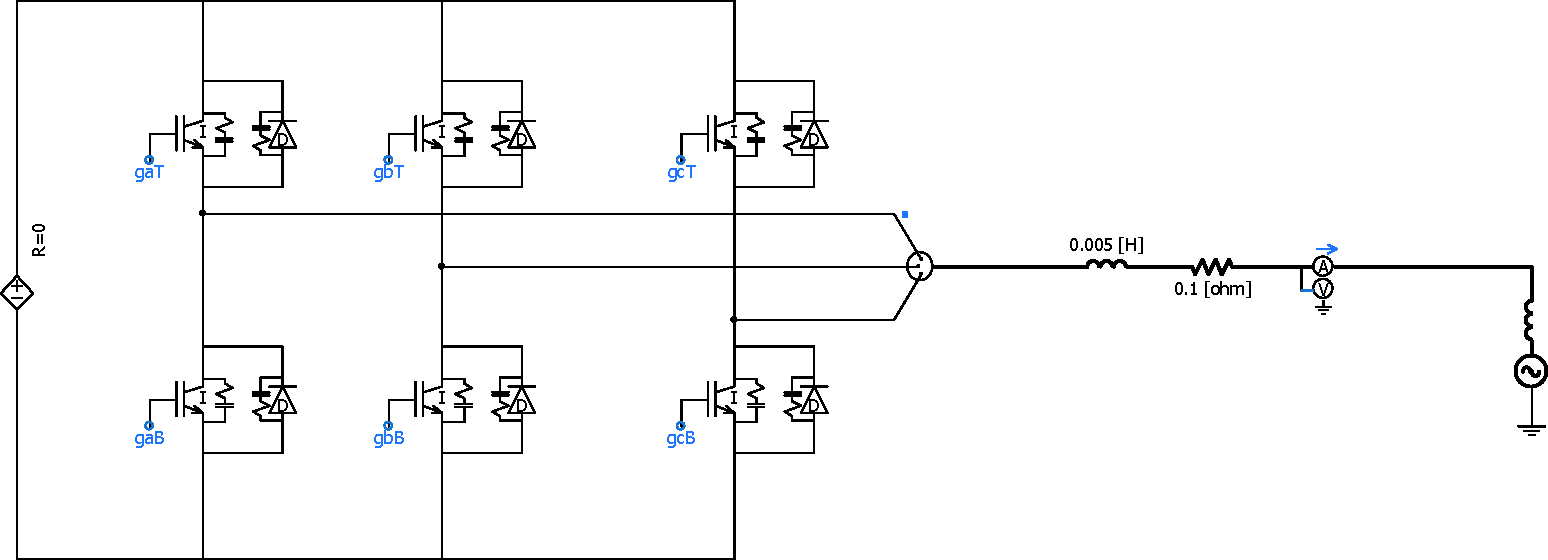
\includegraphics[width=0.75\linewidth]{./figuras/Terceiro-Circuito/SIM6b_CIRCUITO}


\end{frame}




%%%%%%%%%%%%%%%%%%%%%%%%%%%%%%%%%%%%%%%%%%%%%%%%
%%%%%%%%%%%%%%%%%%%%%%%%%%%%%%%%%%%%%%%%%%%%%%%%
%%%%%%%%%%%%%%%%%%%%%%%%%%%%%%%%%%%%%%%%%%%%%%%%
%%%%%%%%%%%%%%%%%%%%%%%%%%%%%%%%%%%%%%%%%%%%%%%%
\begin{frame}{Circuito B: Inversor Conectado a Rede - Controle}
\centering


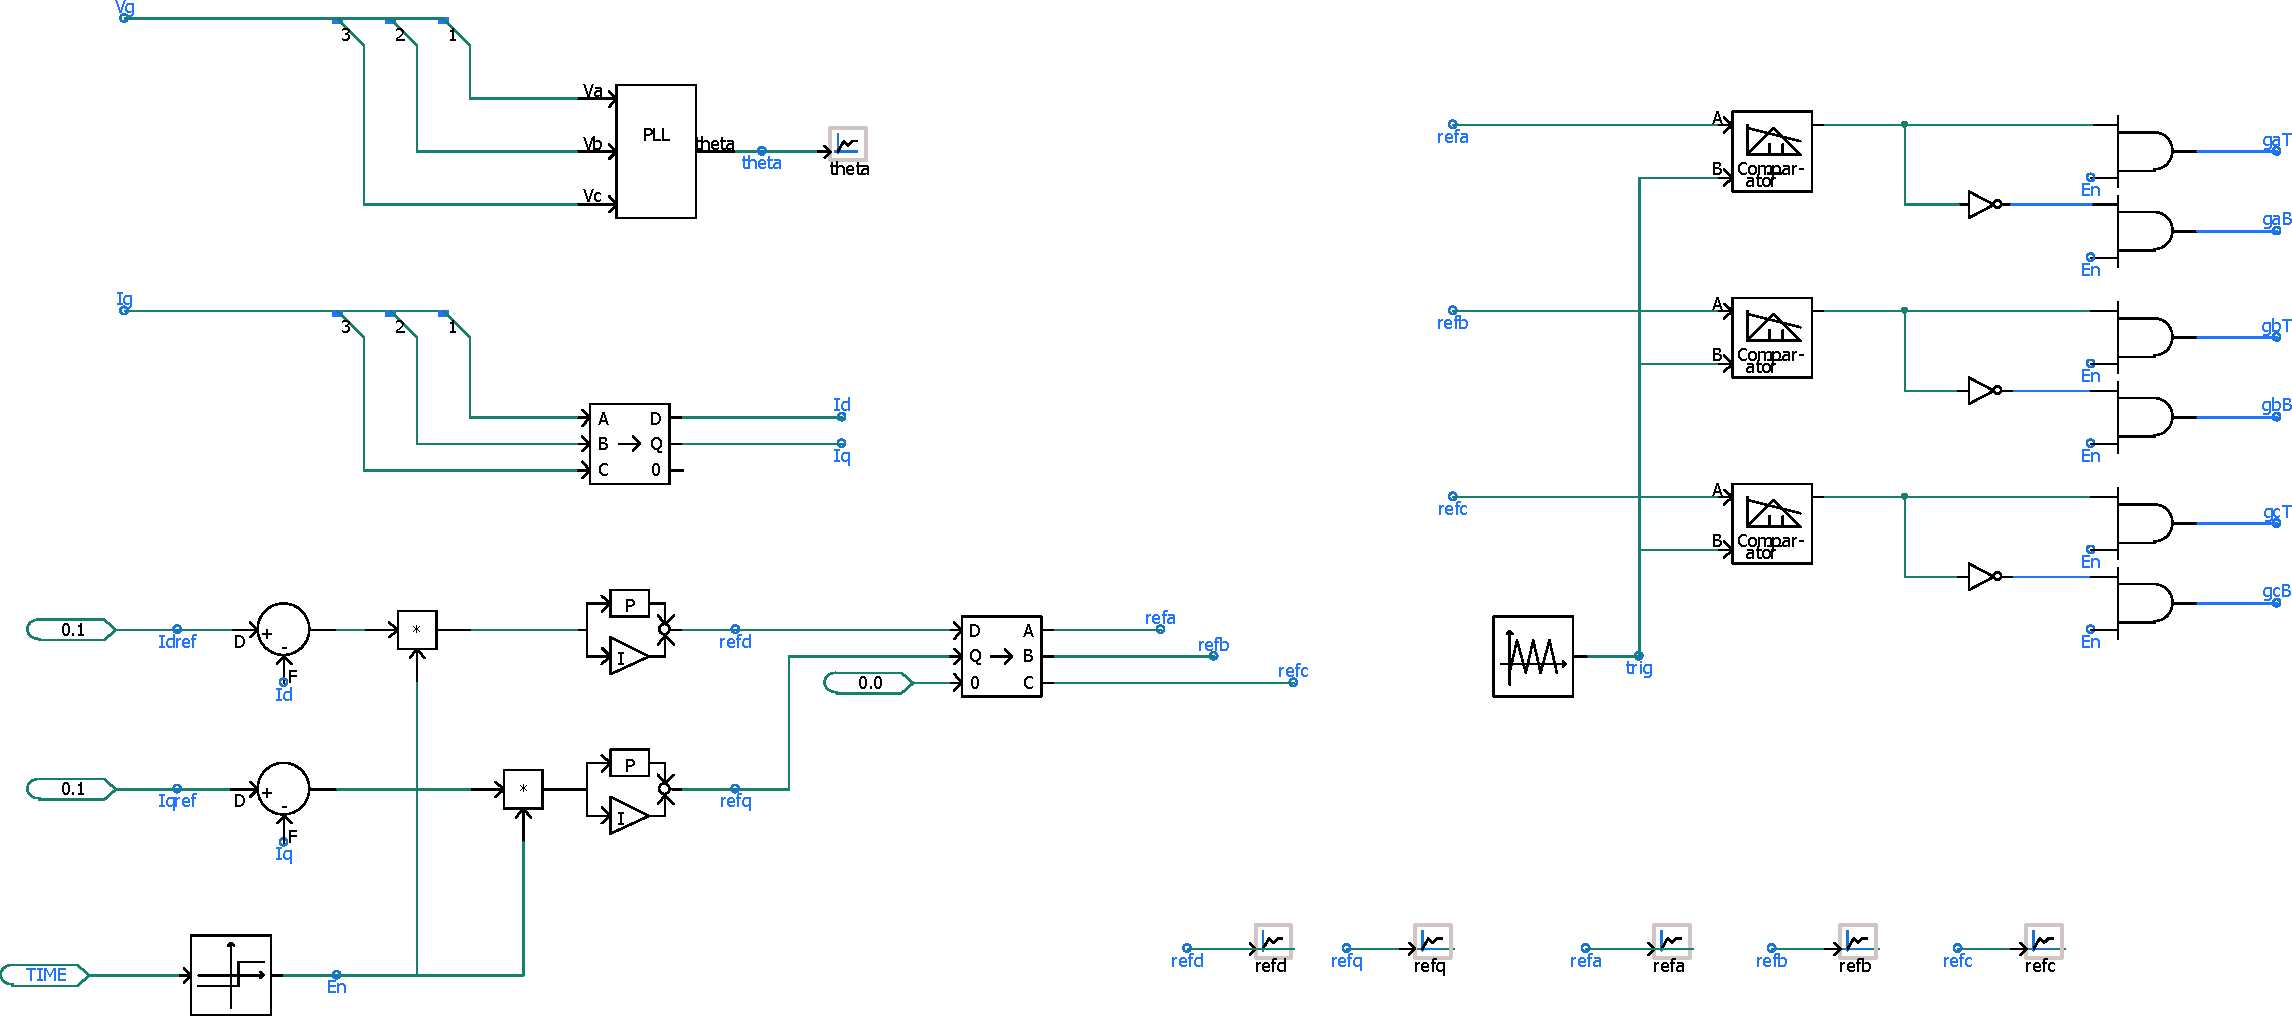
\includegraphics[width=0.75\linewidth]{./figuras/Terceiro-Circuito/SIM6b_CTRL}


\end{frame}




\cmfnewsection{Exportando Dados}{./logos/fundo_tese}{0.15}






%%%%%%%%%%%%%%%%%%%%%%%%%%%%%%%%%%%%%%%%%%%%%%%%
%%%%%%%%%%%%%%%%%%%%%%%%%%%%%%%%%%%%%%%%%%%%%%%%
%%%%%%%%%%%%%%%%%%%%%%%%%%%%%%%%%%%%%%%%%%%%%%%%
%%%%%%%%%%%%%%%%%%%%%%%%%%%%%%%%%%%%%%%%%%%%%%%%
\begin{frame}{Porque Exportar Dados?}
\centering


\textbf{Motivo 1:} Para produzir gráficos com melhor qualidade 
\vspace*{1cm}

\begin{columns}

\column{0.5\linewidth}
\centering
\textbf{PSCAD}
\vspace*{0.5cm}

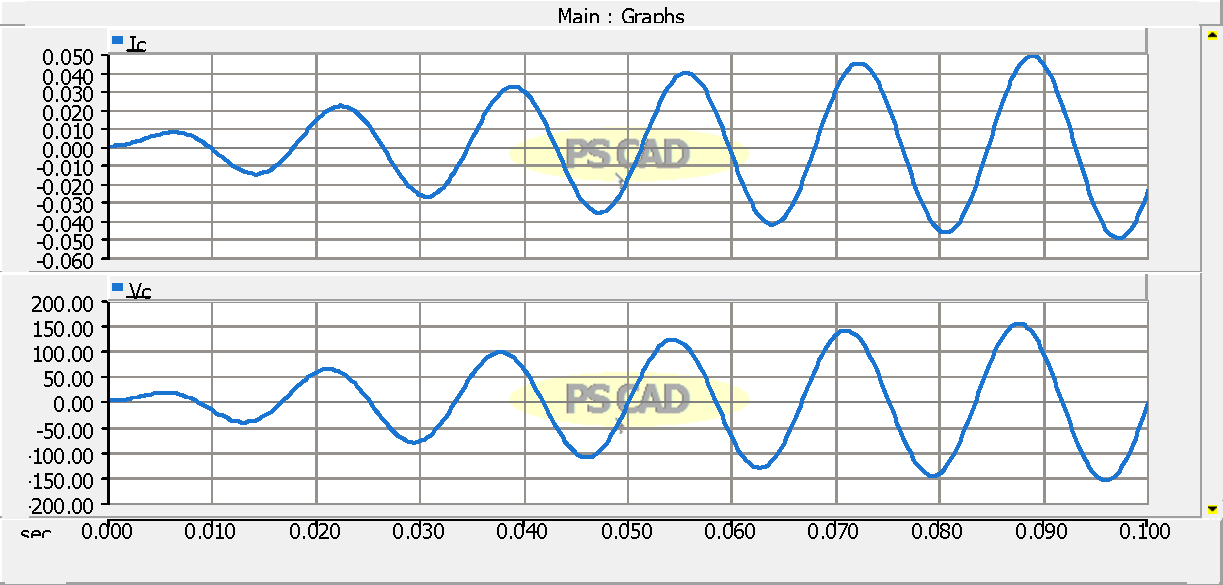
\includegraphics[width=0.90\linewidth]{./figuras/Exportacao/ex_pscadfig}
\column{0.5\linewidth}
\centering
\textbf{MATLAB/OCTAVE/matplotlib/etc}
\vspace*{0.5cm}

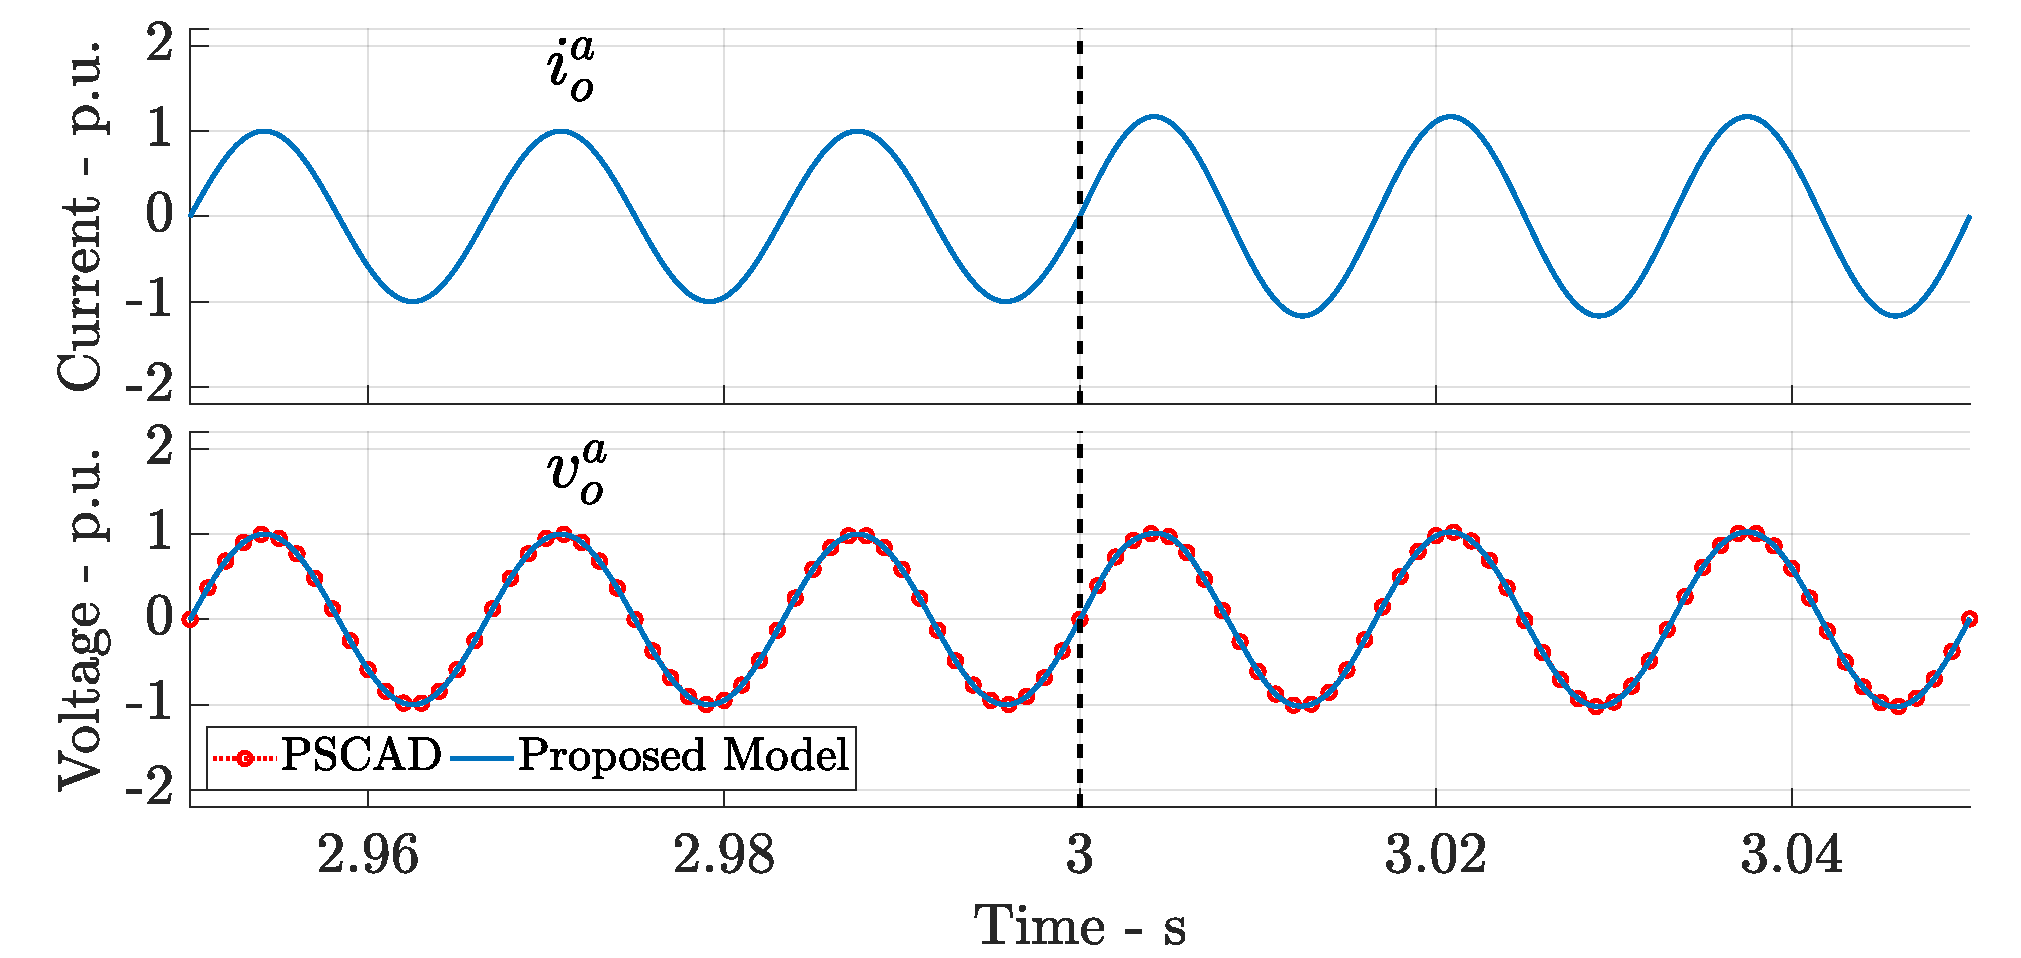
\includegraphics[width=0.90\linewidth]{./figuras/Exportacao/ex_matlab}

\end{columns}

\end{frame}





%%%%%%%%%%%%%%%%%%%%%%%%%%%%%%%%%%%%%%%%%%%%%%%%
%%%%%%%%%%%%%%%%%%%%%%%%%%%%%%%%%%%%%%%%%%%%%%%%
%%%%%%%%%%%%%%%%%%%%%%%%%%%%%%%%%%%%%%%%%%%%%%%%
%%%%%%%%%%%%%%%%%%%%%%%%%%%%%%%%%%%%%%%%%%%%%%%%
\begin{frame}{Porque Exportar Dados?}
\centering


\textbf{Motivo 2:} Para produzir gráficos de variáveis/funções indiretamente obtidas
\vspace*{1cm}

\textbf{Diagrama de bode}
\vspace*{0.5cm}

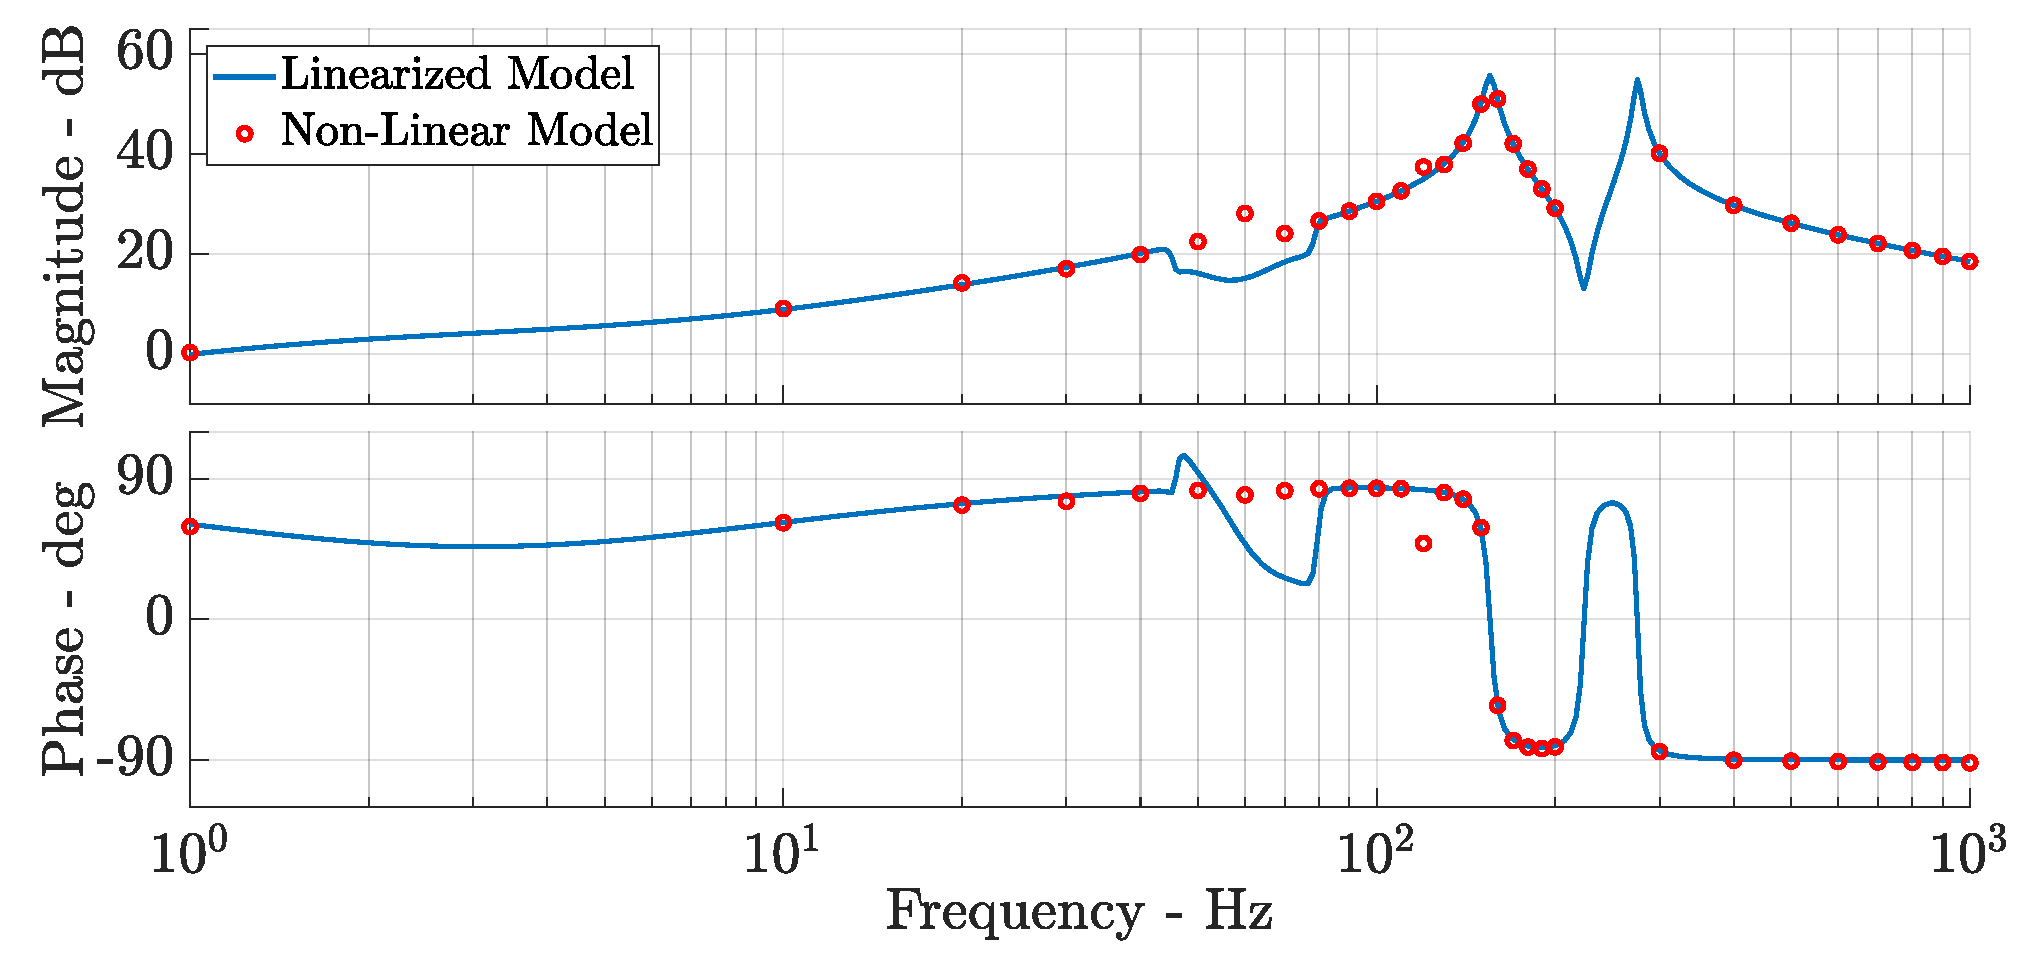
\includegraphics[width=0.60\linewidth]{./figuras/Exportacao/ex_indireto}

\end{frame}






%%%%%%%%%%%%%%%%%%%%%%%%%%%%%%%%%%%%%%%%%%%%%%%%
%%%%%%%%%%%%%%%%%%%%%%%%%%%%%%%%%%%%%%%%%%%%%%%%
%%%%%%%%%%%%%%%%%%%%%%%%%%%%%%%%%%%%%%%%%%%%%%%%
%%%%%%%%%%%%%%%%%%%%%%%%%%%%%%%%%%%%%%%%%%%%%%%%
\begin{frame}{Porque Exportar Dados?}
\centering


\textbf{Motivo 3:} Para Processar Dados
\vspace*{0.5cm}

\textbf{Ex:} Extração de componentes simétricas no domínio do tempo\footnote[frame]{\tiny Verônica Rodrigues Feijão, \href{https://drive.google.com/file/d/1xZGZLela_iNW0KIjTQ59YyCL1-sb16IO/view}{Estudo de Localização de Faltas de Curta Duração para uma Rede de 14 Barras}. Projeto de Graduação -  UERJ, 2019.}
\vspace*{0.5cm}

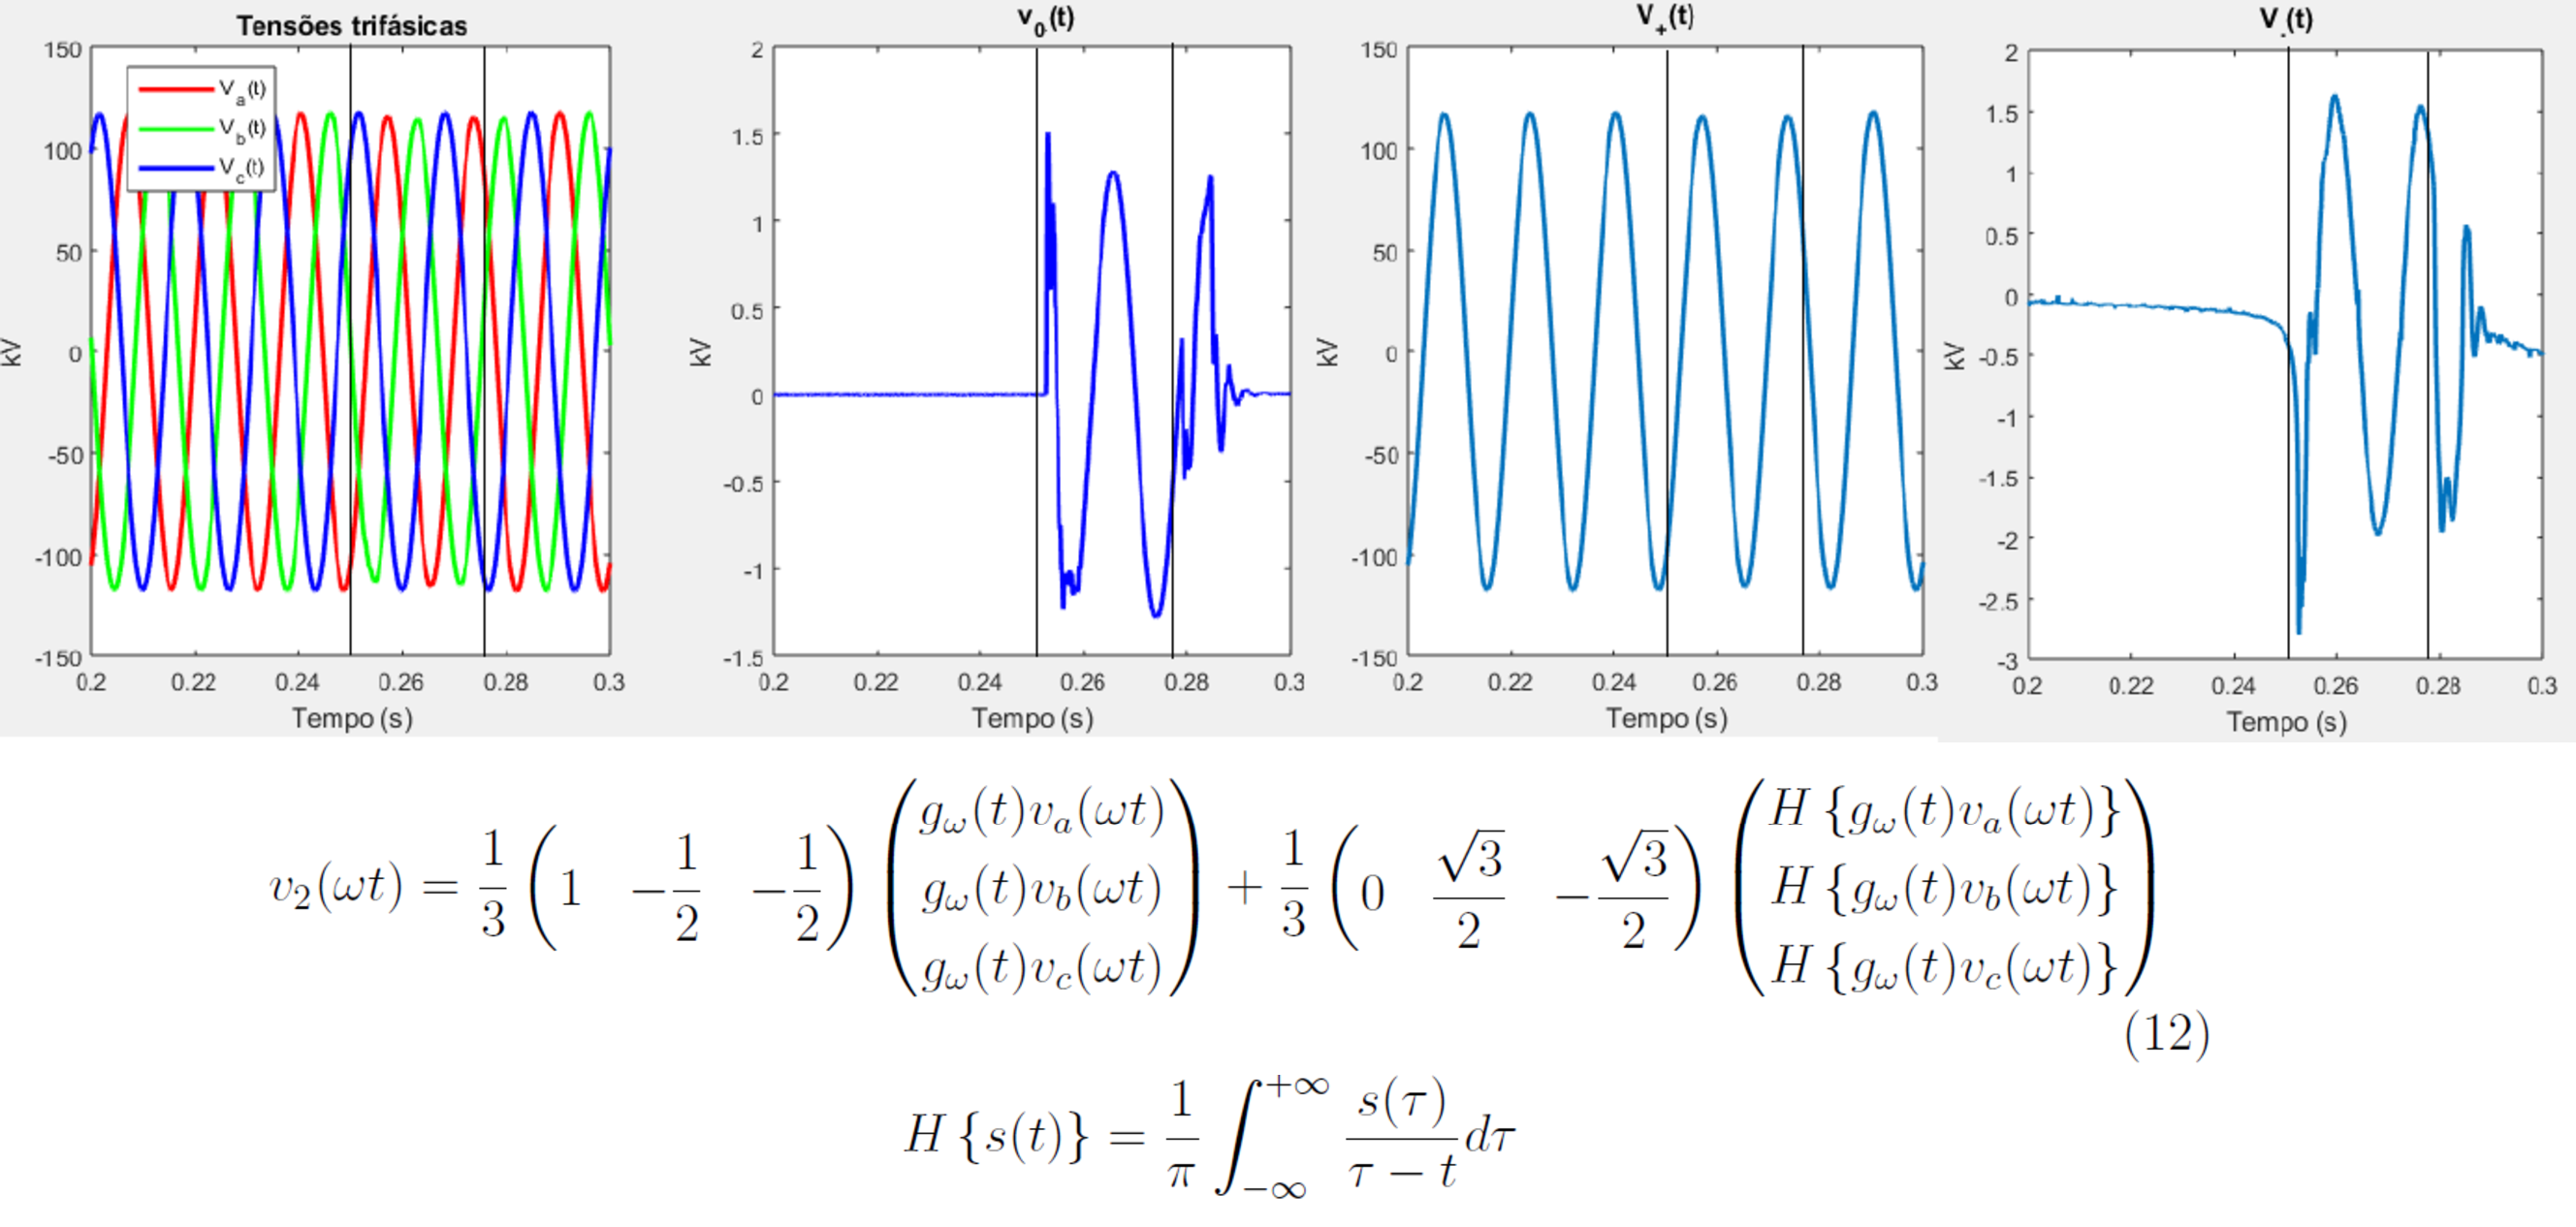
\includegraphics[width=0.65\linewidth]{./figuras/Exportacao/ex_processamento}


\end{frame}






%%%%%%%%%%%%%%%%%%%%%%%%%%%%%%%%%%%%%%%%%%%%%%%%
%%%%%%%%%%%%%%%%%%%%%%%%%%%%%%%%%%%%%%%%%%%%%%%%
%%%%%%%%%%%%%%%%%%%%%%%%%%%%%%%%%%%%%%%%%%%%%%%%
%%%%%%%%%%%%%%%%%%%%%%%%%%%%%%%%%%%%%%%%%%%%%%%%
\begin{frame}{Primeira Possibilidade: Serve para Pequenas Tarefas}
\centering

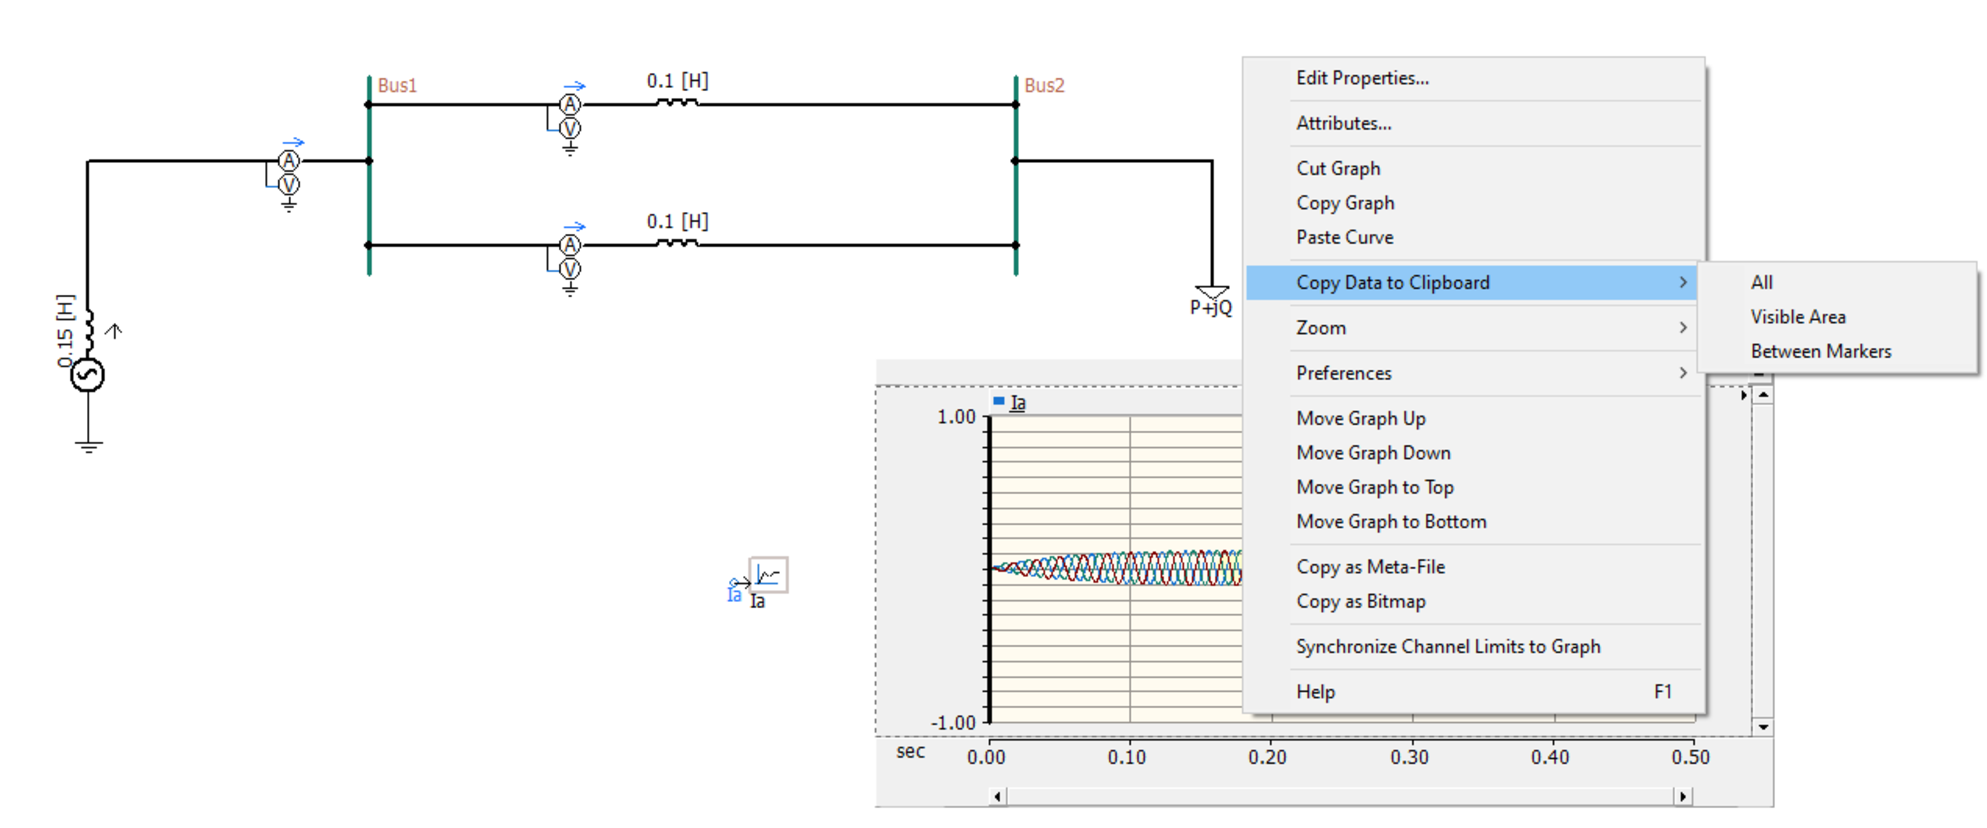
\includegraphics[width=0.95\linewidth]{./figuras/Exportacao/Export1}



\end{frame}




%%%%%%%%%%%%%%%%%%%%%%%%%%%%%%%%%%%%%%%%%%%%%%%%
%%%%%%%%%%%%%%%%%%%%%%%%%%%%%%%%%%%%%%%%%%%%%%%%
%%%%%%%%%%%%%%%%%%%%%%%%%%%%%%%%%%%%%%%%%%%%%%%%
%%%%%%%%%%%%%%%%%%%%%%%%%%%%%%%%%%%%%%%%%%%%%%%%
\begin{frame}{Primeira Possibilidade: Serve para Pequenas Tarefas}
\centering

É só colar em um arquivo de texto:

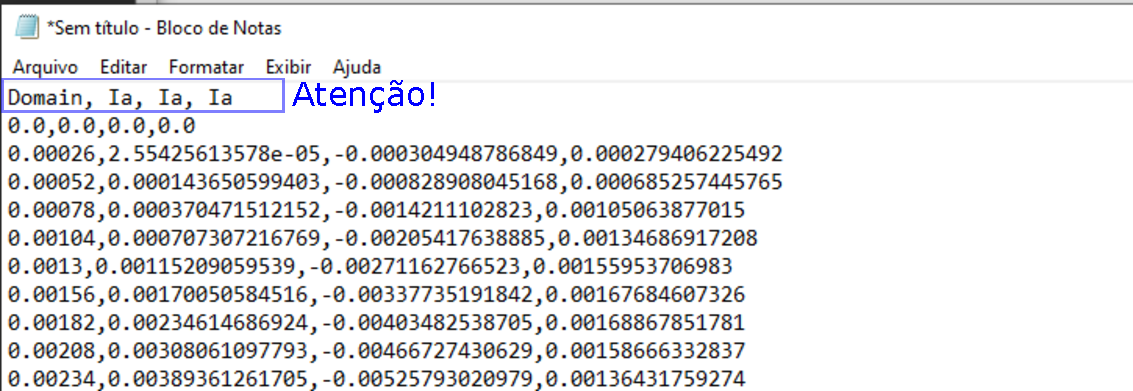
\includegraphics[width=0.95\linewidth]{./figuras/Exportacao/Export1-arquivo}



\end{frame}







%%%%%%%%%%%%%%%%%%%%%%%%%%%%%%%%%%%%%%%%%%%%%%%%
%%%%%%%%%%%%%%%%%%%%%%%%%%%%%%%%%%%%%%%%%%%%%%%%
%%%%%%%%%%%%%%%%%%%%%%%%%%%%%%%%%%%%%%%%%%%%%%%%
%%%%%%%%%%%%%%%%%%%%%%%%%%%%%%%%%%%%%%%%%%%%%%%%
\begin{frame}{Segunda Possibilidade: Útil para Grandes Tarefas}
\centering


\begin{columns}

\column{0.5\linewidth}
\begin{itemize}
\item Podemos configurar a simulação para salvar os dados dos {\i output chanels}
\vspace*{0.5cm}
\item Basta configurar a opção {\it save to disk}
\vspace*{0.5cm}
\item É gerado um arquivo com extensão {\color{blue}\it .map} contendo informações
\vspace*{0.5cm}
\item São gerados aquivos com extensão {\color{blue}\it .out} contendo os dados
\end{itemize}

\column{0.5\linewidth}
\centering
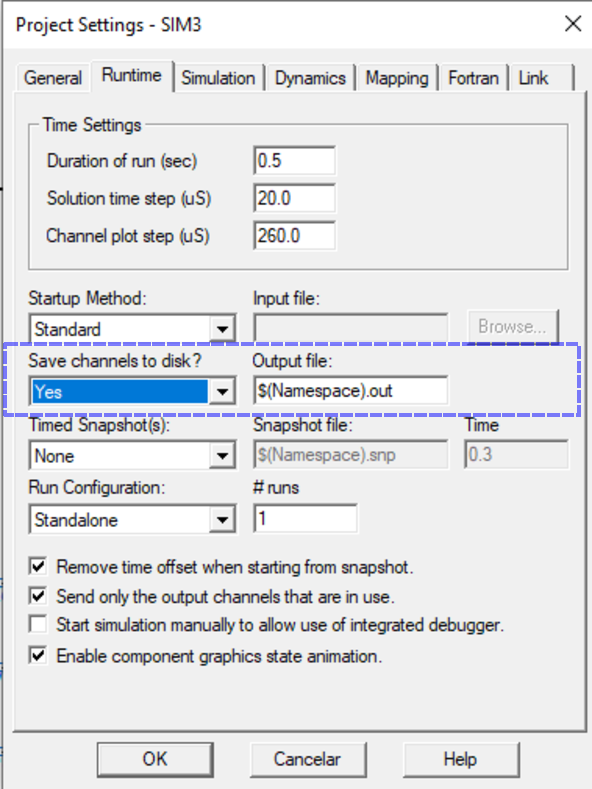
\includegraphics[width=0.70\linewidth]{./figuras/Exportacao/Export2}

\end{columns}


\end{frame}







%%%%%%%%%%%%%%%%%%%%%%%%%%%%%%%%%%%%%%%%%%%%%%%%
%%%%%%%%%%%%%%%%%%%%%%%%%%%%%%%%%%%%%%%%%%%%%%%%
%%%%%%%%%%%%%%%%%%%%%%%%%%%%%%%%%%%%%%%%%%%%%%%%
%%%%%%%%%%%%%%%%%%%%%%%%%%%%%%%%%%%%%%%%%%%%%%%%
\begin{frame}{Segunda Possibilidade: Útil para Grandes Tarefas}
\centering


\begin{columns}

\column{0.5\linewidth}
\begin{itemize}
\item Os arquivos {\color{blue}\it .out} e {\color{blue}\it .map} são dispostos na pasta de arquivos compilados da simulação
\vspace*{1cm}
\item Cada arquivo {\color{blue}\it .out} têm até 10 sinais, um por coluna
\vspace*{1cm}
\item A primeira coluna de todos os arquivos {\color{blue}\it .out} contém o vetor de domínio (Tempo ou Frequência)  
\end{itemize}

\column{0.5\linewidth}
\centering
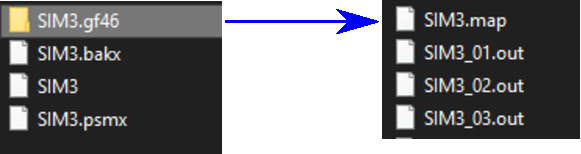
\includegraphics[width=0.70\linewidth]{./figuras/Exportacao/Export2-files}


\end{columns}


\end{frame}






%%%%%%%%%%%%%%%%%%%%%%%%%%%%%%%%%%%%%%%%%%%%%%%%
%%%%%%%%%%%%%%%%%%%%%%%%%%%%%%%%%%%%%%%%%%%%%%%%
%%%%%%%%%%%%%%%%%%%%%%%%%%%%%%%%%%%%%%%%%%%%%%%%
%%%%%%%%%%%%%%%%%%%%%%%%%%%%%%%%%%%%%%%%%%%%%%%%
\begin{frame}{Segunda Possibilidade: Útil para Grandes Tarefas}
\centering


\begin{columns}

\column{0.5\linewidth}
\centering
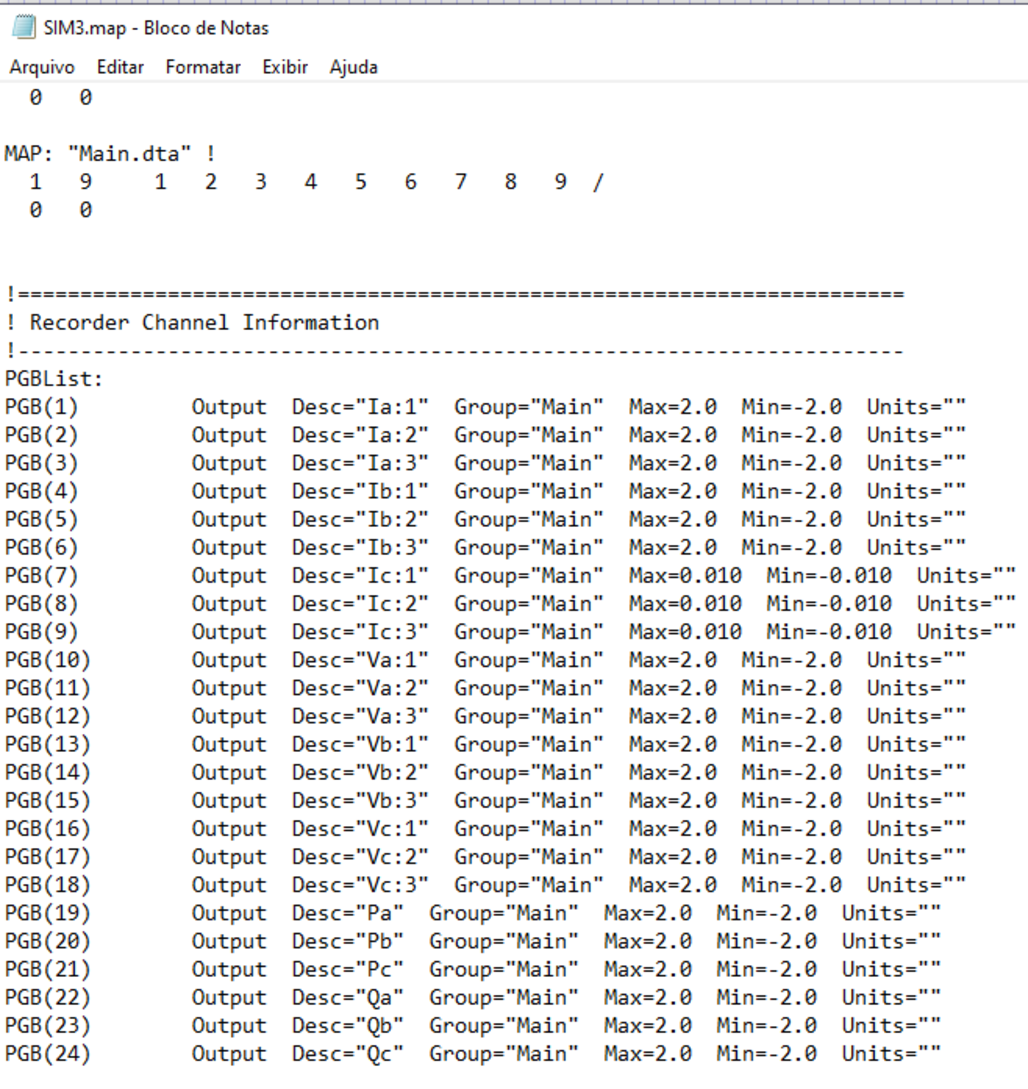
\includegraphics[width=0.80\linewidth]{./figuras/Exportacao/Export2-map}

\column{0.5\linewidth}
\centering
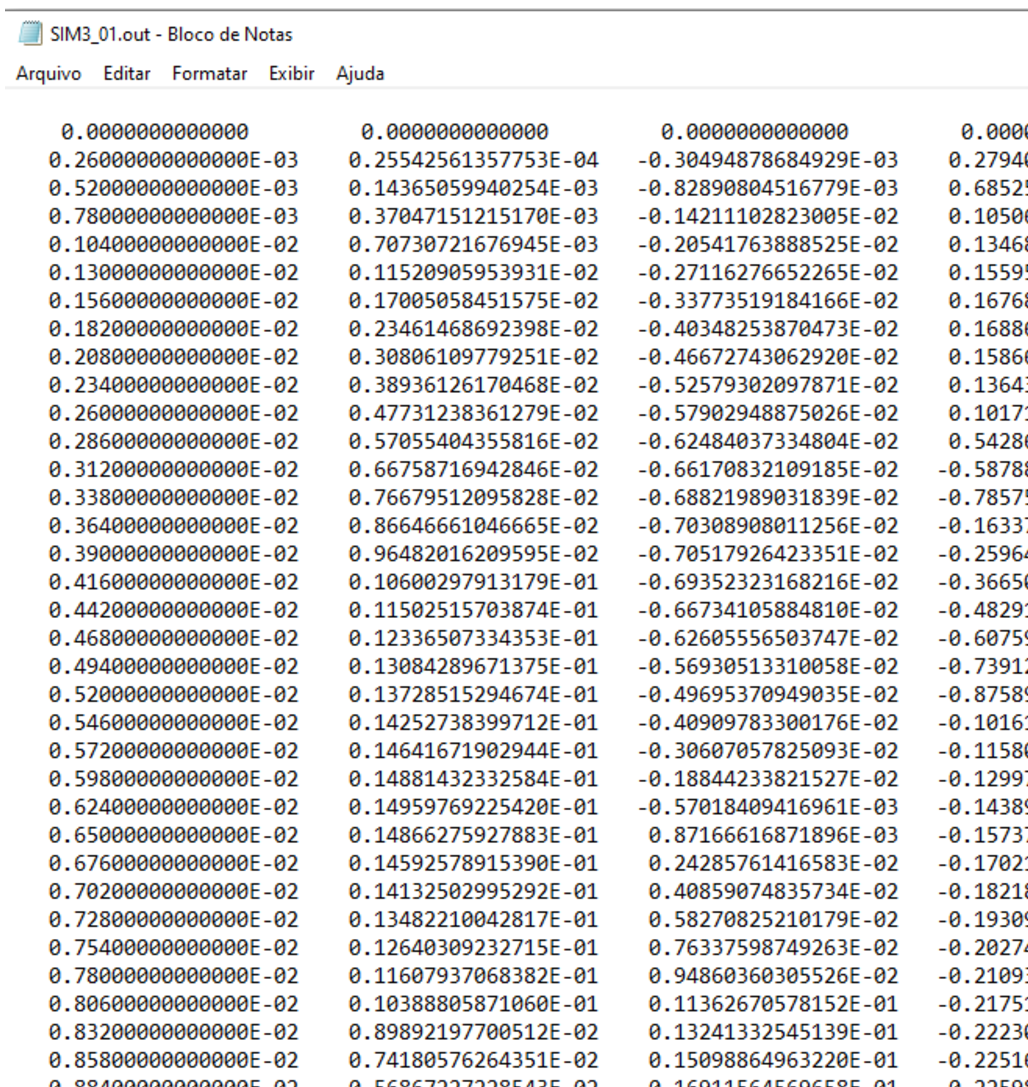
\includegraphics[width=0.80\linewidth]{./figuras/Exportacao/Export2-out}


\end{columns}


\end{frame}



\cmfnewsection{Automação de Simulações}{./logos/fundo_tese}{0.15}





%%%%%%%%%%%%%%%%%%%%%%%%%%%%%%%%%%%%%%%%%%%%%%%%
%%%%%%%%%%%%%%%%%%%%%%%%%%%%%%%%%%%%%%%%%%%%%%%%
%%%%%%%%%%%%%%%%%%%%%%%%%%%%%%%%%%%%%%%%%%%%%%%%
%%%%%%%%%%%%%%%%%%%%%%%%%%%%%%%%%%%%%%%%%%%%%%%%
\begin{frame}{O que significa automatizar simulações?}
\centering


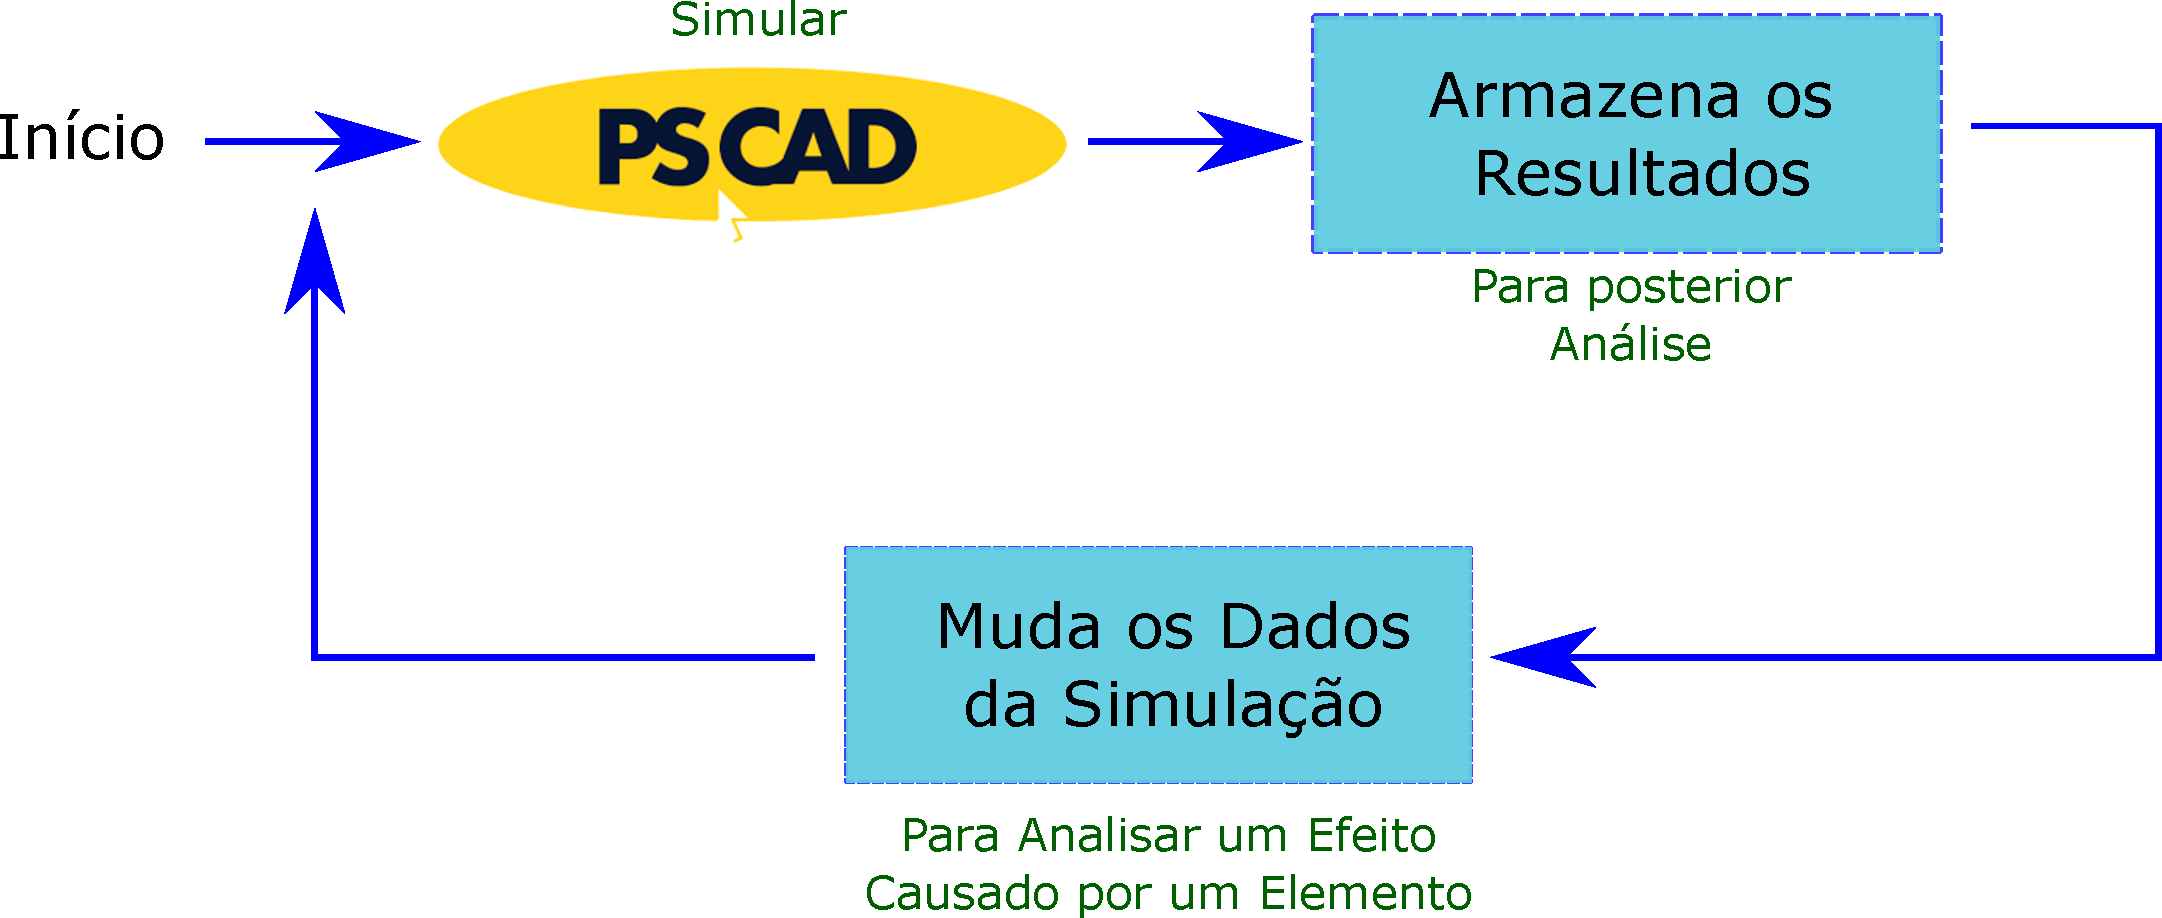
\includegraphics[width=0.80\linewidth]{./figuras/Automacao/automa}


\end{frame}





%%%%%%%%%%%%%%%%%%%%%%%%%%%%%%%%%%%%%%%%%%%%%%%%
%%%%%%%%%%%%%%%%%%%%%%%%%%%%%%%%%%%%%%%%%%%%%%%%
%%%%%%%%%%%%%%%%%%%%%%%%%%%%%%%%%%%%%%%%%%%%%%%%
%%%%%%%%%%%%%%%%%%%%%%%%%%%%%%%%%%%%%%%%%%%%%%%%
\begin{frame}{Por que automatizar simulações?}
\centering

\textbf{Motivo 1:} Ajustar sistemas de controle
\vspace*{0.5cm}

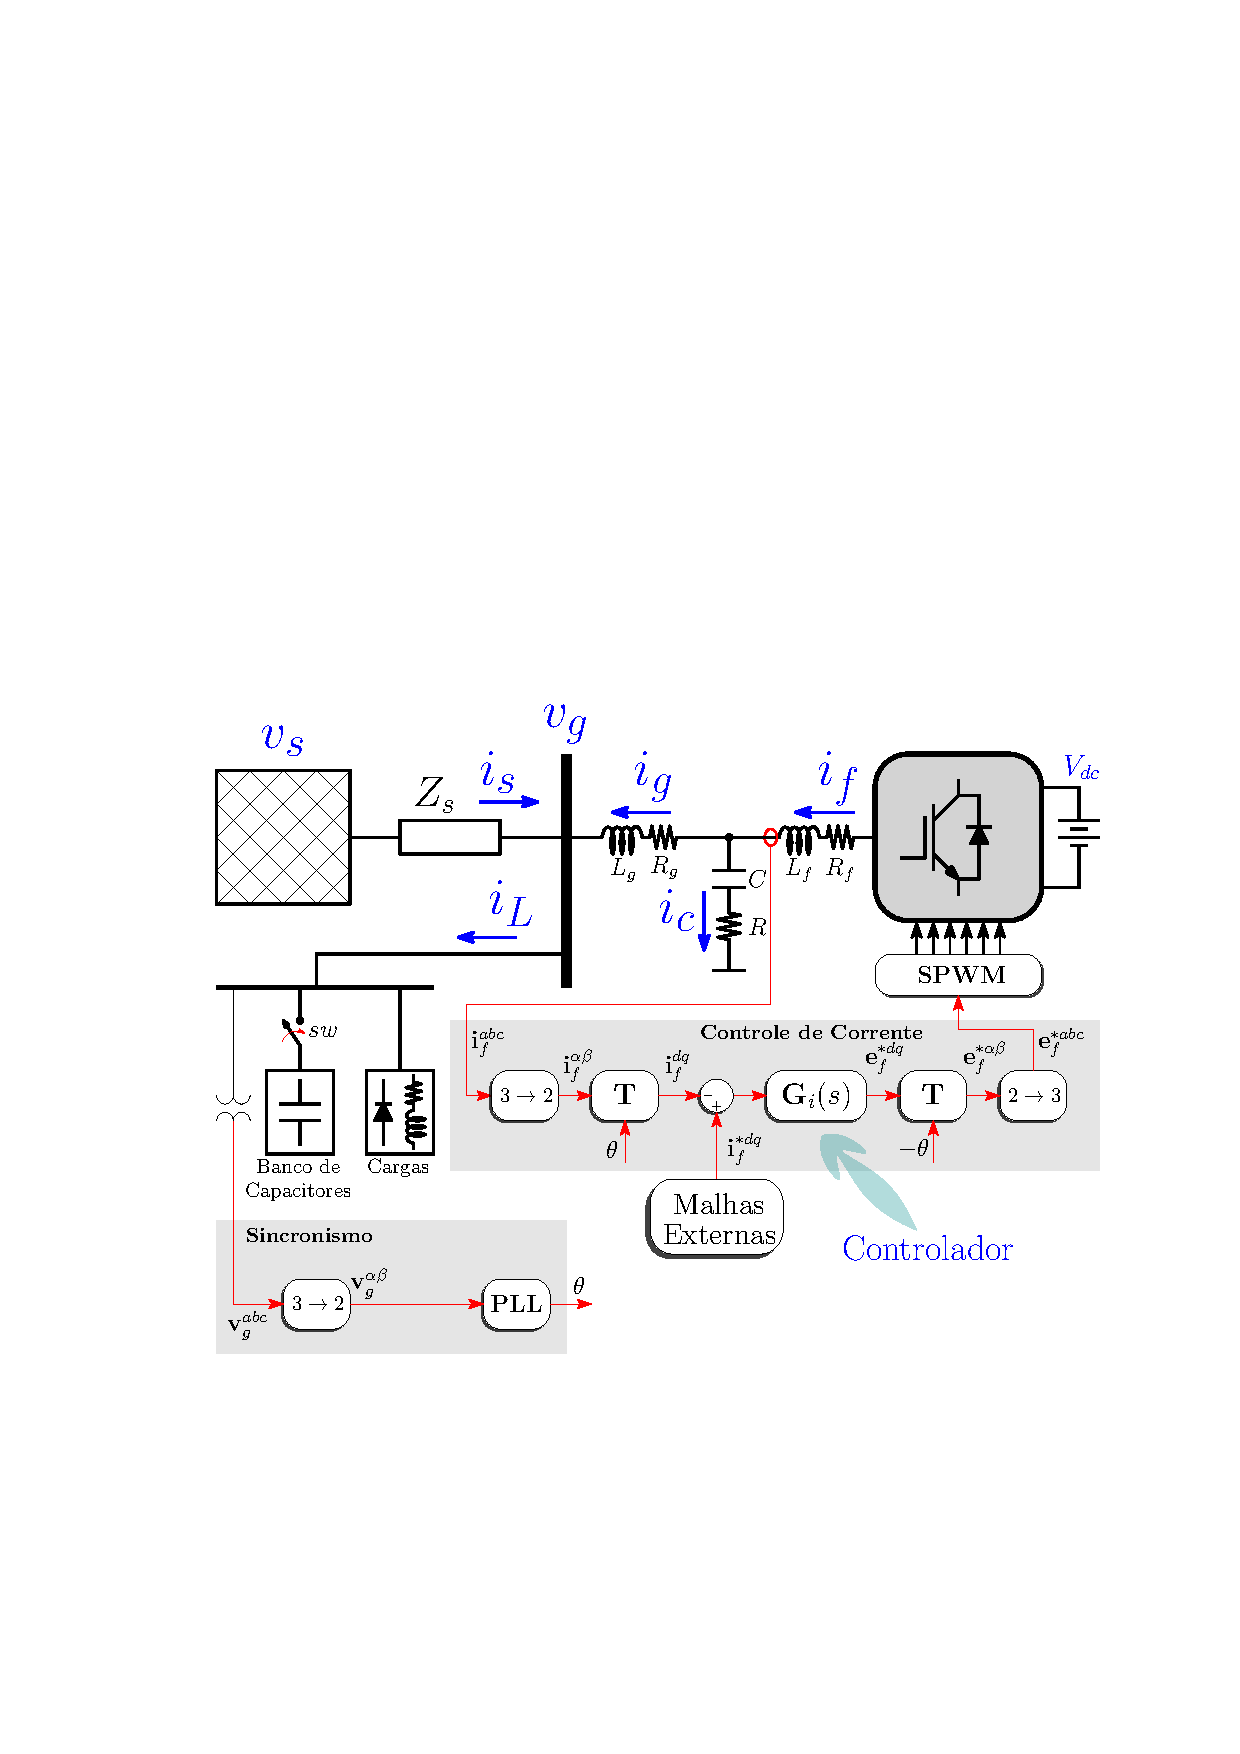
\includegraphics[width=0.55\linewidth]{./figuras/Automacao/SISTEMA}

\end{frame}







%%%%%%%%%%%%%%%%%%%%%%%%%%%%%%%%%%%%%%%%%%%%%%%%
%%%%%%%%%%%%%%%%%%%%%%%%%%%%%%%%%%%%%%%%%%%%%%%%
%%%%%%%%%%%%%%%%%%%%%%%%%%%%%%%%%%%%%%%%%%%%%%%%
%%%%%%%%%%%%%%%%%%%%%%%%%%%%%%%%%%%%%%%%%%%%%%%%
\begin{frame}{Por que automatizar simulações?}
\centering

\textbf{Motivo 2:} Avaliar efeitos de eventos em diferentes pontos em um sistema grande\footnote[frame]{\tiny Verônica Rodrigues Feijão, \href{https://drive.google.com/file/d/1xZGZLela_iNW0KIjTQ59YyCL1-sb16IO/view}{Estudo de Localização de Faltas de Curta Duração para uma Rede de 14 Barras}. Projeto de Graduação -  UERJ, 2019.}
%\vspace*{1cm}

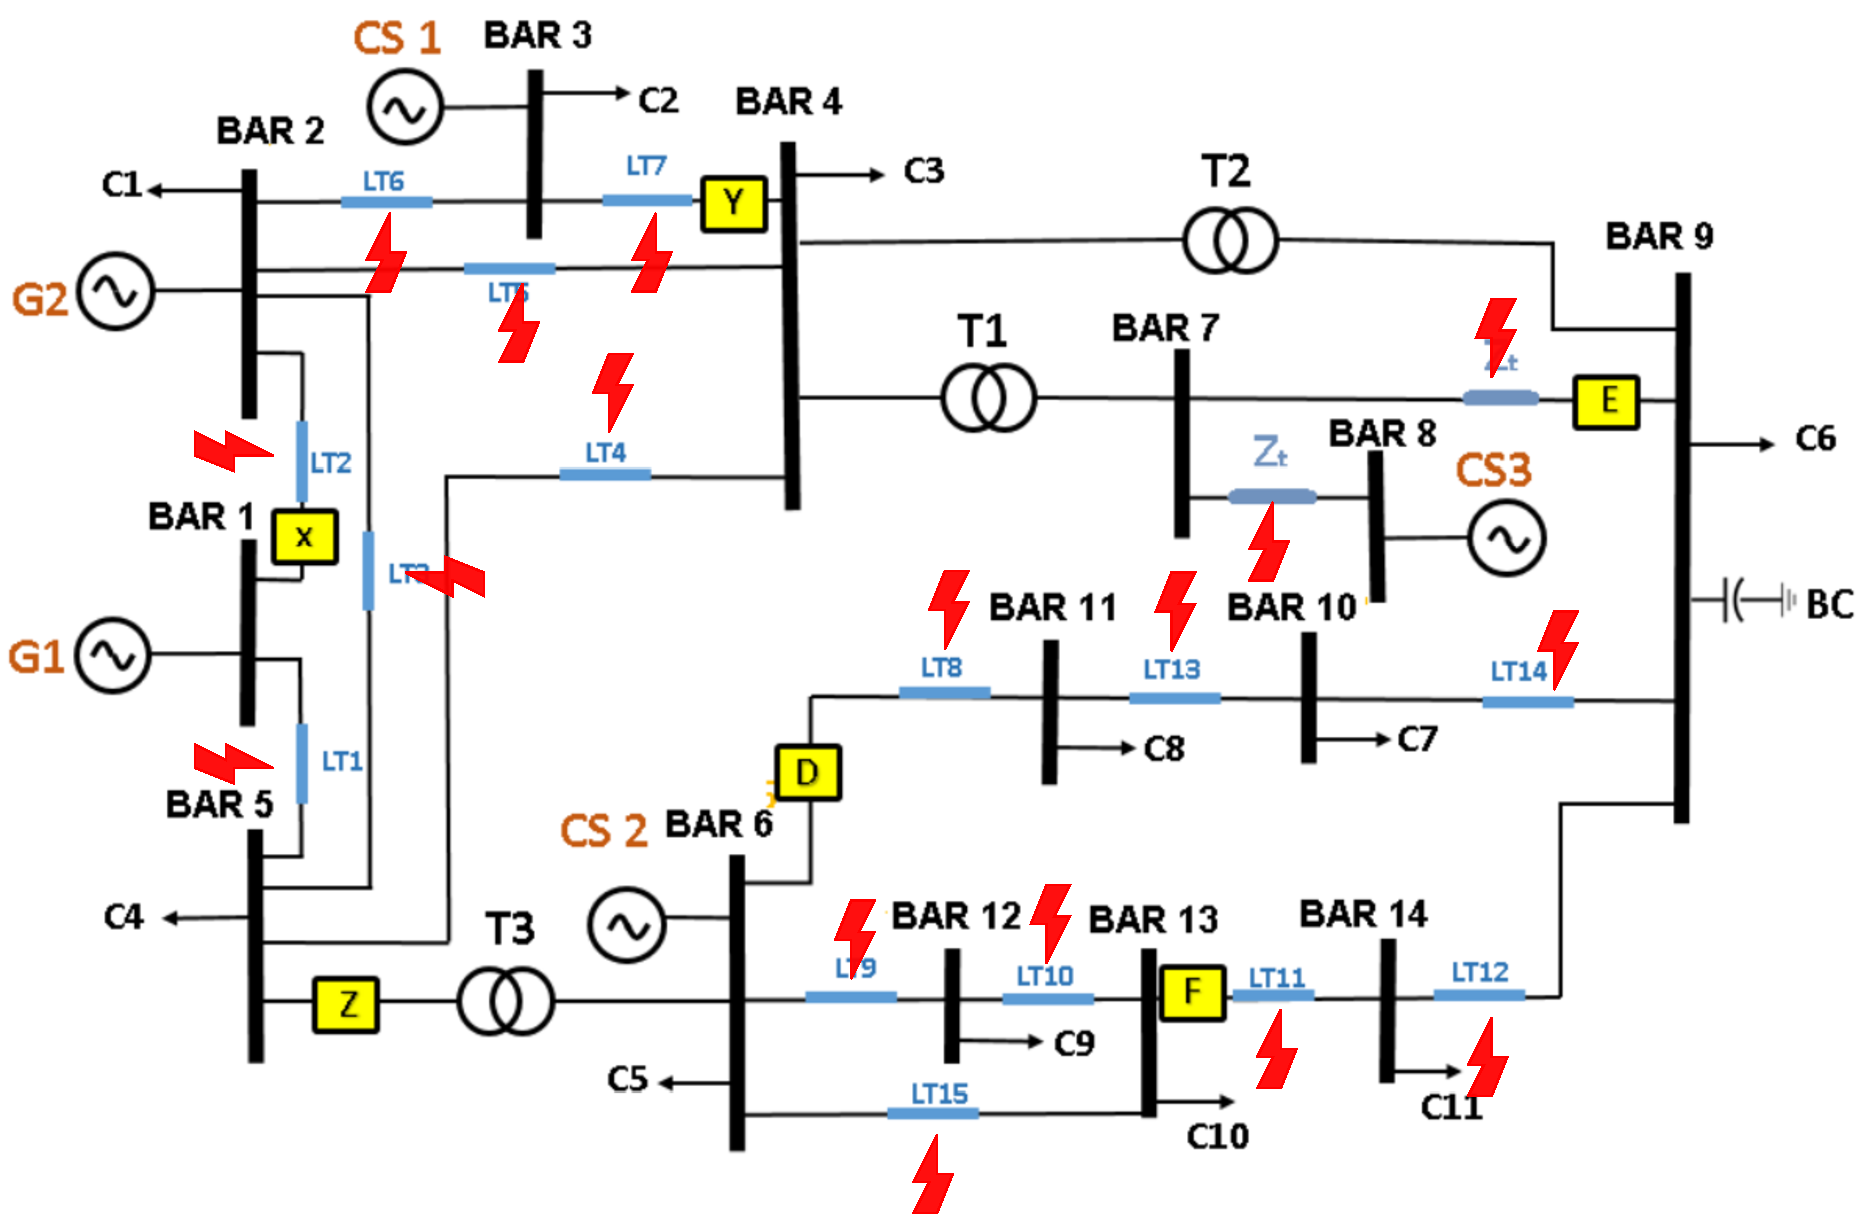
\includegraphics[width=0.6\linewidth]{./figuras/Automacao/ex_curto}

\end{frame}





%%%%%%%%%%%%%%%%%%%%%%%%%%%%%%%%%%%%%%%%%%%%%%%%
%%%%%%%%%%%%%%%%%%%%%%%%%%%%%%%%%%%%%%%%%%%%%%%%
%%%%%%%%%%%%%%%%%%%%%%%%%%%%%%%%%%%%%%%%%%%%%%%%
%%%%%%%%%%%%%%%%%%%%%%%%%%%%%%%%%%%%%%%%%%%%%%%%
\begin{frame}{Como fazer?}
\centering

\begin{columns}


\column{0.5\linewidth}

\begin{itemize}
\item Inserir/Configurar o bloco {\it Multiple run} localizado no grupo de {\it I/O Devices} na biblioteca Master.

\vspace*{2.5cm}

\item Configurar o projeto para {\it Multiple run}.

\vspace*{1cm}
\end{itemize}


\column{0.5\linewidth}
\includegraphics[width=0.80\linewidth]{./figuras/Automacao/multrun}

\end{columns}

\end{frame}




%%%%%%%%%%%%%%%%%%%%%%%%%%%%%%%%%%%%%%%%%%%%%%%%
%%%%%%%%%%%%%%%%%%%%%%%%%%%%%%%%%%%%%%%%%%%%%%%%
%%%%%%%%%%%%%%%%%%%%%%%%%%%%%%%%%%%%%%%%%%%%%%%%
%%%%%%%%%%%%%%%%%%%%%%%%%%%%%%%%%%%%%%%%%%%%%%%%
\begin{frame}{Circuito Exemplo}
\centering

\includegraphics[width=0.85\linewidth]{./figuras/Automacao/SIM}

\end{frame}
\cmfnewsection{Criação de Componentes e Bibliotecas}{./logos/fundo_tese}{0.15}







%%%%%%%%%%%%%%%%%%%%%%%%%%%%%%%%%%%%%%%%%%%%%%%%
%%%%%%%%%%%%%%%%%%%%%%%%%%%%%%%%%%%%%%%%%%%%%%%%
%%%%%%%%%%%%%%%%%%%%%%%%%%%%%%%%%%%%%%%%%%%%%%%%
%%%%%%%%%%%%%%%%%%%%%%%%%%%%%%%%%%%%%%%%%%%%%%%%
\begin{frame}{Encapsulando Circuitos: {\it Component Wizard}}
\centering


\includegraphics[width=0.75\linewidth]{./figuras/Componentes/wizard}


\end{frame}





%%%%%%%%%%%%%%%%%%%%%%%%%%%%%%%%%%%%%%%%%%%%%%%%
%%%%%%%%%%%%%%%%%%%%%%%%%%%%%%%%%%%%%%%%%%%%%%%%
%%%%%%%%%%%%%%%%%%%%%%%%%%%%%%%%%%%%%%%%%%%%%%%%
%%%%%%%%%%%%%%%%%%%%%%%%%%%%%%%%%%%%%%%%%%%%%%%%
\begin{frame}{Encapsulando Circuitos: Resultado}
\centering


\includegraphics[width=0.45\linewidth]{./figuras/Componentes/componenteTeste}


\end{frame}




%%%%%%%%%%%%%%%%%%%%%%%%%%%%%%%%%%%%%%%%%%%%%%%%
%%%%%%%%%%%%%%%%%%%%%%%%%%%%%%%%%%%%%%%%%%%%%%%%
%%%%%%%%%%%%%%%%%%%%%%%%%%%%%%%%%%%%%%%%%%%%%%%%
%%%%%%%%%%%%%%%%%%%%%%%%%%%%%%%%%%%%%%%%%%%%%%%%
\begin{frame}{Encapsulando Circuitos: Montando o Esquemático}
\centering


\includegraphics[width=0.75\linewidth]{./figuras/Componentes/schematico}


\end{frame}







%%%%%%%%%%%%%%%%%%%%%%%%%%%%%%%%%%%%%%%%%%%%%%%%
%%%%%%%%%%%%%%%%%%%%%%%%%%%%%%%%%%%%%%%%%%%%%%%%
%%%%%%%%%%%%%%%%%%%%%%%%%%%%%%%%%%%%%%%%%%%%%%%%
%%%%%%%%%%%%%%%%%%%%%%%%%%%%%%%%%%%%%%%%%%%%%%%%
\begin{frame}{Encapsulando Circuitos: Testando}
\centering


\includegraphics[width=0.75\linewidth]{./figuras/Componentes/Testando}


\end{frame}






%%%%%%%%%%%%%%%%%%%%%%%%%%%%%%%%%%%%%%%%%%%%%%%%
%%%%%%%%%%%%%%%%%%%%%%%%%%%%%%%%%%%%%%%%%%%%%%%%
%%%%%%%%%%%%%%%%%%%%%%%%%%%%%%%%%%%%%%%%%%%%%%%%
%%%%%%%%%%%%%%%%%%%%%%%%%%%%%%%%%%%%%%%%%%%%%%%%
\begin{frame}{Encapsulando Circuitos: {\it Decorando o Bloco}}
\centering


\includegraphics[width=0.75\linewidth]{./figuras/Componentes/grafica}


\end{frame}






%%%%%%%%%%%%%%%%%%%%%%%%%%%%%%%%%%%%%%%%%%%%%%%%
%%%%%%%%%%%%%%%%%%%%%%%%%%%%%%%%%%%%%%%%%%%%%%%%
%%%%%%%%%%%%%%%%%%%%%%%%%%%%%%%%%%%%%%%%%%%%%%%%
%%%%%%%%%%%%%%%%%%%%%%%%%%%%%%%%%%%%%%%%%%%%%%%%
\begin{frame}{Encapsulando Circuitos: Testando, de novo}
\centering


\includegraphics[width=0.75\linewidth]{./figuras/Componentes/Testando2}


\end{frame}




%%%%%%%%%%%%%%%%%%%%%%%%%%%%%%%%%%%%%%%%%%%%%%%%
%%%%%%%%%%%%%%%%%%%%%%%%%%%%%%%%%%%%%%%%%%%%%%%%
%%%%%%%%%%%%%%%%%%%%%%%%%%%%%%%%%%%%%%%%%%%%%%%%
%%%%%%%%%%%%%%%%%%%%%%%%%%%%%%%%%%%%%%%%%%%%%%%%
\begin{frame}{Programando componentes com FORTRAN}
\centering

\begin{columns}


\column{0.5\linewidth}
\begin{itemize}
\item Criar um bloco seguindo os passos anteriores
\vspace*{1cm}
\item Demarcar a opção {\it Module}
\vspace*{1cm}
\item Programar o bloco na aba script
\end{itemize}

\column{0.5\linewidth}
\includegraphics[width=0.75\linewidth]{./figuras/Componentes/componenteFortran}

\end{columns}




\end{frame}




%%%%%%%%%%%%%%%%%%%%%%%%%%%%%%%%%%%%%%%%%%%%%%%%
%%%%%%%%%%%%%%%%%%%%%%%%%%%%%%%%%%%%%%%%%%%%%%%%
%%%%%%%%%%%%%%%%%%%%%%%%%%%%%%%%%%%%%%%%%%%%%%%%
%%%%%%%%%%%%%%%%%%%%%%%%%%%%%%%%%%%%%%%%%%%%%%%%
\begin{frame}{Programando componentes com FORTRAN: Componente A}
\centering

Componente que soma uma constante $K$ a todos os elementos de um vetor. Ou seja:
\vspace*{0.5cm}

\begin{equation*}
\mathbf{y}[n] = \mathbf{x}[n] + K 
\end{equation*}
\vspace*{0.5cm}

$\mathbf{y}$ - Vetor com $N$ posições (saída do bloco)
\vspace*{0.5cm}

$\mathbf{x}$ - Vetor com $N$ posições (entrada do bloco)
\vspace*{0.5cm}

$K$ - Constante


\end{frame}





%%%%%%%%%%%%%%%%%%%%%%%%%%%%%%%%%%%%%%%%%%%%%%%%
%%%%%%%%%%%%%%%%%%%%%%%%%%%%%%%%%%%%%%%%%%%%%%%%
%%%%%%%%%%%%%%%%%%%%%%%%%%%%%%%%%%%%%%%%%%%%%%%%
%%%%%%%%%%%%%%%%%%%%%%%%%%%%%%%%%%%%%%%%%%%%%%%%
\begin{frame}{Programando componentes com FORTRAN: Componente A}
\centering

\includegraphics[width=0.75\linewidth]{./figuras/Componentes/FortranA_parameter}

\end{frame}




%%%%%%%%%%%%%%%%%%%%%%%%%%%%%%%%%%%%%%%%%%%%%%%%
%%%%%%%%%%%%%%%%%%%%%%%%%%%%%%%%%%%%%%%%%%%%%%%%
%%%%%%%%%%%%%%%%%%%%%%%%%%%%%%%%%%%%%%%%%%%%%%%%
%%%%%%%%%%%%%%%%%%%%%%%%%%%%%%%%%%%%%%%%%%%%%%%%
\begin{frame}{Programando componentes com FORTRAN: Componente A}
\centering

\includegraphics[width=0.75\linewidth]{./figuras/Componentes/FortranA_script}

\end{frame}




%%%%%%%%%%%%%%%%%%%%%%%%%%%%%%%%%%%%%%%%%%%%%%%%
%%%%%%%%%%%%%%%%%%%%%%%%%%%%%%%%%%%%%%%%%%%%%%%%
%%%%%%%%%%%%%%%%%%%%%%%%%%%%%%%%%%%%%%%%%%%%%%%%
%%%%%%%%%%%%%%%%%%%%%%%%%%%%%%%%%%%%%%%%%%%%%%%%
\begin{frame}{Programando componentes com FORTRAN: Componente B}
\centering

\includegraphics[width=0.45\linewidth]{./figuras/Componentes/FortranB_script}

\end{frame}





%%%%%%%%%%%%%%%%%%%%%%%%%%%%%%%%%%%%%%%%%%%%%%%%
%%%%%%%%%%%%%%%%%%%%%%%%%%%%%%%%%%%%%%%%%%%%%%%%
%%%%%%%%%%%%%%%%%%%%%%%%%%%%%%%%%%%%%%%%%%%%%%%%
%%%%%%%%%%%%%%%%%%%%%%%%%%%%%%%%%%%%%%%%%%%%%%%%
\begin{frame}{Guardando componentes em uma Biblioteca}
\centering

\begin{columns}


\column{0.5\linewidth}

\begin{itemize}
\item Crie uma biblioteca
\vspace*{1cm}
\item No workspace, Copie a definição do componente do seu projeto
\vspace*{1cm}
\item Cole na seção de definições da biblioteca
\end{itemize}
\vspace*{1cm}

\column{0.5\linewidth}
\centering
\vspace*{1cm}

\includegraphics[width=0.75\linewidth]{./figuras/Componentes/lib}


\end{columns}

\end{frame}






%
%\begin{frame}{teste 2}
%teste
%\end{frame}
%
%\include{./Partes/Introducao/Introducao}
%\include{./Partes/Geracao_Solar/Geracao_Solar}





\end{document}